% !TEX root = main.tex
% \documentclass{tufte-book}%[a4paper,twoside]
% See https://github.com/Tufte-LaTeX/tufte-latex/blob/master/sample-book.tex for details

% --- AMAZON BEGIN ---
% WITHOUT BLEED
% US Trade => 6x9
\documentclass[paper=6in:9in,pagesize=pdftex,
               headinclude=on,footinclude=on,12pt]{scrbook}
%
% Paper width
% W = 6in
% Paper height
% H = 9in
% Paper gutter
% BCOR = 0.5in
% Margin (0.5in imposed on lulu, recommended on createspace)
% m = 0.5in
% Text height
% h = H - 2m = 8in
% Text width
% w = W - 2m - BCOR = 4.5in
\areaset[0.50in]{4.5in}{8in}
% --- AMAZON END ---

% Copyright with title BEGIN
\usepackage{fancyhdr}
\def\secondpage{\clearpage\null\vfill
\pagestyle{empty}
\begin{minipage}[b]{0.9\textwidth}
\normalsize 21 Lessons \newline
\footnotesize What I've Learned From Falling Down the Bitcoin Rabbit Hole \par

First edition. Version 0.3.0, git commit \texttt{2e5c5c6}.

\footnotesize\raggedright
\setlength{\parskip}{0.5\baselineskip}
Copyright \copyright 2018--\the\year\ Gigi \par


\includegraphics[width=2cm]{assets/images/cc-by-sa.pdf}

This book and its on-line version are distributed under the terms of the
Creative Commons Attribution-ShareAlike 4.0 license. A reference copy of this
license may be found at the official creative commons
page.\footnote{\url{https://creativecommons.org/licenses/by-sa/4.0}}

\end{minipage}
\vspace*{2\baselineskip}
\cleardoublepage
\rfoot{\thepage}}

\makeatletter
\g@addto@macro{\maketitle}{\secondpage}
\makeatother
% Copyright with title END



% Packages
\usepackage{booktabs}
\usepackage{graphicx}
\setkeys{Gin}{width=\linewidth,totalheight=\textheight,keepaspectratio}
\graphicspath{{graphics/}}

%%
% For Quotes
\usepackage{csquotes}
\renewcommand\mkbegdispquote[2]{\makebox[0pt][r]{\textquotedblleft\,}}
\renewcommand\mkenddispquote[2]{\,\textquotedblright#2}

%%
% Just some sample text
\usepackage{lipsum}

%%
% For nicely typeset tabular material
\usepackage{booktabs}

%%
% Bibliography stuff: Biber, BibTex, BibLatex
%\usepackage[autostyle]{csquotes}
% \usepackage[
    % backend=biber,
    % style=authoryear-icomp,
    % sortlocale=de_DE,
    % natbib=true,
    % url=false,
    % doi=true,
    % eprint=false
% ]{biblatex}
% \usepackage[backend=biber]{biblatex}
\usepackage{url}
\usepackage{natbib}
\bibliographystyle{plain}

%%
% Hyperlinks
\usepackage[hidelinks]{hyperref}

%%
% For graphics / images
\usepackage{graphicx}
\setkeys{Gin}{width=\linewidth,totalheight=\textheight,keepaspectratio}
\graphicspath{{graphics/}}

% The fancyvrb package lets us customize the formatting of verbatim
% environments.  We use a slightly smaller font.
\usepackage{fancyvrb}
\fvset{fontsize=\normalsize}

%%
% Prints argument within hanging parentheses (i.e., parentheses that take
% up no horizontal space).  Useful in tabular environments.
\newcommand{\hangp}[1]{\makebox[0pt][r]{(}#1\makebox[0pt][l]{)}}

%%
% Prints an asterisk that takes up no horizontal space.
% Useful in tabular environments.
\newcommand{\hangstar}{\makebox[0pt][l]{*}}

%%
% Prints a trailing space in a smart way.
\usepackage{xspace}

% Prints the month name (e.g., January) and the year (e.g., 2008)
\newcommand{\monthyear}{%
  \ifcase\month\or January\or February\or March\or April\or May\or June\or
  July\or August\or September\or October\or November\or
  December\fi\space\number\year
}


% Prints an epigraph and speaker in sans serif, all-caps type.
\newcommand{\openepigraph}[2]{%
  %\sffamily\fontsize{14}{16}\selectfont
  \begin{fullwidth}
  \sffamily\large
  \begin{doublespace}
  \noindent\allcaps{#1}\\% epigraph
  \noindent\allcaps{#2}% author
  \end{doublespace}
  \end{fullwidth}
}

% Inserts a blank page
\newcommand{\blankpage}{\newpage\hbox{}\thispagestyle{empty}\newpage}

\usepackage{units}

% Typesets the font size, leading, and measure in the form of 10/12x26 pc.
\newcommand{\measure}[3]{#1/#2$\times$\unit[#3]{pc}}

% Macros for typesetting the documentation
\newcommand{\hlred}[1]{\textcolor{Maroon}{#1}}% prints in red
\newcommand{\hangleft}[1]{\makebox[0pt][r]{#1}}
\newcommand{\hairsp}{\hspace{1pt}}% hair space
\newcommand{\hquad}{\hskip0.5em\relax}% half quad space
\newcommand{\TODO}{\textcolor{red}{\bf TODO!}\xspace}
\newcommand{\na}{\quad--}% used in tables for N/A cells
\providecommand{\XeLaTeX}{X\lower.5ex\hbox{\kern-0.15em\reflectbox{E}}\kern-0.1em\LaTeX}
\newcommand{\tXeLaTeX}{\XeLaTeX\index{XeLaTeX@\protect\XeLaTeX}}
% \index{\texttt{\textbackslash xyz}@\hangleft{\texttt{\textbackslash}}\texttt{xyz}}
\newcommand{\tuftebs}{\symbol{'134}}% a backslash in tt type in OT1/T1
\newcommand{\doccmdnoindex}[2][]{\texttt{\tuftebs#2}}% command name -- adds backslash automatically (and doesn't add cmd to the index)
\newcommand{\doccmddef}[2][]{%
  \hlred{\texttt{\tuftebs#2}}\label{cmd:#2}%
  \ifthenelse{\isempty{#1}}%
    {% add the command to the index
      \index{#2 command@\protect\hangleft{\texttt{\tuftebs}}\texttt{#2}}% command name
    }%
    {% add the command and package to the index
      \index{#2 command@\protect\hangleft{\texttt{\tuftebs}}\texttt{#2} (\texttt{#1} package)}% command name
      \index{#1 package@\texttt{#1} package}\index{packages!#1@\texttt{#1}}% package name
    }%
}% command name -- adds backslash automatically
\newcommand{\doccmd}[2][]{%
  \texttt{\tuftebs#2}%
  \ifthenelse{\isempty{#1}}%
    {% add the command to the index
      \index{#2 command@\protect\hangleft{\texttt{\tuftebs}}\texttt{#2}}% command name
    }%
    {% add the command and package to the index
      \index{#2 command@\protect\hangleft{\texttt{\tuftebs}}\texttt{#2} (\texttt{#1} package)}% command name
      \index{#1 package@\texttt{#1} package}\index{packages!#1@\texttt{#1}}% package name
    }%
}% command name -- adds backslash automatically
\newcommand{\docopt}[1]{\ensuremath{\langle}\textrm{\textit{#1}}\ensuremath{\rangle}}% optional command argument
\newcommand{\docarg}[1]{\textrm{\textit{#1}}}% (required) command argument
\newenvironment{docspec}{\begin{quotation}\ttfamily\parskip0pt\parindent0pt\ignorespaces}{\end{quotation}}% command specification environment
\newcommand{\docenv}[1]{\texttt{#1}\index{#1 environment@\texttt{#1} environment}\index{environments!#1@\texttt{#1}}}% environment name
\newcommand{\docenvdef}[1]{\hlred{\texttt{#1}}\label{env:#1}\index{#1 environment@\texttt{#1} environment}\index{environments!#1@\texttt{#1}}}% environment name
\newcommand{\docpkg}[1]{\texttt{#1}\index{#1 package@\texttt{#1} package}\index{packages!#1@\texttt{#1}}}% package name
\newcommand{\doccls}[1]{\texttt{#1}}% document class name
\newcommand{\docclsopt}[1]{\texttt{#1}\index{#1 class option@\texttt{#1} class option}\index{class options!#1@\texttt{#1}}}% document class option name
\newcommand{\docclsoptdef}[1]{\hlred{\texttt{#1}}\label{clsopt:#1}\index{#1 class option@\texttt{#1} class option}\index{class options!#1@\texttt{#1}}}% document class option name defined
\newcommand{\docmsg}[2]{\bigskip\begin{fullwidth}\noindent\ttfamily#1\end{fullwidth}\medskip\par\noindent#2}
\newcommand{\docfilehook}[2]{\texttt{#1}\index{file hooks!#2}\index{#1@\texttt{#1}}}
\newcommand{\doccounter}[1]{\texttt{#1}\index{#1 counter@\texttt{#1} counter}}

% Generates the index
\usepackage{makeidx}
\makeindex

%%
% Chapter/Lesson Quotes
\makeatletter
\renewcommand{\@chapapp}{}% Not necessary...
\newenvironment{chapquote}[2][4em]
  {\setlength{\@tempdima}{#1}%
   \def\chapquote@author{#2}%
   \parshape 1 \@tempdima \dimexpr\textwidth-2\@tempdima\relax%
   \itshape}
  {\par\normalfont\hfill--\ \chapquote@author\hspace*{\@tempdima}\par\bigskip}
\makeatother

%%%%%%%%%%%%%%%%%%%%%%%%%%%%%%%%%%%%%%%%%%%%%%%%%%%%%%%%%%%%%%%%%%%%%%%%%%%%%%%%
%                                   DOCUMENT
%%%%%%%%%%%%%%%%%%%%%%%%%%%%%%%%%%%%%%%%%%%%%%%%%%%%%%%%%%%%%%%%%%%%%%%%%%%%%%%%

\begin{document}

\frontmatter

\title{21 Lessons}
\subtitle{What I've Learned from Falling Down the Bitcoin Rabbit Hole}
\author{Gigi}
\date{}

\maketitle

\cleardoublepage


\newpage \vspace*{8cm}
% Sets a PDF bookmark for the dedication
\pdfbookmark{Dedication}{dedication}
\thispagestyle{empty}
\begin{center}
  \Large \emph{
  Dedicated to my future wife, my unborn child, as well as bitcoiners and pre-coiners all around the world.
  }
\end{center}

\chapter*{Foreword}
\pdfbookmark{Foreword}{foreword}

Some call it a religious experience. Others call it Bitcoin.

I first met Gigi in one of my spiritual homes -- Riga, Latvia -- the home of
\textit{The Baltic Honeybadger} Conference, where the most fervent of the
Bitcoin faithful make a yearly pilgrimage. After a deep lunchtime conversation,
the bond Gigi and I forged was as set in stone as a Bitcoin transaction that was
processed when we first shook hands a few hours prior.

My other spiritual home, Christ Church, Oxford, where I had the privilege to
study for my MBA, was where I had my \enquote{Rabbit Hole} moment. Like Gigi, I
transcended the economic, technical and social realms, and was spiritually
enveloped by Bitcoin. After \enquote{buying high} in the November 2013 bubble,
there were several extremely hard-learned lessons to be had in the relentlessly
crushing and seemingly never-ending 3-year bear market. These 21 Lessons would
indeed have served me very well in that time. Many of these lessons are simply
natural truths that, to the uninitiated, are obscured by an opaque, fragile
film. By the end of this book however, the fa\c{c}ade will fragment fiercely.

On a crystal-clear night in Oxford in late-August 2016, just a few weeks after
the knife twisted in my heart again when the Bitfinex Exchange was hacked, I sat
in quiet contemplation at Christ Church’s Master’s Garden. Times were tough, and
I was at my mental and emotional breaking-point after what seemed to be a
lifetime of torture; not because of financial loss, but of the crushing
spiritual loss I felt being isolated in my world view. If only there were
resources like this one at the time to see that I was not alone. The Master’s
Garden is a very special place to me and many who came before me over the
centuries. It was there where one Charles Dodgson, a Math Tutor at Christ
Church, observed one of his young pupils, Alice Liddell, the daughter of the
Dean of Christ Church. Dodgson, better known by his pen-name, Lewis Carroll,
used Alice and The Garden as his inspiration, and in the magic of that hallowed
turf, I stared deeply into the crypto-chasm, and it stared blazingly back,
annihilating my arrogance, and slapping my self-pride square in the face. I was
finally at peace.

21 Lessons takes you on a true Bitcoin journey; not just a journey of
philosophy, technology and economics, but of the soul.

As you dive deeper into the philosophy tersely laid out in 7 of the 21 Lessons,
one can go as far as to understand the origin of all beings with enough time and
contemplation. His 7 lessons on economics captures, in simple terms, how we are
the financial mercy of a small group of Mad Hatters, and how they have
successfully managed to put blinders on our minds, hearts and souls. The 7
lessons on technology lay out the beauty and technologically-Darwinian
perfection of Bitcoin. Being a non-technical Bitcoiner, the lessons provide a
salient review of the underlying technological nature of Bitcoin, and indeed,
the nature of technology itself.

In this transient experience we call life, we live, love and learn. But what is
life but a timestamped order of events?

Conquering the Bitcoin mountain is not easy. False summits are rife, rocks are
rough, and cracks and crevices are ubiquitously lying in wait to swallow you up.
After reading this book, you will see that Gigi is the ultimate Bitcoin Sherpa,
and I will appreciate him forever.

\begin{flushright}
  Hass McCook \\
  November 29, 2019
\end{flushright}

\tableofcontents

\chapter*{Prefácio}

Cair na toca do coelho do Bitcoin é uma experiência estranha. Como muitos outros, sinto que aprendi mais nos últimos anos estudando sobre o Bitcoin do que durante duas décadas de educação formal.

As lições a seguir são uma compilado do que aprendi. Publicado pela primeira vez como uma série de artigos intitulada {“O que aprendi com o Bitcoin”}, o que se segue pode ser visto como uma terceira edição da série original.

Como o Bitcoin, essas lições não são estáticas. Pretendo trabalhar nelas periodicamente, lançando versões atualizadas e material adicional no futuro.

Ao contrário do Bitcoin, as versões futuras deste projeto não precisam ser compatíveis com versões anteriores. Algumas lições podem ser aumentadas, outras podem ser mesmo refeitas ou substituídas.

O Bitcoin é um professor que não se cansa, por isso não posso afirmar que essas lições sejam abrangentes ou completas. Elas são um reflexo de minha jornada pessoal pela toca do coelho. Há mais lições a serem aprendidas e cada pessoa aprenderá algo diferente ao entrar no mundo do Bitcoin.

Espero que você ache essas lições úteis e que o processo de aprendizado lendo-as não seja tão árduo e doloroso quanto aprendê-las por você mesmo.

% <!-- Internal -->
% [I]: 
%
% <!-- Twitter -->
% [dergigi]: https://twitter.com/dergigi
%
% <!-- Wikipedia -->
% [alice]: https://en.wikipedia.org/wiki/Alice%27s_Adventures_in_Wonderland
% [carroll]: https://en.wikipedia.org/wiki/Lewis_Carroll

%%
% Start the main matter (normal chapters)
\mainmatter

\part*{21 Lessons}

\chapter*{Introduction}
\label{ch:introduction}

\begin{chapquote}{Lewis Carroll, \textit{Alice in Wonderland}}
``But I don’t want to go among mad people,'' Alice remarked. ``Oh, you can’t
help that,'' said the Cat: ``we’re all mad here. I’m mad. You’re mad.'' ``How do
you know I’m mad?'' said Alice. ``You must be,'' said the Cat, ``or you wouldn’t
have come here.''
\end{chapquote}

In October 2018, Arjun Balaji asked the innocuous question,
\textit{What have you learned from Bitcoin?} After trying to answer this
question in a short tweet, and failing miserably, I realized that the things
I've learned are far too numerous to answer quickly, if at all.

The things I've learned are, obviously, about Bitcoin - or at least related to
it. However, while some of the inner workings of Bitcoin are explained, the
following lessons are not an explanation of how Bitcoin works or what it is,
they might, however, help to explore some of the things Bitcoin touches:
philosophical questions, economic realities, and technological innovations.

\begin{center}
  
\includegraphics[width=7cm]{assets/images/the-tweet.png}
\end{center}

The \textit{21 Lessons} are structured in bundles of seven, resulting in three
chapters. Each chapter looks at Bitcoin through a different lens, extracting
what lessons can be learned by inspecting this strange network from a different
angle.

\paragraph{\hyperref[ch:philosophy]{Chapter 1}}{explores the philosophical
teachings of Bitcoin. The interplay of immutability and change, the concept of
true scarcity, Bitcoin's immaculate conception, the problem of identity, the
contradiction of replication and locality, the power of free speech, and the
limits of knowledge.
}

\paragraph{\hyperref[ch:economics]{Chapter 2}}{explores the economic teachings
of Bitcoin. Lessons about financial ignorance, inflation, value, money and the
history of money, fractional reserve banking, and how Bitcoin is re-introducing
sound money in a sly, roundabout way.}

\paragraph{\hyperref[ch:technology]{Chapter 3}}{explores some of the lessons
learned by examining the technology of Bitcoin.  Why there is strength in
numbers, reflections on trust, why telling time takes work, how moving slowly
and not breaking things is a feature and not a bug, what Bitcoin's creation can
tell us about privacy, why cypherpunks write code (and not laws), and what
metaphors might be useful to explore Bitcoin's future.}

~

Each lesson contains several quotes and links throughout the text. If an idea is
worth exploring in more detail, you can follow the links to related works in the
footnotes or in the bibliography.

Even though some prior knowledge about Bitcoin is beneficial, I hope that these
lessons can be digested by any curious reader. While some relate to each other,
each lesson should be able to stand on its own and can be read independently. I
did my best to shy away from technical jargon, even though some domain-specific
vocabulary is unavoidable.

I hope that my writing serves as inspiration for others to dig beneath the
surface and examine some of the deeper questions Bitcoin raises. My own
inspiration came from a multitude of authors and content creators to all of whom
I am eternally grateful.

Last but not least: my goal in writing this is not to convince you of anything.
My goal is to make you think, and show you that there is way more to Bitcoin
than meets the eye. I can’t even tell you what Bitcoin is or what Bitcoin will
teach you. You will have to find that out for yourself.

\begin{samepage}\begin{quotation}
\enquote{After this, there is no turning back. You take the blue pill --- the
story ends, you wake up in your bed and believe whatever you want to
believe. You take the red pill\footnote{the \textit{orange} pill} --- you stay in Wonderland, and I show
you how deep the rabbit hole goes.}
\flushright -- Morpheus
\end{quotation}\end{samepage}

\begin{figure}
  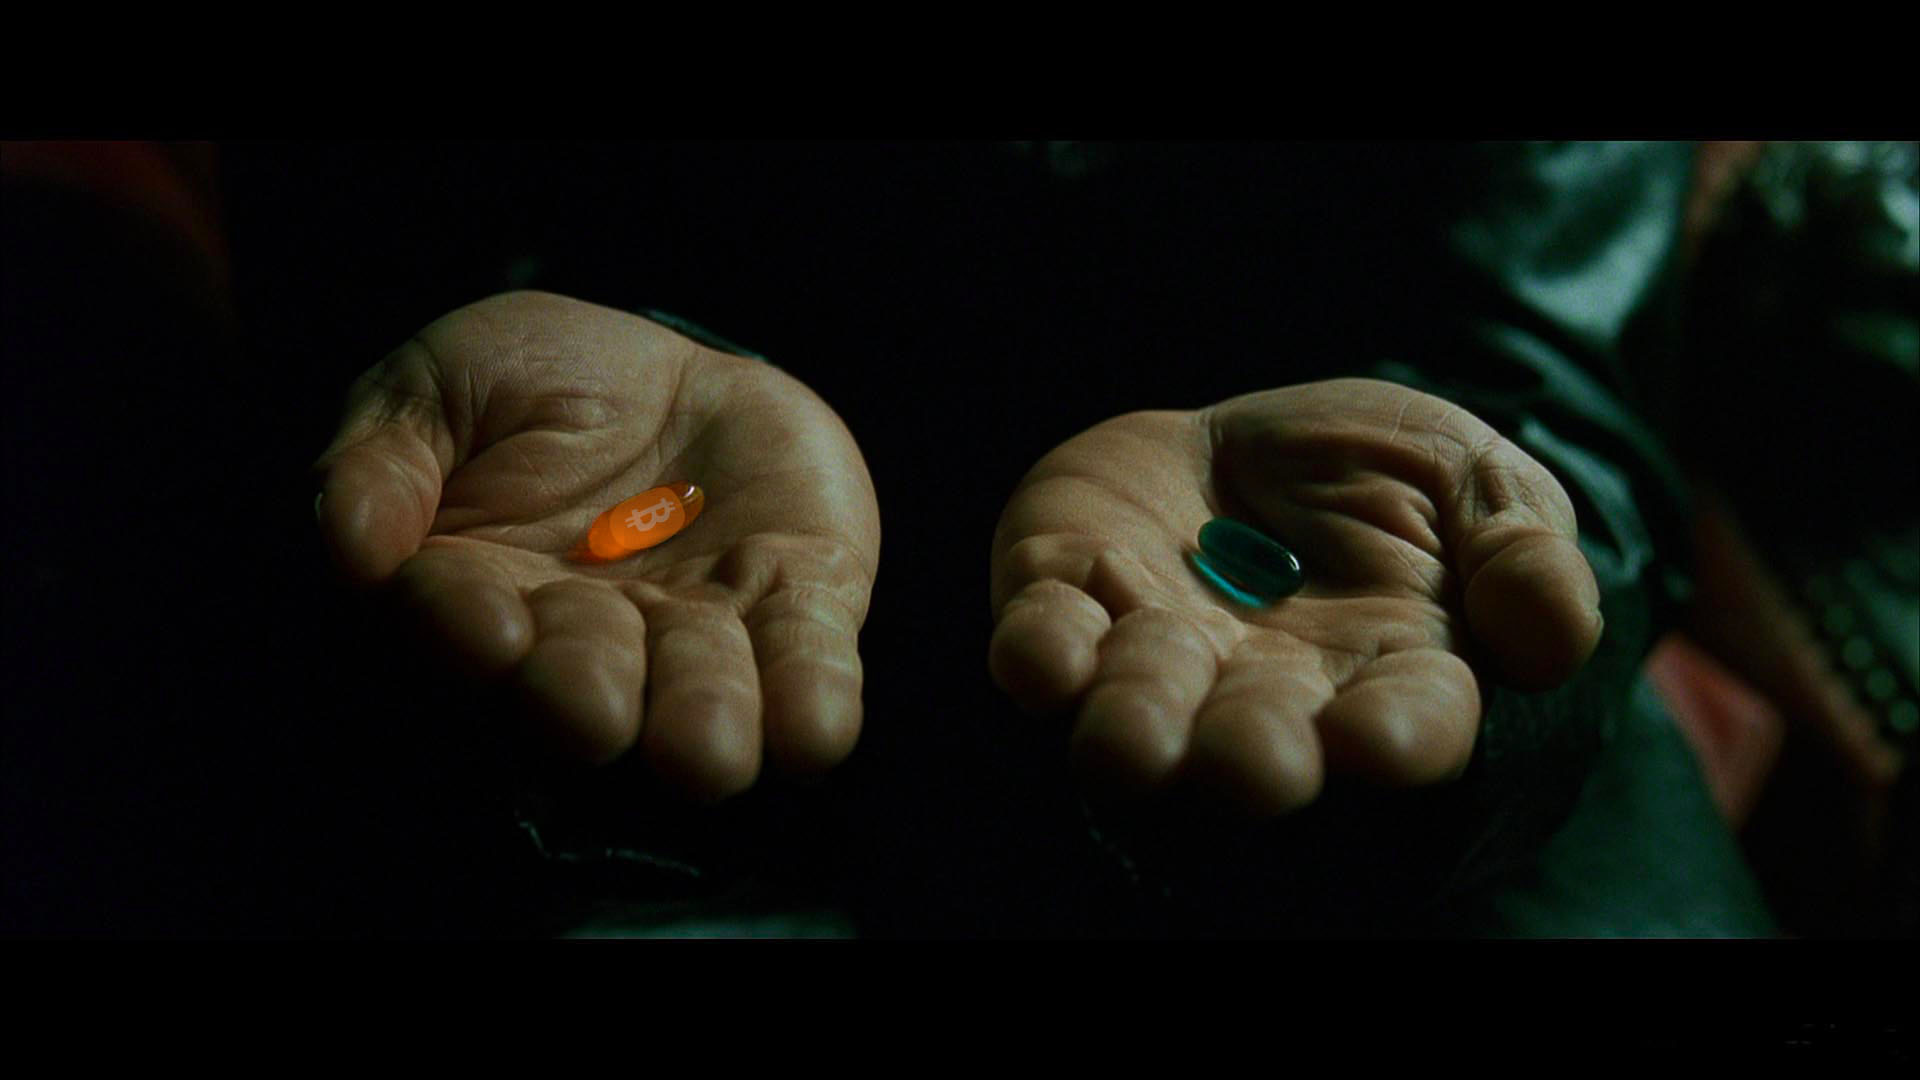
\includegraphics{assets/images/bitcoin-orange-pill.jpg}
  \caption*{Remember: All I'm offering is the truth. Nothing more.}
  \label{fig:bitcoin-orange-pill}
\end{figure}

%
% [Morpheus]: https://en.wikipedia.org/wiki/Red_pill_and_blue_pill#The_Matrix_(1999)
% [this question]: https://twitter.com/arjunblj/status/1050073234719293440
%
% <!-- Internal -->
% [chapter1]: {{ 'bitcoin/lessons/ch1-00-philosophy' | absolute_url }}
% [chapter2]: {{ 'bitcoin/lessons/ch2-00-economics' | absolute_url }}
% [chapter3]: {{ 'bitcoin/lessons/ch3-00-technology' | absolute_url }}
%
% <!-- Wikipedia -->
% [alice]: https://en.wikipedia.org/wiki/Alice%27s_Adventures_in_Wonderland
% [carroll]: https://en.wikipedia.org/wiki/Lewis_Carroll

\part{Philosophy}
\label{ch:philosophy}

% \blockquote{
% The mouse looked at her rather inquisitively, and seemed to her to wink with one
% of its little eyes, but it said nothing.
% }
%
% \newthought{Looking at Bitcoin} superficially, one might conclude that it is slow, wasteful,
% unnecessarily redundant, and overly paranoid. Looking at Bitcoin inquisitively,
% one might find out that things are not as they seem at first glance.

Bitcoin has a way of taking your assumptions and turning them on their heads.
After a while, just when you were about to get comfortable again, Bitcoin will
smash through the wall like a bull in a china shop and shatter your assumptions
once more.

\begin{figure}
  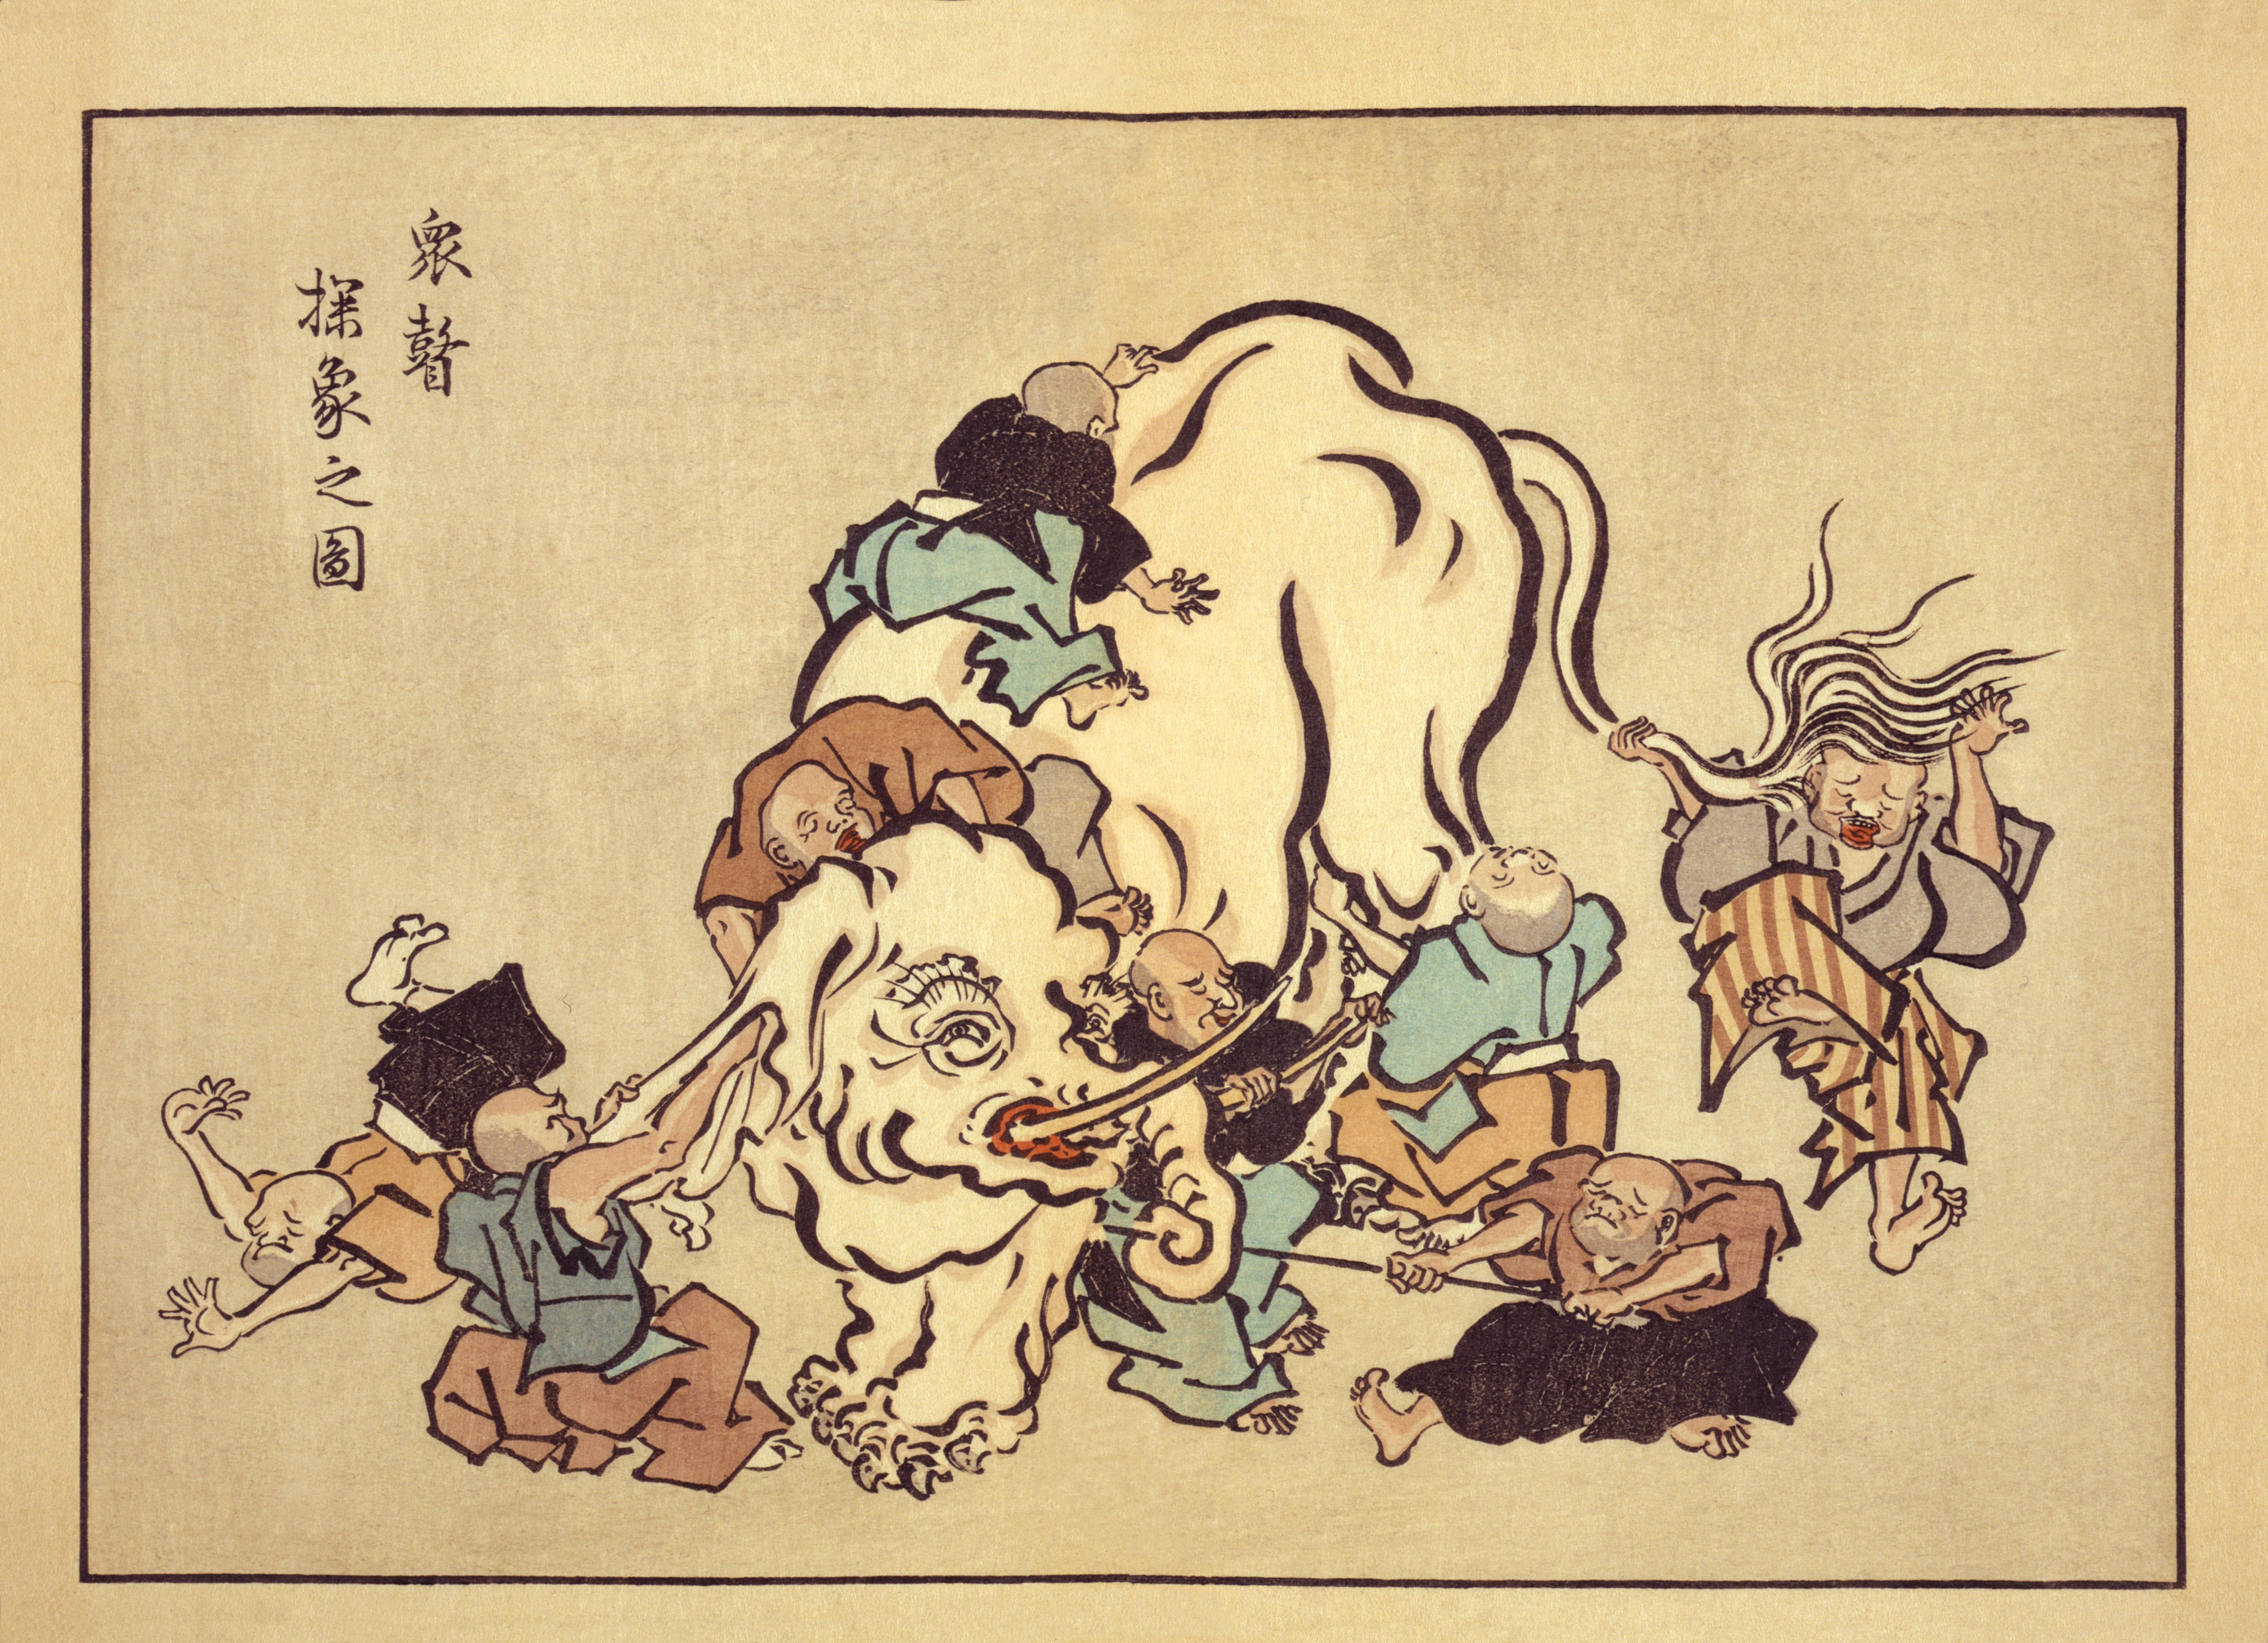
\includegraphics{assets/images/blind-monks.jpg}
  \caption{Blind monks examining the Bitcoin bull}
  \label{fig:blind-monks}
\end{figure}

Bitcoin is a child of many disciplines. Like blind monks examining an elephant,
everyone who approaches this novel technology does so from a different angle.
And everyone will come to different conclusions about the nature of the beast.

The following lessons are about some of my assumptions which Bitcoin shattered,
and the conclusions I arrived at. Philosophical questions of immutability,
scarcity, locality, and identity are explored in the first four lessons.

TODO: Lesson List
% 

Lesson 5 explores how Bitcoin's origin story is not only fascinating but
absolutely essential for a leaderless system. The last two lessons of this
chapter explore the power of free speech and the limits of our individual
knowledge, reflected by the surprising depth of the Bitcoin rabbit hole.

I hope that you will find the world of Bitcoin as educational, fascinating and
entertaining as I did and still do. I invite you to follow the white rabbit and
explore the depths of this rabbit hole. Now hold on to your pocket watch, pop
down, and enjoy the fall.

\chapter{Immutability and Change}
\label{les:1}

\begin{chapquote}{Alice}
\enquote{I wonder if I've been changed in the night. Let me think. Was I the same when I
got up this morning? I almost think I can remember feeling a little different.
But if I'm not the same, the next question is `Who in the world am I?' Ah,
that's the great puzzle!}
\end{chapquote}

Bitcoin is inherently hard to describe. It is a \textit{new thing}, and any
attempt to draw a comparison to previous concepts -- be it by calling
it digital gold or the internet of money -- is bound to fall short of
the whole. Whatever your favorite analogy might be, two aspects of
Bitcoin are absolutely essential: decentralization and immutability.

\paragraph{}
One way to think about Bitcoin is as an automated social contract\footnote{Hasu,
Unpacking Bitcoin's Social Contract~\cite{social-contract}}. The software is
just one piece of the puzzle, and hoping to change Bitcoin by changing the
software is an exercise in futility. One would have to convince the rest of the
network to adopt the changes, which is more a psychological effort than a
software engineering one.

\paragraph{}
The following might sound absurd at first, like so many other things in
this space, but I believe that it is profoundly true nonetheless: You
won't change Bitcoin, but Bitcoin will change you.

\begin{quotation}\begin{samepage}
\enquote{Bitcoin will change us more than we will change it.}
\begin{flushright} -- Marty Bent\footnote{Tales From the Crypt~\cite{tftc21}}
\end{flushright}\end{samepage}\end{quotation}

It took me a long time to realize the profundity of this. Since Bitcoin
is just software and all of it is open-source, you can simply change
things at will, right? Wrong. \textit{Very} wrong. Unsurprisingly, Bitcoin's
creator knew this all too well.

\begin{quotation}\begin{samepage}
\enquote{The nature of Bitcoin is such that once version 0.1 was released, the core
design was set in stone for the rest of its lifetime.}
\begin{flushright} -- Satoshi Nakamoto\footnote{BitcoinTalk forum post: `Re:
Transactions and Scripts\ldots'~\cite{satoshi-set-in-stone}}
\end{flushright}\end{samepage}\end{quotation}

Many people have attempted to change Bitcoin's nature. So far all of
them have failed. While there is an endless sea of forks and altcoins,
the Bitcoin network still does its thing, just as it did when the first
node went online. The altcoins won't matter in the long run. The forks
will eventually starve to death. Bitcoin is what matters. As long as our
fundamental understanding of mathematics and/or physics doesn't change,
the Bitcoin honeybadger will continue to not care.

\begin{quotation}\begin{samepage}
\enquote{Bitcoin is the first example of a new form of life. It lives and
breathes on the internet. It lives because it can pay people to keep
it alive. [\ldots] It can't be changed. It can't be argued with. It
can't be tampered with. It can't be corrupted. It can't be stopped.
[\ldots] If nuclear war destroyed half of our planet, it would continue
to live, uncorrupted.}
\begin{flushright} -- Ralph Merkle\footnote{DAOs, Democracy and
Governance,~\cite{merkle-dao}}
\end{flushright}\end{samepage}\end{quotation}

The heartbeat of the Bitcoin network will outlast all of ours.

~

Realizing the above changed me way more than the past blocks of the Bitcoin
blockchain ever will. It changed my time preference, my understanding of
economics, my political views, and so much more. Hell, it is even changing
people's diets\footnote{Inside the World of the Bitcoin
Carnivores,~\cite{carnivores}}. If all of this sounds crazy to you, you're in
good company. All of this is crazy, and yet it is happening.

~

\paragraph{Bitcoin taught me that it won't change. I will.}

% ---
%
% #### Through the Looking-Glass
%
% - [Bitcoin's Gravity: How idea-value feedback loops are pulling people in][gravity]
% - [Lesson 18: Move slowly and don't break things][lesson18]
%
% #### Down the Rabbit Hole
%
% - [Unpacking Bitcoin's Social Contract][automated social contract]: A framework for skeptics by Hasu
% - [DAOs, Democracy and Governance][Ralph Merkle] by Ralph C. Merkle
% - [Marty's Bent][bent]: A daily newsletter highlighting signal in Bitcoin by Marty Bent
% - [Technical Discussion on Bitcoin's Transactions and Scripts][Satoshi Nakamoto] by Satoshi Nakamoto, Gavin Andresen, and others
% - [Inside the World of the Bitcoin Carnivores][carnivores]: Why a small community of Bitcoin users is eating meat exclusively by Jordan Pearson
% - [Tales From the Crypt][tftc] hosted by Marty Bent
%
% <!-- Internal -->
% [gravity]: 
% [lesson18]: {{ 'bitcoin/lessons/ch3-18-move-slowly-and-dont-break-things' | absolute_url }}
%
% <!-- Further Reading -->
% [automated social contract]: https://medium.com/@hasufly/bitcoins-social-contract-1f8b05ee24a9
% [carnivores]: https://motherboard.vice.com/en_us/article/ne74nw/inside-the-world-of-the-bitcoin-carnivores
% [tftc]: https://tftc.io/tales-from-the-crypt/
% [bent]: https://tftc.io/martys-bent/
%
% <!-- Quotes -->
% [Ralph Merkle]: http://merkle.com/papers/DAOdemocracyDraft.pdf
% [Satoshi Nakamoto]: https://bitcointalk.org/index.php?topic=195.msg1611#msg1611
%
% <!-- Twitter People -->
% [Marty Bent]: https://twitter.com/martybent
%
% <!-- Wikipedia -->
% [alice]: https://en.wikipedia.org/wiki/Alice%27s_Adventures_in_Wonderland
% [carroll]: https://en.wikipedia.org/wiki/Lewis_Carroll


\chapter{ The Scarcity of Scarcity}
\label{les:2}

\begin{chapquote}{Alice}
That's quite enough - I hope I sha'n't grow any more...
\end{chapquote}

In general, the advance of technology seems to make things more abundant. More
and more people are able to enjoy what previously have been luxurious goods.
Soon, we will all live like kings. Most of us already do. As Peter Diamandis
wrote in Abundance\cite{abundance}: ``Technology is a resource-liberating
mechanism. It can make the once scarce the now abundant.''

Bitcoin, an advanced technology in itself, breaks this trend and creates
a new commodity which is truly scarce. Some even argue that it is one of
the scarcest things in the universe. The supply can't be inflated, no
matter how much effort one chooses to expend towards creating more.

\begin{chapquote}{\cite{bitcoinstandard-pres}}
``Only two things are genuinely scarce: time and
bitcoin.''
\end{chapquote}

Paradoxically, it does so by a mechanism of copying. Transactions are
broadcast, blocks are propagated, the distributed ledger is --- well,
you guessed it --- distributed. All of these are just fancy words for
copying. Heck, Bitcoin even copies itself onto as many computers as it
can, by incentivizing individual people to run full nodes and mine new
blocks.

All of this duplication wonderfully works together in a concerted effort
to produce scarcity.

In a time of abundance, Bitcoin taught me what real scarcity is.

% ---
%
% #### Through the Looking-Glass
%
% - [Lesson 14: Sound money][lesson14]
%
% #### Down the Rabbit Hole
%
% - [The Bitcoin Standard: The Decentralized Alternative to Central Banking][bitcoin-standard]
% - [Abundance: The Future Is Better Than You Think][Abundance] by Peter Diamandis
% - [Presentation on The Bitcoin Standard][bitcoin-standard-presentation] by Saifedean Ammous
% - [Modeling Bitcoin's Value with Scarcity][planb-scarcity] by PlanB
% - 🎧 [Misir Mahmudov on the Scarcity of Time & Bitcoin][tftc60] TFTC #60 hosted by Marty Bent
% - 🎧 [PlanB – Modelling Bitcoin's digital scarcity through stock-to-flow techniques][slp67] SLP #67 hosted by Stephan Livera
%
% <!-- Through the Looking-Glass -->
% [lesson14]: {{ 'bitcoin/lessons/ch2-14-sound-money' | absolute_url }}
%
% <!-- Down the Rabbit Hole -->
% [Abundance]: https://www.diamandis.com/abundance
% [bitcoin-standard]: http://amzn.to/2L95bJW
% [bitcoin-standard-presentation]: https://www.bayernlb.de/internet/media/de/ir/downloads_1/bayernlb_research/sonderpublikationen_1/bitcoin_munich_may_28.pdf
% [planb-scarcity]: https://medium.com/@100trillionUSD/modeling-bitcoins-value-with-scarcity-91fa0fc03e25
% [tftc60]: https://anchor.fm/tales-from-the-crypt/episodes/Tales-from-the-Crypt-60-Misir-Mahmudov-e3aibh
% [slp67]: https://stephanlivera.com/episode/67
%
% <!-- Wikipedia -->
% [alice]: https://en.wikipedia.org/wiki/Alice%27s_Adventures_in_Wonderland
% [carroll]: https://en.wikipedia.org/wiki/Lewis_Carroll

\chapter{Replicação e Localidade}
\label{les:3}

\begin{chapquote}{Lewis Carroll, \textit{Alice no País das Maravilhas}}
Em seguida uma voz irada, do Coelho: \enquote{Pat, Pat! onde você está?}
\end{chapquote}

Deixando a mecânica quântica de lado, a localidade não é um problema no mundo físico. A questão \textit{\enquote{Onde está X?}} Pode ser respondida de forma significativa, não importa se X é uma pessoa ou um objeto. No mundo digital, a pergunta do \textit{onde} já é mais complicada, mas não impossível de responder. Onde estão seus e-mails realmente? Uma resposta não muito boa seria \enquote{na nuvem} que nada mais é que o computador de outra pessoa. Ainda assim, se você quisesse rastrear cada dispositivo de armazenamento que contém seus e-mails, você poderia, em teoria, localizá-los.

Com o bitcoin, a pergunta do \enquote{onde} é \textit{realmente} complicada. Onde, exatamente, estão seus bitcoins?

\begin{quotation}\begin{samepage}
\enquote{Abri os olhos, olhei em volta e fiz a pergunta inevitável, tradicional e lamentavelmente banal do pós-operatório: "Onde estou?"}
\begin{flushright} -- Daniel Dennett\footnote{Daniel Dennett, \textit{Where Am I?}~\cite{where-am-i}}
\end{flushright}\end{samepage}\end{quotation}

O problema é duplo. Primeiro, o livro-razão distribuído é distribuído por replicação completa, o que significa que ele está em toda parte. Em segundo lugar, não existem bitcoins. Não apenas fisicamente, mas \textit{tecnicamente}.

O Bitcoin rastreia um conjunto de saídas de transações não gastas, sem nunca ter que se referir a uma entidade que represente um bitcoin. A existência de um bitcoin é baseada observando-se o conjunto de saídas de transações não gastas e chamando cada entrada com 100 milhões de unidades básicas de bitcoin.

\begin{quotation}\begin{samepage}
\enquote{Onde está, neste momento, em trânsito? [...] primeiro, não há bitcoins. Simplesmente não existem. Eles não existem. Existem entradas em um livro-razão que é compartilhado [...] Eles não existem em nenhum local físico. O livro-razão existe em todos os locais físicos, essencialmente. A geografia não faz sentido neste mundo --- não vai ajudá-lo a descobrir a sua política aqui.}
\begin{flushright} -- Peter Van Valkenburgh\footnote{Peter Van Valkenburgh on the \textit{What Bitcoin Did} podcast, episode 49 \cite{wbd049}}
\end{flushright}\end{samepage}\end{quotation}

Então, o que você realmente possui quando diz \textit{\enquote{Eu tenho um bitcoin}} se não há bitcoins? Bem, lembra de todas essas palavras estranhas que você foi forçado a escrever quando usou uma carteira? Acontece que essas palavras mágicas são o que você realmente possui: um feitiço mágico \footnote{The Magic Dust of Cryptography: Como a informação digital está mudando nossa sociedade \cite{gigi:magic-spell}} que pode ser usado para adicionar algumas entradas ao livro-razão público --- as chaves para \enquote{mover} alguns bitcoins. É por isso que, para todos os efeitos, suas chaves privadas \textit{são} seus bitcoins. Se você acha que estou inventando tudo isso, sinta-se à vontade para me enviar suas chaves privadas.

\paragraph{O Bitcoin me ensinou que localidade é um negócio complicado.}

% ---
%
% #### Through the Looking-Glass
%
% - [The Magic Dust of Cryptography: How digital information is changing our society][a magic spell]
%
% #### Down the Rabbit Hole
%
% - [Where Am I?][Daniel Dennett] by Daniel Dennett
% - 🎧 [Peter Van Valkenburg on Preserving the Freedom to Innovate with Public Blockchains][wbd049] WBD #49 hosted by Peter McCormack
%
% <!-- Through the Looking-Glass -->
% [a magic spell]: 
%
% <!-- Down the Rabbit Hole -->
% [Daniel Dennett]: https://www.lehigh.edu/~mhb0/Dennett-WhereAmI.pdf
% [1st Amendment]: https://en.wikipedia.org/wiki/First_Amendment_to_the_United_States_Constitution
% [wbd049]: https://www.whatbitcoindid.com/podcast/coin-centers-peter-van-valkenburg-on-preserving-the-freedom-to-innovate-with-public-blockchains
%
% <!-- Wikipedia -->
% [alice]: https://en.wikipedia.org/wiki/Alice%27s_Adventures_in_Wonderland
% [carroll]: https://en.wikipedia.org/wiki/Lewis_Carroll

\chapter{The Problem of Identity}
\label{les:4}

\begin{chapquote}{Lewis Carroll, \textit{Alice in Wonderland}}
  \enquote{Who are you?} said the caterpillar.
\end{chapquote}

Nic Carter, in an homage to Thomas Nagel's treatment of the same
question in regards to a bat, wrote an excellent piece which discusses
the following question: What is it like to be a bitcoin? He
brilliantly shows that open, public blockchains in general, and Bitcoin
in particular, suffer from the same conundrum as the Ship of
Theseus: which Bitcoin is the real Bitcoin?

\begin{quotation}\begin{samepage}
\enquote{Consider just how little persistence Bitcoin's components have. The
entire codebase has been reworked, altered, and expanded such that it
barely resembles its original version. [...] The registry of who
owns what, the ledger itself, is virtually the only persistent trait
of the network [...]
To be considered truly leaderless, you must surrender the easy
solution of having an entity that can designate one chain as the
legitimate one.}
\begin{flushright} -- Nic Carter\footnote{Nic Carter, \textit{What is it like to be a bitcoin?} \cite{bitcoin-identity}}
\end{flushright}\end{samepage}\end{quotation}

It seems like the advancement of technology keeps forcing us to take
these philosophical questions seriously. Sooner or later, self-driving
cars will be faced with real-world versions of the trolley problem,
forcing them to make ethical decisions about whose lives do matter and
whose do not.

Cryptocurrencies, especially since the first contentious hard-fork,
force us to think about and agree upon the metaphysics of identity.
Interestingly, the two biggest examples we have so far have lead to two
different answers. On August 1, 2017, Bitcoin split into two camps. The
market decided that the unaltered chain is the original Bitcoin. One
year earlier, on October 25, 2016, Ethereum split into two camps. The
market decided that the \textit{altered} chain is the original Ethereum.

If properly decentralized, the questions posed by the \textit{Ship of Theseus}
will have to be answered in perpetuity for as long as these networks of
value-transfer exist.

\paragraph{Bitcoin taught me that decentralization contradicts identity.}

% ---
%
% #### Down the Rabbit Hole
%
% - [What Is It Like to be a Bat?][in regards to a bat] by Thomas Nagel
% - [What is it like to be a bitcoin?] by Nic Carter
% - [Ship of Theseus], [trolley problem] on Wikipedia
%
% [in regards to a bat]: https://en.wikipedia.org/wiki/What_Is_it_Like_to_Be_a_Bat%3F
% [What is it like to be a bitcoin?]: https://medium.com/s/story/what-is-it-like-to-be-a-bitcoin-56109f3e6753
% [Ship of Theseus]: https://en.wikipedia.org/wiki/Ship_of_Theseus
% [trolley problem]: https://en.wikipedia.org/wiki/Trolley_problem
%
% <!-- Wikipedia -->
% [alice]: https://en.wikipedia.org/wiki/Alice%27s_Adventures_in_Wonderland
% [carroll]: https://en.wikipedia.org/wiki/Lewis_Carroll

\chapter{Uma concepção imaculada}
\label{les:5}

\begin{chapquote}{Lewis Carroll, \textit{Alice no País das Maravilhas}}
\enquote{Suas cabeças se foram, para servi-la, Majestade}, os soldados gritaram em resposta\ldots
\end{chapquote}

Todo mundo adora uma boa história de origem. A história de origem do Bitcoin é fascinante, e os detalhes dela são mais importantes do que se possa pensar quando sabemos pela primeira vez. Quem é Satoshi Nakamoto? Ele era uma pessoa ou um grupo de pessoas? Ele era ela? Seria um alien viajando no tempo ou IA avançada? Deixando de lado as teorias estranhas, provavelmente nunca saberemos. E isso é importante.

O Satoshi escolheu ser anônimo. Ele plantou a semente do Bitcoin. Ele ficou por aqui por tempo suficiente para garantir que a rede não morresse quando estava engatinhando. E então ele desapareceu.

O que pode parecer um golpe estranho de anonimato é realmente crucial para um sistema verdadeiramente descentralizado. Sem controle centralizado. Nenhuma autoridade centralizada. Nenhum inventor. Ninguém para processar, torturar, chantagear ou extorquir. Uma concepção imaculada de tecnologia.

\begin{quotation}\begin{samepage}
\enquote{Uma das melhores coisas que Satoshi fez foi desaparecer.}
\begin{flushright} -- Jimmy Song\footnote{Jimmy Song, \textit{Por que o Bitcoin é Diferente} \cite{bitcoin-different}}
\end{flushright}\end{samepage}\end{quotation}

\newpage

Desde o nascimento do Bitcoin, milhares de outras criptomoedas foram criadas. Nenhum desses clones compartilha sua história de origem. Se você quiser substituir o Bitcoin, terá que transcender sua história de origem. Em uma guerra de ideias, as narrativas ditam a sobrevivência.

\begin{quotation}\begin{samepage}
\enquote{O ouro foi transformado pela primeira vez em joias e usado para troca há mais de 7.000 anos. O brilho cativante do ouro o levou a ser considerado um presente
dos deuses.}
\begin{flushright} Austrian Mint\footnote{The Austrian Mint, \textit{Gold: The Extraordinary Metal} \cite{gold-gift-gods}}
\end{flushright}\end{samepage}\end{quotation}

Como o ouro nos tempos antigos, o Bitcoin pode ser considerado um presente dos deuses. Ao contrário do ouro, as origens dos Bitcoins são muito humanas. E desta vez, sabemos quem são os deuses do desenvolvimento e da manutenção: pessoas de todo o mundo, anônimas ou não.

\paragraph{O Bitcoin me ensinou que narrativas são importantes.}

% ---
%
% #### Down the Rabbit Hole
%
% - [Why Bitcoin is different][Jimmy Song] by Jimmy Song
% - [Gold: The Extraordinary Metal] by the Austrian Mint
%
% <!-- Down the Rabbit Hole -->
% [Jimmy Song]: https://medium.com/@jimmysong/why-bitcoin-is-different-e17b813fd947
% [Gold: The Extraordinary Metal]: https://www.muenzeoesterreich.at/eng/discover/for-investors/gold-the-extraordinary-metal
%
% <!-- Wikipedia -->
% [alice]: https://en.wikipedia.org/wiki/Alice%27s_Adventures_in_Wonderland
% [carroll]: https://en.wikipedia.org/wiki/Lewis_Carroll

\chapter{The Power of Free Speech}
\label{les:6}

\begin{chapquote}{Lewis Carroll, \textit{Alice in Wonderland}}
``I beg your pardon?'' said the mouse, frowning, but very politely, ``did you speak?''
\end{chapquote}

Bitcoin is an idea. An idea which, in its current form, is the
manifestation of a machinery purely powered by text. Every aspect of
Bitcoin is text: The whitepaper is text. The software which is run by
its nodes is text. The ledger is text. Transactions are text. Public and
private keys are text. Every aspect of Bitcoin is text, and thus
equivalent to speech.

\begin{quotation}
``Congress shall make no law respecting an establishment of religion,
or prohibiting the free exercise thereof; or abridging the freedom of
speech, or of the press; or the right of the people peaceably to
assemble, and to petition the Government for a redress of grievances.''
\flushright -- First Amendment to the U.S. Constitution
\end{quotation}
% > <cite>[First Amendment to the United States Constitution][1st Amendment]</cite>

Although the final battle of the [Crypto Wars] has not been fought yet,
it will be very difficult to criminalize an idea, let alone an idea
which is based on the exchange of text messages. Every time a government
tries to outlaw text or speech, we slip down a path of absurdity which
inevitably leads to abominations like [illegal numbers] and [illegal
primes].

As long as there is a part of the world where speech is free as in
\textit{freedom}, Bitcoin is unstoppable.

\begin{quotation}
``There is no point in any Bitcoin transaction that Bitcoin ceases to be
\textbf{text}. It is \textbf{all text}, all the time. [...] Bitcoin is
\textbf{text}. Bitcoin is \textbf{speech}. It cannot be regulated in a free
country like the USA with guaranteed inalienable rights and a First Amendment
that explicitly excludes the act of publishing from government oversight.''
\end{quotation}
% > <cite>[Beautyon]</cite>

\paragraph{Bitcoin taught me that in a free society, free speech and free software
are unstoppable.}

% ---
%
% #### Through the Looking-Glass
%
% - [The Magic Dust of Cryptography: How digital information is changing our society][a magic spell]
%
% #### Down the Rabbit Hole
%
% - [Why America can't regulate Bitcoin][Beautyon] by Beautyon
% - [First Amendment to the United States Constitution][1st Amendment], [Crypto Wars], [illegal numbers], [illegal primes] on Wikipedia
%
% <!-- Through the Looking-Glass -->
% [a magic spell]: 
%
% <!-- Down the Rabbit Hole -->
% [1st Amendment]: https://en.wikipedia.org/wiki/First_Amendment_to_the_United_States_Constitution
% [Crypto Wars]: https://en.wikipedia.org/wiki/Crypto_Wars
% [illegal numbers]: https://en.wikipedia.org/wiki/Illegal_number
% [illegal primes]: https://en.wikipedia.org/wiki/Illegal_prime
% [Beautyon]: https://hackernoon.com/why-america-cant-regulate-bitcoin-8c77cee8d794
%
% <!-- Wikipedia -->
% [alice]: https://en.wikipedia.org/wiki/Alice%27s_Adventures_in_Wonderland
% [carroll]: https://en.wikipedia.org/wiki/Lewis_Carroll

\chapter{ The Limits of Knowledge}
\label{les:7}

\begin{chapquote}{Lewis Carroll, \textit{Alice in Wonderland}}
``Down, down, down. Would the fall never come to an end?''
\end{chapquote}

Getting into Bitcoin is a humbling experience. I thought that I knew
things. I thought that I was educated. I thought that I knew my computer
science, at the very least. I studied it for years, so I have to know
everything about digital signatures, hashes, encryption, operational
security, and networks, right?

Wrong.

Learning all the fundamentals which make Bitcoin work is hard.
Understanding all of them deeply is borderline impossible.

\begin{quotation}
``No one has found the bottom of the Bitcoin rabbit hole.''
\end{quotation}
% > <cite>[Jameson Lopp]</cite>

My list of books to read keeps expanding way quicker than I could
possibly read them. The list of papers and articles to read is virtually
endless. There are more podcasts on all of these topics than I could
ever listen to. It truly is humbling. Further, Bitcoin is evolving and
it's almost impossible to stay up-to-date with the accelerating rate of
innovation. The dust of the first layer hasn't even settled yet, and
people have already built the second layer and are working on the third.

Bitcoin taught me that I know very little about almost anything. It
taught me that this rabbit hole is bottomless.

% ---
%
% #### Down the Rabbit Hole
%
% - [Bitcoin Literature] by the Satoshi Nakamoto Institute
% - [Bitcoin Information & Resources][lopp-resources] by Jameson Lopp
% - [Educational Resources][bitcoin-only] by Bitcoin Only
%
% <!-- Twitter -->
% [Jameson Lopp]: https://twitter.com/lopp/status/1061415918616698881
%
% <!-- Down the Rabbit Hole -->
% [lopp-resources]: https://www.lopp.net/bitcoin-information.html
% [bitcoin-only]: https://bitcoin-only.com/#learning
% [Bitcoin Literature]: https://nakamotoinstitute.org/literature/
%
% <!-- Wikipedia -->
% [alice]: https://en.wikipedia.org/wiki/Alice%27s_Adventures_in_Wonderland
% [carroll]: https://en.wikipedia.org/wiki/Lewis_Carroll


\chapter{Economics}
\label{ch:economics}

\begin{chapquote}{Lewis Carroll, \textit{Alice in Wonderland}}
``A large rose tree stood near the entrance of the garden: the roses on it were
white, but there were three gardeners at it, busily painting them red. This
Alice thought a very curious thing...''
\end{chapquote}

\newthought{Money doesn’t grow on trees.} To believe that it does is foolish, and our
parents make sure that we know about that by repeating this saying like a
mantra. We are encouraged to use money wisely, to not spend it frivolously,
and to save it in good times to help us through the bad. Money, after all,
does not grow on trees.

Bitcoin taught me more about money than I ever thought I would need to know.
Through it, I was forced to explore the history of money, banking, various
schools of economic thought, and many other things. The quest to understand
Bitcoin lead me down a plethora of paths, some of which I try to explore in
this series.

In the first seven lessons some of the philosophical questions Bitcoin touches
on were discussed. The next seven lessons will take a closer look at money and
economics.

\TODO{Lesson List}
% 

Again, I will only be able to scratch the surface. Bitcoin is not only
ambitious, but also broad and deep in scope, making it impossible to cover all
relevant topics in a single lesson, essay, article, or book. I  doubt if it is
even possible at all.

\newthought{Bitcoin is a new form of money}, which makes learning about
economics paramount to understanding it. Dealing with the nature of human action
and the interactions of economic agents, economics is probably one of the
largest and fuzziest pieces of the Bitcoin puzzle.

Again, these lessons are an exploration of the various things I have learned
from Bitcoin. They are a personal reflection of my journey down the rabbit hole.
Having no background in economics, I am definitely out of my comfort zone and
especially aware that any understanding I might have is incomplete. I will do my
best to outline what I have learned, even at the risk of making a fool out of
myself. After all, I am still trying to answer the question: ``What have you
learned from Bitcoin?''

\begin{marginfigure}%
  
\includegraphics{assets/images/the-tweet.png}
  \caption{What have you learned from Bitcoin?}
  \label{fig:tweet}
\end{marginfigure}

After seven lessons examined through the lens of philosophy, let’s use the lens
of economics to look at seven more. Economy class is all I can offer this time.
Final destination: \textit{sound money}.

% [the question]: https://twitter.com/arjunblj/status/1050073234719293440

\chapter{Ignorância financeira}
\label{les:8}

\begin{chapquote}{Lewis Carroll, \textit{Alice no País das Maravilhas}}
\enquote{Ela iria pensar que eu sou uma garotinha ignorante por perguntar! Não, não vou perguntar nunca. Talvez eu possa ver o nome escrito em algum lugar..}
\end{chapquote}

Uma das coisas mais surpreendentes, para mim, foi a quantidade de finanças, economia e psicologia necessária para obter uma compreensão do que, à primeira vista, parece ser um sistema puramente \textit{técnico} --- uma rede de computadores. Parafraseando um baixinho com pés peludos: \enquote{É um negócio perigoso, Frodo, pisar no Bitcoin. Você lê o whitepaper e, se não se controlar, não há como saber para onde pode ser levado.}

Para entender um novo sistema monetário, você precisa se familiarizar com o antigo. Comecei a perceber logo que a quantidade de educação financeira que desfrutava no sistema educacional era essencialmente \textit{zero}.

\paragraph{}
Como uma criança de cinco anos, comecei a me fazer muitas perguntas: Como funciona o sistema bancário? Como funciona o mercado de ações? O que é moeda fiduciária? O que é dinheiro \textit{normal}? Por que existe tanta dívida? \footnote{\url{https://www.usdebtclock.org/}} Quanto dinheiro é impresso e quem decide isso?

\newpage

Depois de um leve pânico sobre a extensão da minha ignorância, encontrei segurança ao perceber que estava em boa companhia.

\begin{quotation}\begin{samepage}
\enquote{Não é irônico que o Bitcoin tenha me ensinado mais sobre dinheiro do que todos esses anos que passei trabalhando para instituições financeiras?\ldots incluindo a minha carreira em um banco central.}
\begin{flushright} -- Aaron\footnote{Aaron (\texttt{@aarontaycc}, \texttt{@fiatminimalist}), tweet de 12 de dezembro de 2018~\cite{aarontaycc-tweet}}
\end{flushright}\end{samepage}\end{quotation}

\begin{quotation}\begin{samepage}
\enquote{Aprendi mais sobre finanças, economia, tecnologia, criptografia, psicologia humana, política, teoria dos jogos, legislação e sobre mim mesmo nos últimos três meses de cripto do que nos últimos três anos e meio de faculdade.}
\begin{flushright} -- Dunny\footnote{Dunny (\texttt{@BitcoinDunny}), tweet de 28 de Novembro de 2017~\cite{bitcoindunny-tweet}}
\end{flushright}\end{samepage}\end{quotation}

Estas são apenas duas das muitas confissões em todo o Twitter. \footnote{Veja \url{http://bit.ly/btc-learned} para mais confissões no Twitter.} O Bitcoin, como foi explorado na Lição \ref{les: 1}, é uma coisa viva. Mises argumentou que a economia também é uma coisa viva. E, como todos sabemos por experiência pessoal, as coisas vivas são inerentemente difíceis de entender.

\begin{quotation}\begin{samepage}
\enquote{Um sistema científico é apenas uma estação em uma busca interminável pelo conhecimento. É necessariamente afetado pela insuficiência inerente a todo esforço humano. Mas reconhecer esses fatos não significa que a economia atual esteja atrasada. Significa apenas que a economia é uma coisa viva --- e viver implica imperfeição e mudança.}
\begin{flushright} -- Ludwig von Mises\footnote{Ludwig von Mises, \textit{Ação Humana}
\cite{human-action}}
\end{flushright}\end{samepage}\end{quotation}

Todos nós lemos sobre várias crises financeiras no noticiário, nos perguntamos como funcionam esses grandes resgates e ficamos intrigados com o fato de que ninguém parece jamais ser responsabilizado pelos danos, que estão na casa dos trilhões. Ainda estou confuso, mas pelo menos estou começando a ter um vislumbre do que está acontecendo no mundo das finanças.

Algumas pessoas chegam ao ponto de atribuir a ignorância geral sobre esses tópicos à ignorância intencional e sistêmica. Embora história, física, biologia, matemática e línguas façam parte de nossa educação, o mundo do dinheiro e das finanças, surpreendentemente, só é explorado superficialmente, se é que é explorado. Eu me pergunto se as pessoas ainda estariam dispostas a acumular tantas dívidas como fazem atualmente se todos fossem educados em finanças pessoais e no funcionamento do dinheiro e das dívidas. Então eu me pergunto: quantas camadas de alumínio formam um chapéu de papel-alumínio eficaz. Provavelmente três.

\begin{quotation}\begin{samepage}
\enquote{Essas crises, esses resgates, não são acidentes. E também não é por acaso que não há educação financeira na escola. [...] É premeditado. Assim como antes da Guerra Civil, era ilegal educar um escravo, não podemos aprender sobre o dinheiro na escola.}
\begin{flushright} -- Robert Kiyosaki\footnote{Robert Kiyosaki, \textit{Por Que o Rico Está Ficando Mais Rico}\cite{robert-kiyosaki}}
\end{flushright}\end{samepage}\end{quotation}

Como na história de O mágico de Oz, somos orientados a não dar atenção ao homem por trás da cortina. Ao contrário do O Mágico de Oz, agora temos magia real \footnote{\url{http://bit.ly/btc-wizardry}}: uma rede de transferência de valor aberta, resistente à censura e sem fronteiras. Não há cortina, e a magia é visível para qualquer um. \footnote{\url{https://github.com/bitcoin/bitcoin}}

\paragraph{Bitcoin me ensinou a olhar atrás da cortina e enfrentar minha ignorância financeira.}

% ---
%
% #### Down the Rabbit Hole
%
% - [Human Action][Ludwig von Mises] by Ludwig von Mises
% - [Why the Rich are Getting Richer][Robert Kiyosaki] by Robert Kiyosaki
%
% [real wizardry]: https://external-preview.redd.it/8d03MWWOf2HIyKrT8ThBGO4WFv-u25JaYqhbEO9b1Sk.jpg?width=683&auto=webp&s=dc5922d84717c6a94527bafc0189fd4ca02a24bb
% [visible to anyone]: https://github.com/bitcoin/bitcoin
%
% <!-- Wikipedia -->
% [alice]: https://en.wikipedia.org/wiki/Alice%27s_Adventures_in_Wonderland
% [carroll]: https://en.wikipedia.org/wiki/Lewis_Carroll

\chapter{Lesson 9: Inflation}
\label{les:9}

\begin{chapquote}{Lewis Carroll, \textit{Alice in Wonderland}}
``My dear, here we must run as fast as we can, just to stay in place. And if you
wish to go anywhere you must run twice as fast as that.''
\end{chapquote}

Trying to understand monetary inflation, and how a non-inflationary
system like Bitcoin might change how we do things, was the starting
point of my venture into economics. I knew that inflation was the rate
at which new money was created, but I didn't know too much beyond that.

While some economists argue that inflation is a good thing, others argue
that "hard" money which can't be inflated easily --- as we had in the
days of the gold standard --- is essential for a healthy economy.
Bitcoin, having a fixed supply of 21 million, agrees with the latter
camp.

Usually, the effects of inflation are not immediately obvious. Depending
on the inflation rate (as well as other factors) the time between cause
and effect can be several years. Not only that, but inflation affects
different groups of people more than others. As Henry Hazlitt points out
in *Economics in One Lesson*: "The art of economics consists in looking
not merely at the immediate but at the longer effects of any act or
policy; it consists in tracing the consequences of that policy not
merely for one group but for all groups."

One of my personal lightbulb moments was the realization that issuing
new currency --- printing more money --- is a *completely* different
economic activity than all the other economic activities. While real
goods and real services produce real value for real people, printing
money effectively does the opposite: it takes away value from everyone
who holds the currency which is being inflated.

\begin{quotation}
``Mere inflation --- that is, the mere issuance of more money, with the
consequence of higher wages and prices --- may look like the creation
of more demand. But in terms of the actual production and exchange of
real things it is not.''
\end{quotation}
% > <cite>[Henry Hazlitt]</cite>

The destructive force of inflation becomes obvious as soon as a little
inflation turns into *a lot*. If money [hyperinflates], things get ugly
real quick. As the inflating currency falls apart, it will fail to store
value over time and people will rush to get their hands on any goods
which might do.

Another consequence of hyperinflation is that all the money which people
have saved over the course of their life will effectively vanish. The
paper money in your wallet will still be there, of course. But it will
be exactly that: worthless paper.


% 

Money declines in value with so-called "mild" inflation as well. It
just happens slowly enough that most people don't notice the diminishing
of their purchasing power. And once the printing presses are running,
currency can be easily inflated, and what used to be mild inflation
might turn into a strong cup of inflation by the push of a button. As
Friedrich Hayek pointed out in one of his essays, mild inflation usually
leads to outright inflation.

\begin{quotation}
```Mild' steady inflation cannot help --- it can lead only to outright
inflation.''
\end{quotation}
% > <cite>[Friedrich Hayek][inflation cannot help]</cite>

Inflation is particularly devious since it favors those who are closer
to the printing presses. It takes time for the newly created money to
circulate and prices to adjust, so if you are able to get your hands on
more money before everyone else's devaluates you are ahead of the
inflationary curve. This is also why inflation can be seen as a hidden
tax because in the end governments profit from it while everyone else
ends up paying the price.

\begin{quotation}
``I do not think it is an exaggeration to say history is largely a
history of inflation, and usually of inflations engineered by
governments for the gain of governments.''
\end{quotation}
% > <cite>[Friedrich Hayek][history of inflation]</cite>

So far, all government-controlled currencies have eventually been
replaced or have collapsed completely. No matter how small the rate of
inflation, "steady" growth is just another way of saying exponential
growth. In nature as in economics, all systems which grow exponentially
will eventually have to level off or suffer from catastrophic collapse.

"It can't happen in my country," is what you're probably thinking. You
don't think that if you are from Venezuela, which is [currently
suffering][wiki-venezuela] from hyperinflation. With an inflation rate of over 1 million
percent, money is basically worthless.

It might not happen in the next couple of years, or to the particular
currency used in your country. But a glance at the [list of historical
currencies] shows that it will inevitably happen over a long enough period of
time. I remember and used plenty of those listed: the Austrian
schilling, the German mark, the Italian lira, the French franc, the
Irish pound, the Croatian dinar, etc. My grandma even used the
Austro-Hungarian Krone. As time moves on, the currencies [currently in
use] will slowly but surely move to their respective graveyards. They
will hyperinflate or be replaced. They will soon be historical
currencies. We will make them obsolete.

\begin{quotation}
``History has shown that governments will inevitably succumb to the
temptation of inflating the money supply.''
\end{quotation}
% > <cite>[Saifedean Ammous][The Bitcoin Standard]</cite>

Why is Bitcoin different? In contrast to currencies mandated by the
government, monetary goods which are not regulated by governments, but
[by the laws of physics], tend to survive and even hold their respective
value over time. The best example of this so far is gold, which, as the
aptly-named [*Gold-to-Decent-Suit Ratio*] shows, is holding its value
over hundreds and even thousands of years. It might not be perfectly
"stable" --- a questionable concept in the first place --- but the value
it holds will at least be in the same order of magnitude.

If a monetary good or currency holds its value well over time and space,
it is considered to be *hard*. If it can't hold its value, because it
easily deteriorates or inflates, it is considered a *soft* currency. The
concept of hardness is essential to understand Bitcoin and is worthy of
a more thorough examination. We will return to it in the last economic
lesson: sound money.

As more and more countries suffer from [hyperinflation][hyperinflates],
more and more people will have to face the reality of hard and soft
money. If we are lucky, maybe even some central bankers will be forced
to re-evaluate their monetary policies. Whatever might happen, the
insights I have gained thanks to Bitcoin will probably be invaluable, no
matter the outcome.

Bitcoin taught me about the hidden tax of inflation and the catastrophe
of hyperinflation.

% ---
%
% #### Down the Rabbit Hole
%
% - [Economics in One Lesson][Henry Hazlitt] by Henry Hazlitt
% - [1980's Unemployment and the Unions][unions] by Friedrich Hayek
% - [Good Money, Part II][good-money]: Volume Six of the Collected Works of F.A. Hayek
% - [The Bitcoin Standard] by Saifedean Ammous
% - [Hyperinflation][hyperinflates], [economic crisis in Venezuela][wiki-venezuela], [list of historical currencies], [list of currencies][currently in use] on Wikipedia
%
% [unions]: https://books.google.com/books/about/1980s_unemployment_and_the_unions.html?id=xM9CAQAAIAAJ
% [good-money]: https://books.google.com/books?id=l_A1vVIaYBYC
%
% [Henry Hazlitt]: https://mises.org/library/economics-one-lesson
% [hyperinflates]: https://en.wikipedia.org/wiki/Hyperinflation
% [inflation cannot help]: https://books.google.com/books?id=zZu3AAAAIAAJ&dq=%22only+while+it+accelerates%22&focus=searchwithinvolume&q=%22steady+inflation+cannot+help%22
% [history of inflation]: https://books.google.com/books?id=l_A1vVIaYBYC&pg=PA142&dq=%22history+is+largely+a+history+of+inflation%22&hl=en&sa=X&ved=0ahUKEwi90NDLrdnfAhUprVkKHUx1CmIQ6AEIKjAA#v=onepage&q=%22history%20is%20largely%20a%20history%20of%20inflation%22&f=false
% [wiki-venezuela]: https://en.wikipedia.org/wiki/Crisis_in_Venezuela#Economic_crisis
% [list of historical currencies]: https://en.wikipedia.org/wiki/List_of_historical_currencies
% [currently in use]: https://en.wikipedia.org/wiki/List_of_currencies
% [by the laws of physics]: https://link.medium.com/9fzq2L0J3S
% [*Gold-to-Decent-Suit Ratio*]: https://www.businesswire.com/news/home/20110819005774/en/History-Shows-Price-Ounce-Gold-Equals-Price
% [The Bitcoin Standard]: https://thesaifhouse.wordpress.com/book/
%
% <!-- Wikipedia -->
% [alice]: https://en.wikipedia.org/wiki/Alice%27s_Adventures_in_Wonderland
% [carroll]: https://en.wikipedia.org/wiki/Lewis_Carroll

\chapter{Valor}
\label{les:10}

\begin{chapquote}{Lewis Carroll, \textit{Alice no País das Maravilhas}}
\enquote{Era o Coelho Branco, voltando vagarosamente, olhando ansiosamente para trás, como se tivesse perdido algo\ldots}
\end{chapquote}

O valor é um tanto paradoxal, e existem várias teorias \footnote{Ver \textit {Teoria do valor (economia)} na Wikipedia \cite{wiki:theory-of-value}} que tentam explicar por que valorizamos certas coisas ao invés de outras. As pessoas estão cientes desse paradoxo há milhares de anos. Como Platão escreveu em seu diálogo com Eutidemo, valorizamos algumas coisas porque são raras, e não apenas por sua necessidade para nossa sobrevivência.

\begin{quotation}\begin{samepage}
\enquote{E se você for prudente, dará este mesmo conselho a seus alunos também --- que eles nunca devem conversar com ninguém, exceto você e uns aos outros. Pois é o raro, Eutidemo, que é precioso, enquanto a água é mais barata, embora seja a melhor, como disse Píndaro.}
\begin{flushright} -- Platão\footnote{Platão, \textit{Eutidemo} \cite{euthydemus}}
\end{flushright}\end{samepage}\end{quotation}

Este paradoxo do valor \footnote{Veja \textit {Paradoxo do valor} na Wikipedia \cite {wiki:paradox-of-value}} mostra algo interessante sobre nós, seres humanos: parecemos valorizar as coisas de uma forma subjetiva \footnote{Veja \textit{Teoria subjetiva do valor} na Wikipedia \cite{wiki:subjective-theory-of-value}}, mas fazemos isso com certos critérios não arbitrários. Algo pode ser \textit{precioso} para alguém por uma variedade de razões, mas as coisas que todos valorizamos compartilham certas características. Se pudermos copiar algo com muita facilidade, ou se for naturalmente abundante, não a valorizamos.

Parece que valorizamos algo porque é escasso (ouro, diamantes, tempo), difícil ou trabalhoso de ser produzido, por não poder ser substituído (uma velha fotografia de um ente querido), por ser útil de uma forma que permite que façamos coisas que de outra forma não poderíamos, ou uma combinação entre essas características, como grandes obras de arte.

O Bitcoin é tudo isso: é extremamente raro (21 milhões), cada vez mais difícil de produzir (redução da recompensa através dos halvings), não pode ser substituído (uma chave privada perdida é perdida para sempre) e nos permite fazer algumas coisas bastante úteis com ele. É indiscutivelmente a melhor ferramenta para transferência de valor entre fronteiras, virtualmente resistente à censura e confisco no processo, além de ser uma reserva de valor auto-soberana, permitindo que os indivíduos armazenem sua riqueza independentemente de bancos e governos, apenas citando dois interessados em proibir isso.

\paragraph{O Bitcoin me ensinou que o valor é subjetivo, mas não arbitrário.}

% ---
%
% #### Down the Rabbit Hole
%
% - [Euthydemus] by Plato
% - [Theory of Value][multiple theories], [Paradox of Value][paradox of value], [Subjective Theory of Value][subjective] on Wikipedia
%
% [Euthydemus]: http://www.perseus.tufts.edu/hopper/text?doc=Perseus:text:1999.01.0178:text=Euthyd.
% [Plato]: http://www.perseus.tufts.edu/hopper/text?doc=plat.+euthyd.+304b
%
% <!-- Wikipedia -->
% [multiple theories]: https://en.wikipedia.org/wiki/Theory_of_value_%28economics%29
% [paradox of value]: https://en.wikipedia.org/wiki/Paradox_of_value
% [subjective]: https://en.wikipedia.org/wiki/Subjective_theory_of_value
% [alice]: https://en.wikipedia.org/wiki/Alice%27s_Adventures_in_Wonderland
% [carroll]: https://en.wikipedia.org/wiki/Lewis_Carroll

\chapter{Money}
\label{les:11}

\begin{chapquote}{The Sage}
\enquote{In my youth, \ldots \\
I kept all my limbs very supple, \\
By the use of this ointment, \\
five shillings the box -- \\
Allow me to sell you a couple.}
\end{chapquote}

What is money? We use it every day, yet this question is surprisingly
difficult to answer. We are dependent on it in ways big and small, and
if we have too little of it our lives become very difficult. Yet, we
seldom think about the thing which supposedly makes the world go round.
Bitcoin forced me to answer this question over and over again: What the
hell is money?

In our \enquote{modern} world, most people will probably think of pieces of
paper when they talk about money, even though most of our money is just
a number in a bank account. We are already using zeros and ones as our
money, so how is Bitcoin different? Bitcoin is different because at its
core it is a very different \textit{type} of money than the money we currently
use. To understand this, we will have to take a closer look at what
money is, how it came to be, and why gold and silver was used for most
of commercial history.

\paragraph{}
Seashells, gold, silver, paper, bitcoin. In the end, \textbf{money is whatever
people use as money}, no matter its shape and form, or lack thereof.

Money, as an invention, is ingenious. A world without money is insanely
complicated: How many fish will buy me new shoes? How many cows will buy
me a house? What if I don't need anything right now but I need to get
rid of my soon-to-be rotten apples? You don't need a lot of imagination
to realize that a barter economy is maddeningly inefficient.

The great thing about money is that it can be exchanged for \textit{anything
else} --- that's quite the invention! As Nick
Szabo\footnote{\url{http://unenumerated.blogspot.com/}} brilliantly summarizes
in \textit{Shelling Out: The Origins of Money} \cite{shelling-out}, we humans
have used all kinds of things as money: beads made of rare materials like ivory,
shells, or special bones, various kinds of jewelry, and later on rare metals
like silver and gold.

\begin{quotation}\begin{samepage}
\enquote{In this sense, it's more typical of a precious metal. Instead of the
supply changing to keep the value the same, the supply is
predetermined and the value changes.}
\begin{flushright} -- Satoshi Nakamoto\footnote{Satoshi Nakamoto, in a reply to Sepp
Hasslberger \cite{satoshi-precious-metal}}
\end{flushright}\end{samepage}\end{quotation}

Being the lazy creatures we are, we don't think too much about things
which just work. Money, for most of us, works just fine. Like with our
cars or our computers, most of us are only forced to think about the
inner workings of these things if they break down. People who saw their
life-savings vanish because of hyperinflation know the value of hard
money, just like people who saw their friends and family vanish because
of the atrocities of Nazi Germany or Soviet Russia know the value of
privacy.

The thing about money is that it is all-encompassing. Money is half of
every transaction, which imbues the ones who are in charge with creating
money with enormous power.

\begin{quotation}\begin{samepage}
\enquote{Given that money is one half of every commercial transaction and that
whole civilizations literally rise and fall based on the quality of
their money, we are talking about an awesome power, one that flies
under the cover of night. It is the power to weave illusions that
appear real as long as they last. That is the very core of the
Fed's power.}
\begin{flushright} -- Ron Paul\footnote{Ron Paul, \textit{End the Fed} \cite{end-the-fed}}
\end{flushright}\end{samepage}\end{quotation}

Bitcoin peacefully removes this power, since it does away with money
creation and it does so without the use of force.

Money went through multiple iterations. Most iterations were good. They
improved our money in one way or another. Very recently, however, the
inner workings of our money got corrupted. Today, almost all of our
money is simply created \textit{out of thin air} by the powers that be. To
understand how this came to be I had to learn about the history and
subsequent downfall of money.

If it will take a series of catastrophes or simply a monumental
educational effort to correct this corruption remains to be seen. I pray
to the gods of sound money that it will be the latter.

\paragraph{Bitcoin taught me what money is.}

% ---
%
% #### Down the Rabbit Hole
%
% - [End the Fed][Ron Paul] by Ron Paul
% - [Money, blockchains, and social scalability][social-scalability] by Nick Szabo
%
% [social-scalability]: https://unenumerated.blogspot.co.at/2017/02/money-blockchains-and-social-scalability.html
%

\chapter{The History and Downfall of Money}
\label{les:12}

\begin{chapquote}{Lewis Carroll, \textit{Alice in Wonderland}}
\enquote{They would not remember the simple rules their friends had given them, such
as, that, if you get into the fire, it will burn you, and that, if you cut your
finger very deeply with a knife, it generally bleeds, and she had never
forgotten that, if you drink a bottle marked `poison,' it is almost certain to
disagree with you, sooner or later.}
\end{chapquote}

Many people think that money is backed by gold, which is locked away in
big vaults, protected by thick
walls. This ceased to be true many decades ago. I am not sure what I
thought, since I was in much deeper trouble, having virtually no
understanding of gold, paper money, or why it would need to be backed by
something in the first place.

One part of learning about Bitcoin is learning about fiat money: what it
means, how it came to be, and why it might not be the best idea we ever
had. So, what exactly is fiat money? And how did we end up using it?

If something is imposed by \textit{fiat}, it simply means that it is imposed by
formal authorization or proposition. Thus, fiat money is money simply
because \textit{someone} says that it is money. Since all governments use fiat
currency today, this someone is \textit{your} government. Unfortunately, you
are not \textit{free} to disagree with this value proposition. You will quickly
feel that this proposition is everything but non-violent. If you refuse
to use this paper currency to do business and pay taxes the only people
you will be able to discuss economics with will be your cellmates.

The value of fiat money does not stem from its inherent properties. How
good a certain type of fiat money is, is only correlated to the
political and fiscal (in)stability of those who dream it into existence.
Its value is imposed by decree, arbitrarily.

\begin{figure}
  \centering
  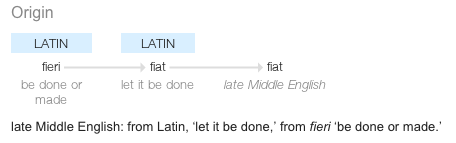
\includegraphics[width=8cm]{assets/images/fiat-definition.png}
  \caption{fiat --- 'Let it be done'}
  \label{fig:fiat-definition}
\end{figure}

Until recently, two types of money were used: \textbf{commodity money}, made
out of precious \textit{things}, and \textbf{representative money}, which simply
\textit{represents} the precious thing, mostly in writing.

We already touched on commodity money above. People used special bones,
seashells, and precious metals as money. Later on, mainly coins made out of
precious metals like gold and silver were used as money. The oldest coin found
so far is made of a natural gold-and-silver mix and was made more than 2700
years ago.\footnote{According to the Greek historian Herodotus, writing in the
fifth century BC, the Lydians were the first people to have used gold and silver
coinage. \cite{coinage-origins}} If something is new in Bitcoin, the concept of
a coin is not it.

\begin{figure}
  \centering
  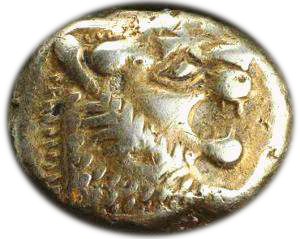
\includegraphics[width=5cm]{assets/images/lydian-coin-stater.png}
  \caption{Lydian electrum coin}
  \label{fig:lydian-coin-stater}
\end{figure}

Turns out that hoarding coins, or hodling, to use today's parlance, is
almost as old as coins. The earliest coin hodler was someone who put
almost a hundred of these coins in a pot and buried it in the
foundations of a temple, only to be found 2500 years later. Pretty good
cold storage if you ask me.

One of the downsides of using precious metal coins is that they can be
clipped, effectively debasing the value of the coin. New coins can be
minted from the clippings, inflating the money supply over time,
devaluing every individual coin in the process. People were literally
shaving off as much as they could get away with of their silver dollars.
I wonder what kind of \textit{Dollar Shave Club} advertisements they had back
in the day.

Since governments are only cool with inflation if they are the ones
doing it, efforts were made to stop this guerrilla debasement. In
classic cops-and-robbers fashion, coin clippers got ever more creative
with their techniques, forcing the 'masters of the mint' to get even
more creative with their countermeasures. Isaac Newton, the
world-renowned physicist of \textit{Principia Mathematica} fame, used to be one
of these masters. He is attributed with adding the small stripes at the
side of coins which are still present today. Gone were the days of easy
coin shaving.

\begin{figure}
  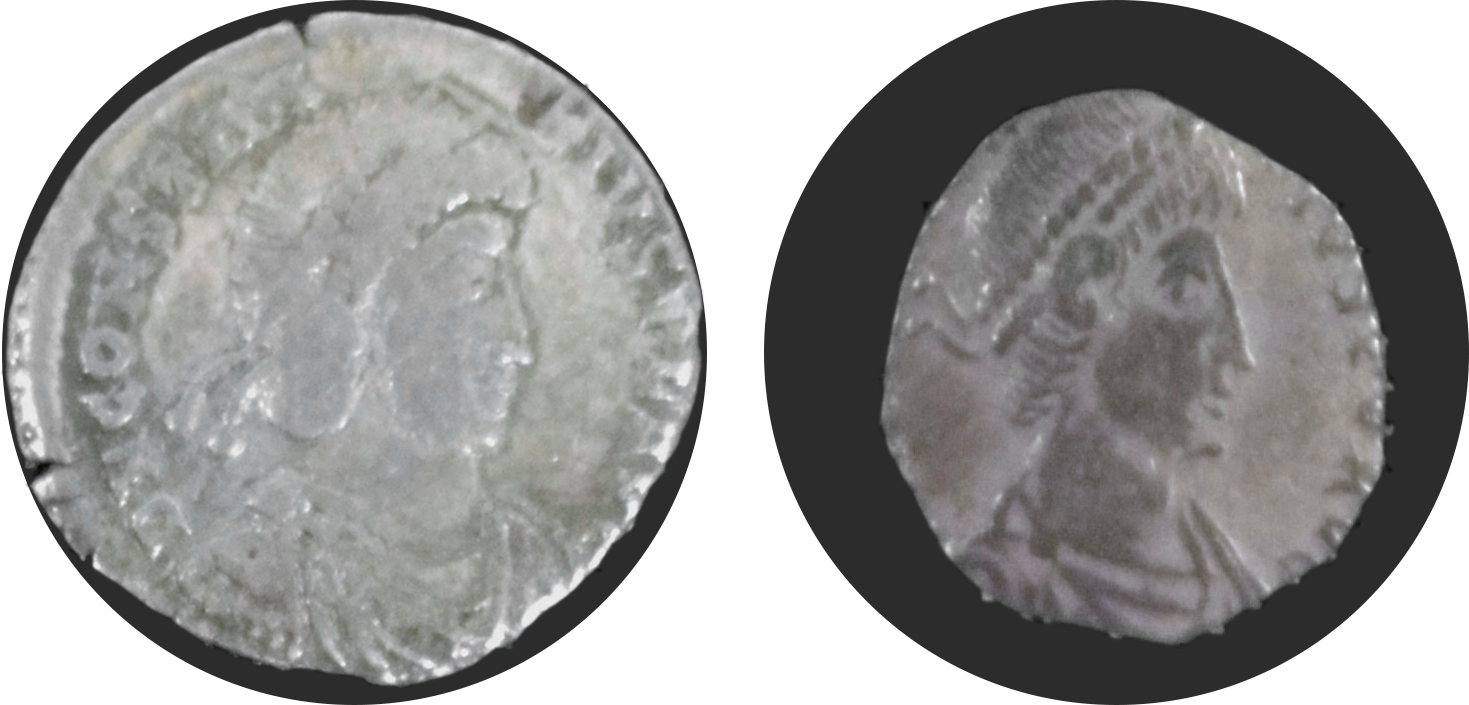
\includegraphics{assets/images/clipped-coins.png}
  \caption{Clipped silver coins of varying severity.}
  \label{fig:clipped-coins}
\end{figure}

Even with these methods of coin debasement\footnote{Besides clipping, sweating
(shaking the coins in a bag and collecting the dust worn off) and plugging
(punching a hole in the middle and hammering the coin flat to close the hole)
were the most prominent methods of coin debasement. \cite{wiki:coin-debasement}}
kept in check, coins still suffer from other issues. They are bulky and not very
convenient to transport, especially when large transfers of value need to
happen. Showing up with a huge bag of silver dollars every time you want to buy
a Mercedes isn't very practical.

Speaking of German things: How the United States \textit{dollar} got its name is
another interesting story. The word \enquote{dollar} is derived from the German word
\textit{Thaler}, short for a \textit{Joachimsthaler}~\cite{wiki:thaler}. A
Joachimsthaler was a coin minted in the town of \textit{Sankt Joachimsthal}.
Thaler is simply a shorthand for someone (or something) coming from the valley,
and because Joachimsthal was \textit{the} valley for silver coin production,
people simply referred to these silver coins as \textit{Thaler.} Thaler (German)
morphed into daalders (Dutch), and finally dollars (English).

\begin{figure}
  \centering
  
\includegraphics[width=5cm]{assets/images/joachimsthaler.png}
  \caption{The original `dollar'. Saint Joachim is pictured with his robe and wizard hat. Picture cc-by-sa Wikipedia user Berlin-George}
  \label{fig:joachimsthaler}
\end{figure}

The introduction of representative money heralded the downfall of hard
money. Gold certificates were introduced in 1863, and about fifteen
years later, the silver dollar was also slowly but surely being replaced
by a paper proxy: the silver certificate. \cite{wiki:silver-certificate}

It took about 50 years from the introduction of the first silver
certificates until these pieces of paper morphed into something that we
would today recognize as one U.S. dollar.

\begin{figure}
  \centering
  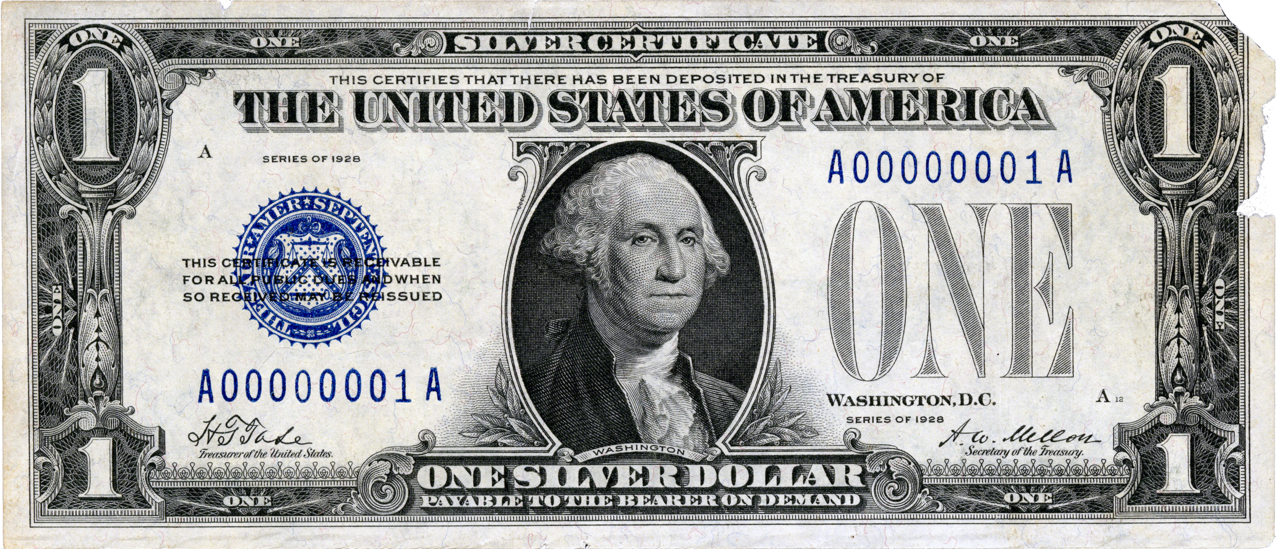
\includegraphics{assets/images/us-silver-dollar-note-smaller.png}
  \caption{A 1928 U.S. silver dollar. `Payable to the bearer on demand.' Picture credit to the National Numismatic Collection at the Smithsonian Institution}
  \label{fig:us-silver-dollar-note-smaller}
\end{figure}

Note that the 1928 U.S. silver dollar above still goes by the name of
\textit{silver certificate}, indicating that this is indeed simply a document
stating that the bearer of this piece of paper is owed a piece of
silver. It is interesting to see that the text which indicates this got
smaller over time. The trace of \enquote{certificate} vanished completely after
a while, being replaced by the reassuring statement that these are
federal reserve notes.

As mentioned above, the same thing happened to gold. Most of the world was on a
bimetallic standard~\cite{wiki:bimetallism}, meaning coins were made
primarily of gold and silver. Having certificates for gold, redeemable in gold
coins, was arguably a technological improvement. Paper is more convenient,
lighter, and since it can be divided arbitrarily by simply printing a smaller
number on it, it is easier to break into smaller units.

To remind the bearers (users) that these certificates were
representative for actual gold and silver, they were colored accordingly
and stated this clearly on the certificate itself. You can fluently read
the writing from top to bottom:

\begin{samepage}\begin{quotation}
\enquote{This certifies that there have been deposited in the treasury of the
United States of America one hundred dollars in gold coin payable to
the bearer on demand.}
\end{quotation}\end{samepage}

\begin{figure}
  \centering
  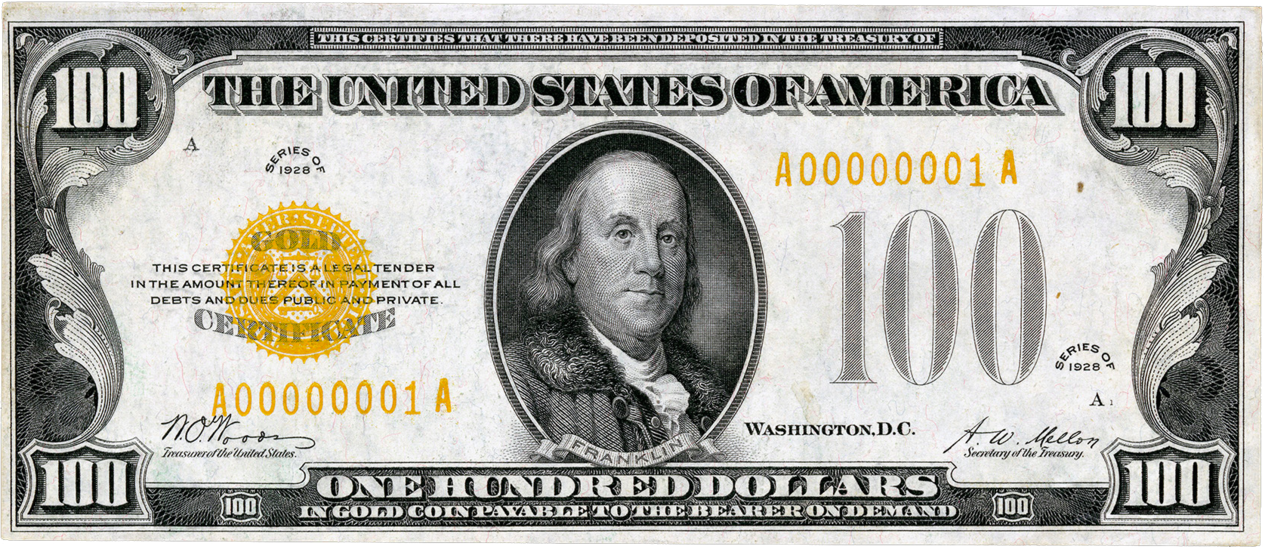
\includegraphics{assets/images/us-gold-cert-100-smaller.png}
  \caption{Picture credit to National Numismatic Collection, National Museum of American History.}
  \label{fig:us-gold-cert-100-smaller}
\end{figure}

In 1963, the words \enquote{PAYABLE TO THE BEARER ON DEMAND} were removed from
all newly issued notes. Five years later, the redemption of paper notes
for gold and silver ended.

The words hinting on the origins and the idea behind paper money were
removed. The golden color disappeared. All that was left was the paper
and with it the ability of the government to print as much of it as it
wishes.

With the abolishment of the gold standard in 1971, this century-long
sleight-of-hand was complete. Money became the illusion we all share to
this day: fiat money. It is worth something because someone commanding
an army and operating jails says it is worth something. As can be
clearly read on every dollar note in circulation today, \enquote{THIS NOTE IS
LEGAL TENDER}. In other words: It is valuable because the note says so.

\begin{figure}
  \centering
  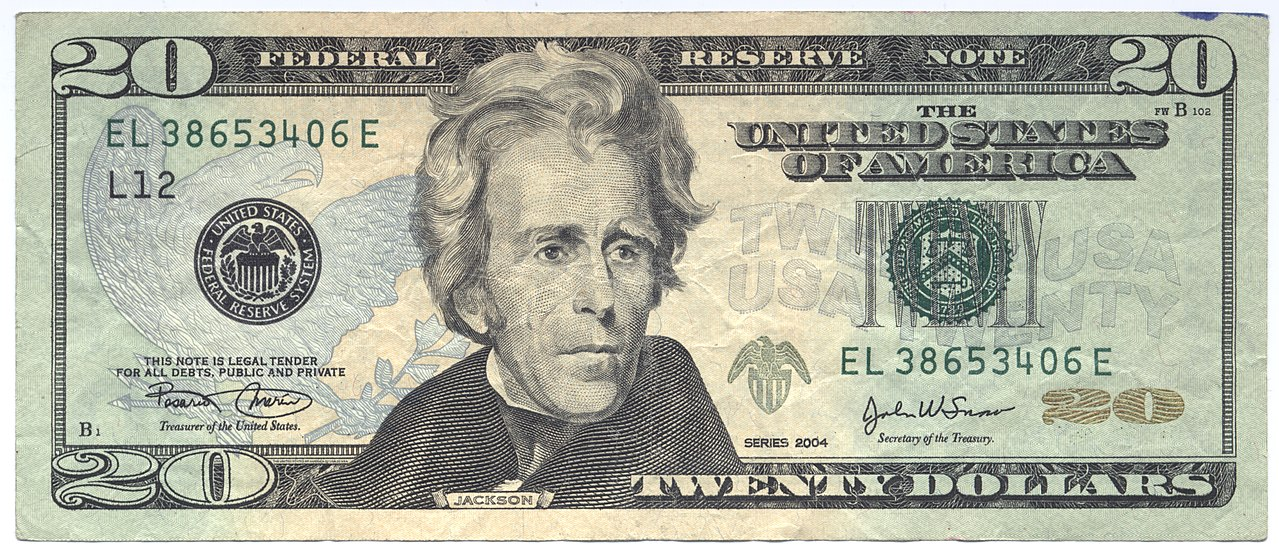
\includegraphics{assets/images/us-dollar-2004.jpg}
  \caption{A 2004 series U.S. twenty dollar note used today. `THIS NOTE IS LEGAL TENDER'}
  \label{fig:us-dollar-2004}
\end{figure}

By the way, there is another interesting lesson on today's bank notes,
hidden in plain sight. The second line reads that this is legal tender
\enquote{FOR ALL DEBTS, PUBLIC AND PRIVATE}. What might be obvious to economists
was surprising to me: All money is debt. My head is still hurting
because of it, and I will leave the exploration of the relation of money
and debt as an exercise to the reader.

As we have seen, gold and silver were used as money for millennia. Over
time, coins made from gold and silver were replaced by paper. Paper
slowly became accepted as payment. This acceptance created an
illusion --- the illusion that the paper itself has value. The final
move was to completely sever the link between the representation and the
actual: abolishing the gold standard and convincing everyone that the
paper in itself is precious.

\paragraph{Bitcoin taught me about the history of money and the greatest sleight of
hand in the history of economics: fiat currency.}

% ---
%
% #### Down the Rabbit Hole
%
% - [Shelling Out: The Origins of Money] by Nick Szabo
% - [Methods of Coin Debasement][coin debasement], [Thaler], [U.S. Silver Certificate][silver certificates], [Bimetallism][bimetallic standard] on Wikipedia
%
% [oldest coin]: https://www.britishmuseum.org/explore/themes/money/the_origins_of_coinage.aspx
% [coin debasement]: https://en.wikipedia.org/wiki/Methods_of_coin_debasement
% [Thaler]: https://en.wikipedia.org/wiki/Thaler
% [Berlin-George]: https://en.wikipedia.org/wiki/File:Bohemia,_Joachimsthaler_1525_Electrotype_Copy._VF._Obverse..jpg
% [silver certificates]: https://en.wikipedia.org/wiki/Silver_certificate_%28United_States%29
% [bimetallic standard]: https://en.wikipedia.org/wiki/Bimetallism
% [Shelling Out: The Origins of Money]: https://nakamotoinstitute.org/shelling-out/
%
% <!-- Wikipedia -->
% [alice]: https://en.wikipedia.org/wiki/Alice%27s_Adventures_in_Wonderland
% [carroll]: https://en.wikipedia.org/wiki/Lewis_Carroll

\chapter{Fractional Reserve Insanity}
\label{les:13}

\begin{chapquote}{Lewis Carroll, \textit{Alice in Wonderland}}
Alas! it was too late: she went on growing and growing, and very soon had to
kneel down: in another minute there was not room even for this, and she tried
the effect of lying down, with one elbow against the door, and the other arm
curled round her head. Still she went on growing, and as a last resource she put
one arm out of the window, and one foot up the chimney, and said to herself
``now I can do no more—what will become of me?''
\end{chapquote}

Value and money aren't trivial topics, especially in today's times. The
process of money creation in our banking system is equally non-trivial,
and I can't shake the feeling that this is deliberately so. What I have
previously only encountered in academia and legal texts seems to be
common practice in the financial world as well: nothing is explained in
simple terms, not because it is truly complex, but because the truth is
hidden behind layers and layers of jargon and \textit{apparent} complexity.
"Expansionary monetary policy, quantitative easing, fiscal stimulus to
the economy." The audience nods along in agreement, hypnotized by the
fancy words.

Fractional reserve banking and quantitative easing are two of those
fancy words, obfuscating what is really happening by masking it as
complex and difficult to understand. If you would explain them to a
five-year-old, the insanity of both will become apparent quickly.

Godfrey Bloom, addressing the European Parliament during a joint
debate, said it way better than I ever could:

\begin{quotation}
[...] you do not really understand the concept of banking. All the
banks are broke. Bank Santander, Deutsche Bank, Royal Bank of
Scotland --- they're all broke! And why are they broke? It isn't an
act of God. It isn't some sort of tsunami. They're broke because we
have a system called 'fractional reserve banking' which means that
banks can lend money that they don't actually have! It's a criminal
scandal and it's been going on for too long. [...]
We have counterfeiting --- sometimes called quantitative
easing --- but counterfeiting by any other name. The artificial
printing of money which, if any ordinary person did, they'd go to
prison for a very long time [...] and until we start sending
bankers --- and I include central bankers and politicians --- to
prison for this outrage it will continue.
\flushright -- Godfrey Bloom\footnote{Joint debate on the
banking union~\cite{godfrey-bloom}}
\end{quotation}

Let me repeat the most important part: banks can lend money that they
don't actually have.

Thanks to fractional reserve banking, a bank only has to keep a small
\textit{fraction} of every dollar it gets. It's somewhere between 0 and 10%,
usually at the lower end, which makes things even worse.

Let's use a concrete example to better understand this crazy idea: A
fraction of 10\% will do the trick and we should be able to do all the
calculations in our head. Win-win. So, if you take \$100 to a
bank --- because you don't want to store it under your mattress --- they
only have to keep the agreed upon \textit{fraction} of it. In our example that
would be \$10, because 10\% of \$100 is \$10. Easy, right?

So what do banks do with the rest of the money? What happens to your \$90? They
do what banks do, they lend it to other people. The result is a money multiplier
effect, which increases the money supply in the economy enormously
(Figure~\ref{fig:money-multiplier}). Your initial deposit of \$100 will soon
turn into \$190. By lending a 90\% fraction of the newly created \$90, there
will soon be \$271 in the economy \cite{wiki:money-multiplier}. And \$343.90 after that. The money supply is
recursively increasing, since banks are literally lending money they don't have.
Without a single Abracadabra, banks magically transform \$100 into one thousand
dollars or more. Turns out 10x is easy. It only takes a couple of lending
rounds.

\begin{figure}
  \centering
  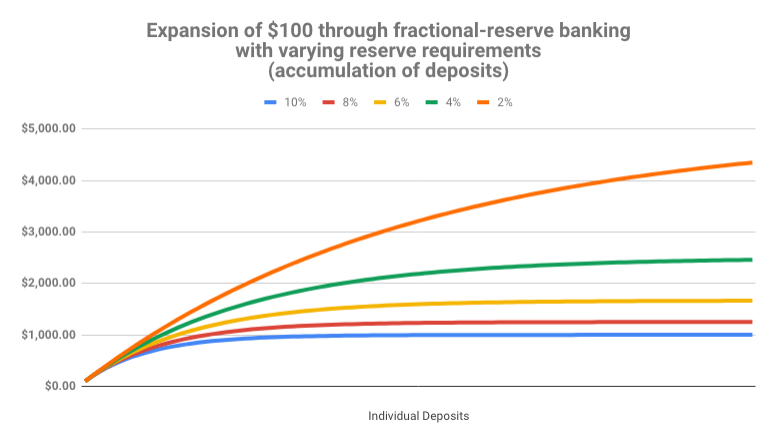
\includegraphics{assets/images/money-multiplier.png}
  \caption{The money multiplier effect}
  \label{fig:money-multiplier}
\end{figure}

Don't get me wrong: There is nothing wrong with lending. There is
nothing wrong with interest. There isn't even anything wrong with good
old regular banks to store your wealth somewhere more secure than in
your sock drawer.

Central banks, however, are a different beast. Abominations of financial
regulation, half public half private, playing god with something which
affects everyone who is part of our global civilization, without a
conscience, only interested in the immediate future, and seemingly
without any accountability or auditability (see Figure~\ref{fig:bsg}).

\begin{figure}
  \centering
  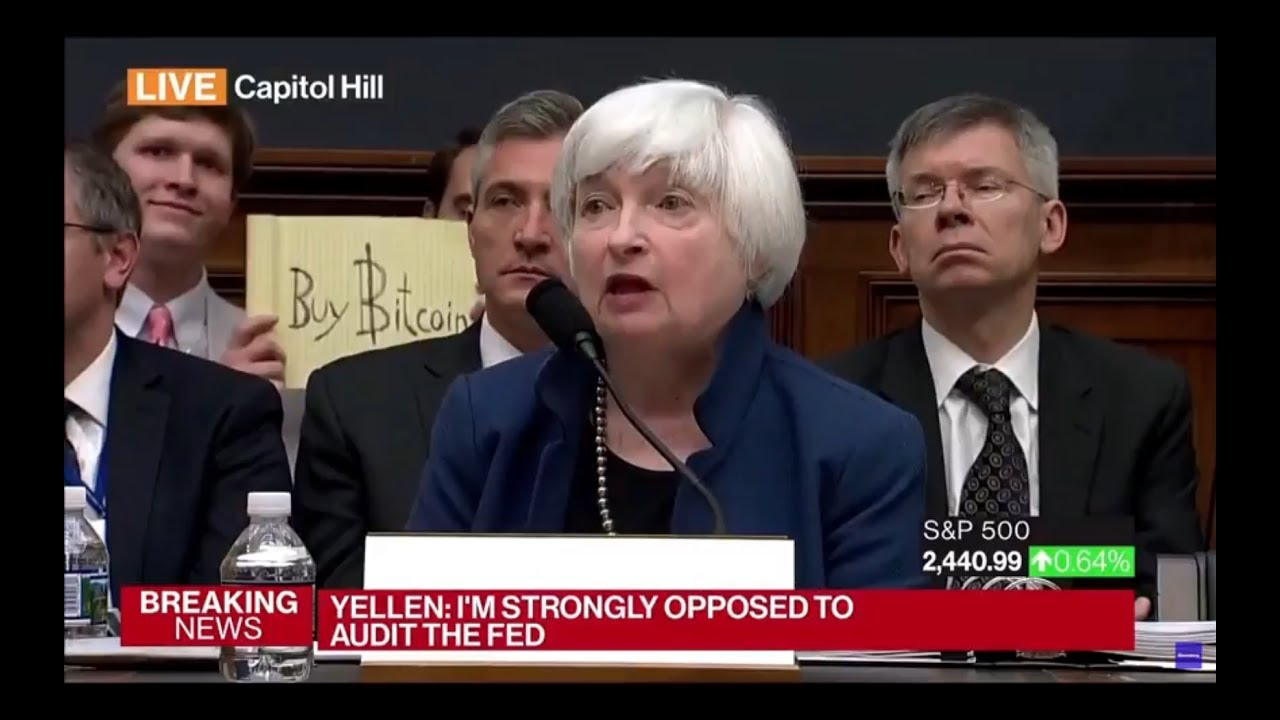
\includegraphics{assets/images/bsg.jpg}
  \caption{Yellen is strongly opposed to audit the fed, while BSG is strongly in favor to buy bitcoin.}
  \label{fig:bsg}
\end{figure}

While Bitcoin is still inflationary, it will cease to be so rather soon.
The strictly limited supply of 21 million bitcoins will eventually do
away with inflation completely. We now have two monetary worlds: an
inflationary one where money is printed arbitrarily, and the world of
Bitcoin, where final supply is fixed and easily auditable for everyone.
One is forced upon us by violence, the other can be joined by anyone who
wishes to do so. No barriers to entry, no one to ask for permission.
Voluntary participation. That is the beauty of Bitcoin.

I would argue that the argument between Keynesian\footnote{Theories according to
John Maynard Keynes and his deciples~\cite{wiki:keynesian}} and
Austrian\footnote{School of economic thought based on methodological
individualism~\cite{wiki:austrian}} economists is no longer purely academical.
Satoshi managed to build a system for value transfer on steroids, creating the
soundest money which ever existed in the process. One way or another, more and
more people will learn about the scam which is fractional reserve banking. If
they come to similar conclusions as most Austrians and Bitcoiners, they might
join the ever-growing internet of money. Nobody can stop them if they choose to
do so.

\paragraph{Bitcoin taught me that fractional reserve banking is pure insanity.}

% ---
%
% #### Down the Rabbit Hole
%
% - [The Creature From Jekyll Island] by G. Edward Griffin
% - [Money Multiplier][money multiplier], [Keynesian Economics][Keynesian], [Austrian School][Austrian] on Wikipedia
%
% [The Creature From Jekyll Island]: https://archive.org/details/pdfy--Pori1NL6fKm2SnY
%
% [joint debate]: https://www.youtube.com/watch?v=hYzX3YZoMrs
% [money multiplier]: https://en.wikipedia.org/wiki/Money_multiplier
% [auditability]: https://i.ytimg.com/vi/ThFGs347MW8/maxresdefault.jpg
% [Keynesian]: https://en.wikipedia.org/wiki/Keynesian_economics
% [Austrian]: https://en.wikipedia.org/wiki/Austrian_School
%
% <!-- Wikipedia -->
% [alice]: https://en.wikipedia.org/wiki/Alice%27s_Adventures_in_Wonderland
% [carroll]: https://en.wikipedia.org/wiki/Lewis_Carroll

\chapter{ Sound Money}
\label{les:14}

\begin{chapquote}{Lewis Carroll, \textit{Alice in Wonderland}}
``The first thing I've got to do,'' said Alice to herself, as she wandered about
in the wood, ``is to grow to my right size, and the second thing is to find my
way into that lovely garden. I think that will be the best plan.''
\end{chapquote}

The most important lesson I have learned from Bitcoin is that in the
long run, hard money is superior to soft money. Hard money, also
referred to as *sound money*, is any globally traded currency that
serves as a reliable store of value.

Granted, Bitcoin is still young and volatile. Critics will say that it
does not store value reliably. The volatility argument is missing the
point. Volatility is to be expected. The market will take a while to
figure out the just price of this new money. Also, as is often jokingly
pointed out, it is grounded in an error of measurement. If you think in
dollars you will fail to see that one bitcoin will always be worth one
bitcoin.

\begin{quotation}
``A fixed money supply, or a supply altered only in accord with
objective and calculable criteria, is a necessary condition to a
meaningful just price of money.''
\end{quotation}
% > <cite>[Fr. Bernard W. Dempsey, S.J.]</cite>

As a quick stroll through the graveyard of forgotten currencies has
shown, money which can be printed will be printed. So far, no human in
history was able to resist this temptation.

Bitcoin does away with the temptation to print money in an ingenious
way. Satoshi was aware of our greed and fallibility --- this is why he
chose something more reliable than human restraint: mathematics.

\begin{figure}
  \centering
  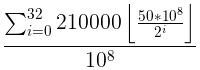
\includegraphics{assets/images/supply-formula-white.png}
  \caption{Bitcoin's supply formula}
  \label{fig:supply-formula-white}
\end{figure}

\begin{equation}
\sum\limits_{i=0}^{32} \frac{21000}{10^8}
\end{equation}

% 

While this formula is useful to describe Bitcoin's supply, it is
actually nowhere to be found in the code. Issuance of new bitcoin is
done in an [algorithmically controlled] fashion, by reducing the reward
which is paid to miners every four years. The formula above is used to
quickly sum up what is happening under the hood. What really happens can
be best seen by looking at the change in block reward, the reward paid
out to whoever finds a valid block, which roughly happens every 10
minutes.

% 

Formulas, logarithmic functions and exponentials are not exactly
intuitive to understand. The concept of *soundness* might be easier to
understand if looked at in another way. Once we know how much there is
of something, and once we know how hard this something is to produce or
get our hands on, we immediately understand its value. What is true for
Picasso's paintings, Elvis Presley's guitars, and Stradivarius violins
is also true for fiat currency, gold, and bitcoins.

The hardness of fiat currency depends on who is in charge of the
respective printing presses. Some governments might be more willing to
print large amounts of currency than others, resulting in a weaker
currency. Other governments might be more restrictive in their money
printing, resulting in harder currency.

Before we had fiat currencies, the soundness of money was determined by
the natural properties of the stuff which we used as money. The amount
of gold on earth is limited by the laws of physics. Gold is rare because
supernovae and neutron star collisions are rare. The "flow" of gold is
limited because extracting it is quite an effort. Being a heavy element
it is mostly buried deep underground.

The abolishment of the gold standard gave way to a new reality: adding
new money requires just a drop of ink. In our modern world adding a
couple of zeros to the balance of a bank account requires even less
effort: flipping a few bits in a bank computer is enough.

\begin{quotation}
``One important aspect of this new reality is that institutions like
the Fed cannot go bankrupt. They can print any amount of money that
they might need for themselves at virtually zero cost.''
\end{quotation}
% <cite>[Jörg Guido Hülsmann]</cite>

The principle outlined above can be expressed more generally as the
ratio of "stock" to "flow". Simply put, the *stock* is how much of
something is currently there. For our purposes, the stock is a measure
of the current money supply. The *flow* is how much there is produced
over a period of time (e.g. per year). The key to understanding sound
money is in understanding this stock-to-flow ratio.

Calculating the stock-to-flow ratio for fiat currency is difficult,
because [how much money there is] depends on how you look at it. You
could count only banknotes and coins (M0), add traveler checks and check
deposits (M1), add saving accounts and mutual funds and some other
things (M2), and even add certificates of deposit to all of that (M3).
Further, how all of this is defined and measured varies from country to
country and since the US Federal Reserve [stopped publishing] numbers
for M3, we will have to make do with the M2 monetary supply. I would
love to verify these numbers, but I guess we have to trust the fed for
now.

Gold, one of the rarest metals on earth, has the highest stock-to-flow
ratio. According to the US Geological Survey, a little more than 190,000
tons have been mined. In the [last few years], around 3100 tons of gold
have been mined per year.

Using these numbers, we can easily calculate the stock-to-flow ratio for
gold: 190,000 tons / 3,100 tons = \~61.

Nothing has a higher stock-to-flow ratio than gold. This is why gold, up
to now, was the hardest, soundest money in existence. It is often said
that all the gold mined so far would fit in two olympic-sized swimming
pools. According to [my calculations], we would need four. So maybe this
needs updating, or Olympic-sized swimming pools got smaller.

Enter Bitcoin. As you probably know, bitcoin mining was all the rage in
the last couple of years. This is because we are still in the early
phases of what is called the *reward era*, where mining nodes are
rewarded with *a lot* of bitcoin for their computational effort. We are
currently in reward era number 3, which began in 2016 and will end in
early 2020, probably in May. While the bitcoin supply is predetermined,
the inner workings of Bitcoin only allow for approximate dates.
Nevertheless, we can predict with certainty how high Bitcoin's
stock-to-flow ratio will be. Spoiler alert: it will be high.

How high? Well, it turns out that Bitcoin will get infinitely hard.

% 



Due to an exponential decrease of the mining reward, the flow of new
bitcoin will diminish resulting in a sky-rocketing stock-to-flow ratio.
It will catch up to gold in 2020, only to surpass it four years later by
doubling its soundness again. Such a doubling will occur 64 times in
total. Thanks to the power of exponentials, the number of bitcoin mined
per year will drop below 100 bitcoin in 50 years and below 1 bitcoin in
75 years. The global faucet which is the block reward will dry up
somewhere around the year 2140, effectively stopping the production of
bitcoin. This is a long game. If you are reading this, you are still
early.

% 

As bitcoin approaches infinite stock to flow ratio it will be the
soundest money in existence. Infinite soundness is hard to beat.

Viewed through the lens of economics, Bitcoin's *difficulty adjustment*
is probably its most important component. How hard it is to mine bitcoin
depends on how quickly new bitcoins are mined\*. It is the dynamic
adjustment of the network's mining difficulty which enables us to
predict its future supply.

*(\* It actually depends on how quickly valid blocks are found, but for
our purposes, this is the same thing as "mining bitcoins" and will be so
for the next 120 years.)*

The simplicity of the difficulty adjustment algorithm might distract
from its profundity, but the difficulty adjustment truly is a revolution
of Einsteinian proportions. It ensures that, no matter how much or how
little effort is spent on mining, Bitcoin's controlled supply won't be
disrupted. As opposed to every other resource, no matter how [much
energy] someone will put into mining bitcoin, the total reward will not
increase.

Just like $E=mc^2$ dictates the [universal speed limit] in our universe,
Bitcoin's difficulty adjustment dictates the **universal money limit**
in Bitcoin.

If it weren't for this difficulty adjustment, all bitcoins would have
been mined already. If it weren't for this difficulty adjustment,
Bitcoin probably wouldn't have survived in its infancy. It is what
secures the network in its reward era. It is what ensures a steady and
[fair distribution] of new bitcoin. It is the thermostat which regulates
Bitcoin's monetary policy.

Einstein showed us something novel: no matter how hard you push an
object, at a certain point you won't be able to get more speed out of
it. Satoshi also showed us something novel: no matter how hard you dig
for this digital gold, at a certain point you won't be able to get more
bitcoin out of it. For the first time in human history, we have a
monetary good which, no matter how hard you try, you won't be able to
produce more of.

Bitcoin taught me that sound money is essential.

% ---
%
% #### Through the Looking-Glass
%
% - [Bitcoin's Energy Consumption: A Shift in Perspective][much energy]
%
% #### Down the Rabbit Hole
%
% - [The Ethics of Money Production][Jörg Guido Hülsmann] by Jörg Guido Hülsmann
% - [Mineral Commodity Summaries 2019][last few years] by the United States Geological Survey
% - [Bitcoin’s Distribution was Fair][fair distribution] by Dan Held
% - [Bitcoin's Controlled Supply][algorithmically controlled] on the Bitcoin Wiki
% - [Money Supply][how much money there is], [Speed of Light][universal speed limit] on Wikipedia
%
% <!-- Internal -->
% [much energy]: 
%
% [Fr. Bernard W. Dempsey, S.J.]: https://www.jstor.org/stable/29769582
% [Jörg Guido Hülsmann]: https://mises.org/sites/default/files/The%20Ethics%20of%20Money%20Production_2.pdf
% [stopped publishing]: https://www.federalreserve.gov/Releases/h6/discm3.htm
% [last few years]: https://minerals.usgs.gov/minerals/pubs/mcs/2018/mcs2018.pdf
% [my calculations]: https://www.wolframalpha.com/input/?i=volume+of+190000+metric+tons+gold+%2F+olympic+swimming+pool+volume
% [fair distribution]: https://blog.picks.co/bitcoins-distribution-was-fair-e2ef7bbbc892
%
% <!-- Bitcoin Wiki -->
% [algorithmically controlled]: https://en.bitcoin.it/wiki/Controlled_supply
%
% <!-- Wikipedia -->
% [how much money there is]: https://en.wikipedia.org/wiki/Money_supply
% [universal speed limit]: https://en.wikipedia.org/wiki/Speed_of_light#Upper_limit_on_speeds
% [alice]: https://en.wikipedia.org/wiki/Alice%27s_Adventures_in_Wonderland
% [carroll]: https://en.wikipedia.org/wiki/Lewis_Carroll

\part{Technology}
\label{ch:technology}

\begin{chapquote}{Lewis Carroll, \textit{Alice in Wonderland}}
``Now, I'll manage better this time'' she said to herself, and began by taking
the little golden key, and unlocking the door that led into the garden
\end{chapquote}

\newthought{Golden keys}, clocks which only work by chance, races to solve
strange riddles, and builders that don't have faces or names. What sounds like
fairy tales from Wonderland is daily business in the world of Bitcoin.

As we explored in [Chapter 2][chapter2], large parts of the current financial
system are systematically broken. Like Alice, we can only hope to manage better
this time. But, thanks to a pseudonymous inventor, we have incredibly
sophisticated technology to support us this time around: Bitcoin.

Solving problems in a radically decentralized and adversarial environment
requires unique solutions. What would otherwise be trivial problems to solve
are everything but in this strange world of nodes. Bitcoin relies on strong
cryptography for most solutions, at least if looked at through the lens of
technology. Just how strong this cryptography is will be explored in one of the
following lessons.

\newthought{Cryptography} is what Bitcoin uses to remove trust in authorities.
Instead of relying on centralized institutions, the system relies on the final
authority of our universe: physics. Some grains of trust still remain, however.
We will examine these grains in the second lesson of this chapter.

% 

The last couple of lessons explore the ethos of technological development in
Bitcoin, which is arguably as important as the technology itself. Bitcoin is not
the next shiny app on your phone. It is the foundation of a new economic
reality, which is why Bitcoin should be treated as nuclear-grade financial
software.

Where are we in this financial, societal, and technological revolution? Networks
and technologies of the past may serve as metaphors for Bitcoins future, which
are explored in the last lesson of this chapter.

Once more, strap in and enjoy the ride. Like all exponential technologies, we
are about to go parabolic.

\chapter{Strength in Numbers}
\label{les:15}

\begin{chapquote}{Lewis Carroll, \textit{Alice in Wonderland}}
\enquote{Let me see: four times five is twelve, and four times six is thirteen, and
four times seven is fourteen—oh dear! I shall never get to twenty at this
rate!}
\end{chapquote}

Numbers are an essential part of our everyday life. Large numbers,
however, aren't something most of us are too familiar with. The largest
numbers we might encounter in everyday life are in the range of
millions, billions, or trillions. We might read about millions of people
in poverty, billions of dollars spent on bank bailouts, and trillions of
national debt. Even though it's hard to make sense of these headlines,
we are somewhat comfortable with the size of those numbers.

Although we might seem comfortable with billions and trillions, our
intuition already starts to fail with numbers of this magnitude. Do you
have an intuition how long you would have to wait for a
million/billion/trillion seconds to pass? If you are anything like me,
you are lost without actually crunching the numbers.

Let's take a closer look at this example: the difference between each is an
increase by three orders of magnitude: $10^6$, $10^9$, $10^{12}$. Thinking about
seconds is not very useful, so let's translate this into something we can wrap
our head around:

\begin{itemize}
  \item $10^6$: One million seconds was $1 1/2$ weeks ago.
  \item $10^9$: One billion seconds was almost 32 years ago.
  \item $10^{12}$: One trillion seconds ago Manhattan was covered under a thick
  layer of ice.\footnote{One trillion seconds ($10^{12}$) was $31710$ years ago. The Last Glacial
  Maximum was $33,000$ years ago.~\cite{wiki:LGM}}
\end{itemize}

\begin{figure}
  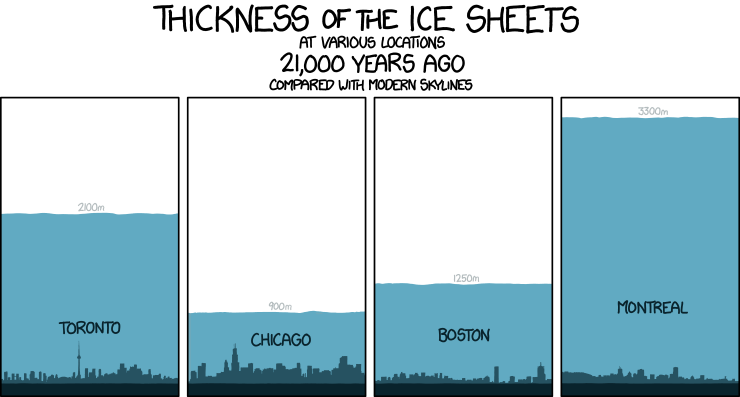
\includegraphics{assets/images/xkcd-1225.png}
  \caption{About 1 trillion seconds ago. Source: xkcd 1225}
  \label{fig:xkcd-1225}
\end{figure}

As soon as we enter the beyond-astronomical realm of modern
cryptography, our intuition fails catastrophically. Bitcoin is built
around large numbers and the virtual impossibility of guessing them.
These numbers are way, way larger than anything we might encounter in
day-to-day life. Many orders of magnitude larger. Understanding how
large these numbers truly are is essential to understanding Bitcoin as a
whole.

Let's take SHA-256\footnote{SHA-256 is part of the SHA-2 family of cryptographic
hash functions developed by the NSA.~\cite{wiki:sha2}}, one of the hash
functions\footnote{Bitcoin uses SHA-256 in its block hashing
algorithm.~\cite{btcwiki:block-hashing}} used in Bitcoin, as a concrete example.
It is only natural to think about 256 bits as \enquote{two hundred fifty-six,} which
isn't a large number at all. However, the number in SHA-256 is talking about
orders of magnitude --- something our brains are not well-equipped to deal with.

While bit length is a convenient metric, the true meaning of 256-bit
security is lost in translation. Similar to the millions ($10^6$) and
billions ($10^9$) above, the number in SHA-256 is about orders of magnitude
($2^{256}$).

So, how strong is SHA-256, exactly?

\begin{quotation}\begin{samepage}
\enquote{SHA-256 is very strong. It's not like the incremental step from MD5
to SHA1. It can last several decades unless there's some massive
breakthrough attack.}
\begin{flushright} -- Satoshi Nakamoto\footnote{Satoshi Nakamoto, in a reply to questions about SHA-256 collisions. \cite{satoshi-sha256}}
\end{flushright}\end{samepage}\end{quotation}

Let's spell things out. $2^{256}$ equals the following number:

\begin{quotation}\begin{samepage}
    115 quattuorvigintillion 792 trevigintillion 89 duovigintillion 237
    unvigintillion 316 vigintillion 195 novemdecillion 423 octodecillion 570
    septendecillion 985 sexdecillion 8 quindecillion 687 quattuordecillion 907
    tredecillion 853 duodecillion 269 undecillion 984 decillion 665 nonillion
    640 octillion 564 septillion 39 sextillion 457 quintillion 584 quadrillion 7
    trillion 913 billion 129 million 639 thousand 936.
\end{samepage}\end{quotation}

That's a lot of nonillions! Wrapping your head around this number is
pretty much impossible. There is nothing in the physical universe to
compare it to. It is far larger than the number of atoms in the
observable universe. The human brain simply isn't made to make sense of
it.

\newpage

One of the best visualizations of the true strength of SHA-256 is a video by
Grant Sanderson. Aptly named \textit{\enquote{How secure is 256 bit
security?}}\footnote{Watch the video at \url{https://youtu.be/S9JGmA5_unY}} it
beautifully shows how large a 256-bit space is. Do yourself a favor and take the
five minutes to watch it. As all other \textit{3Blue1Brown} videos it is not
only fascinating but also exceptionally well made. Warning: You might fall down
a math rabbit hole.

\begin{figure}
  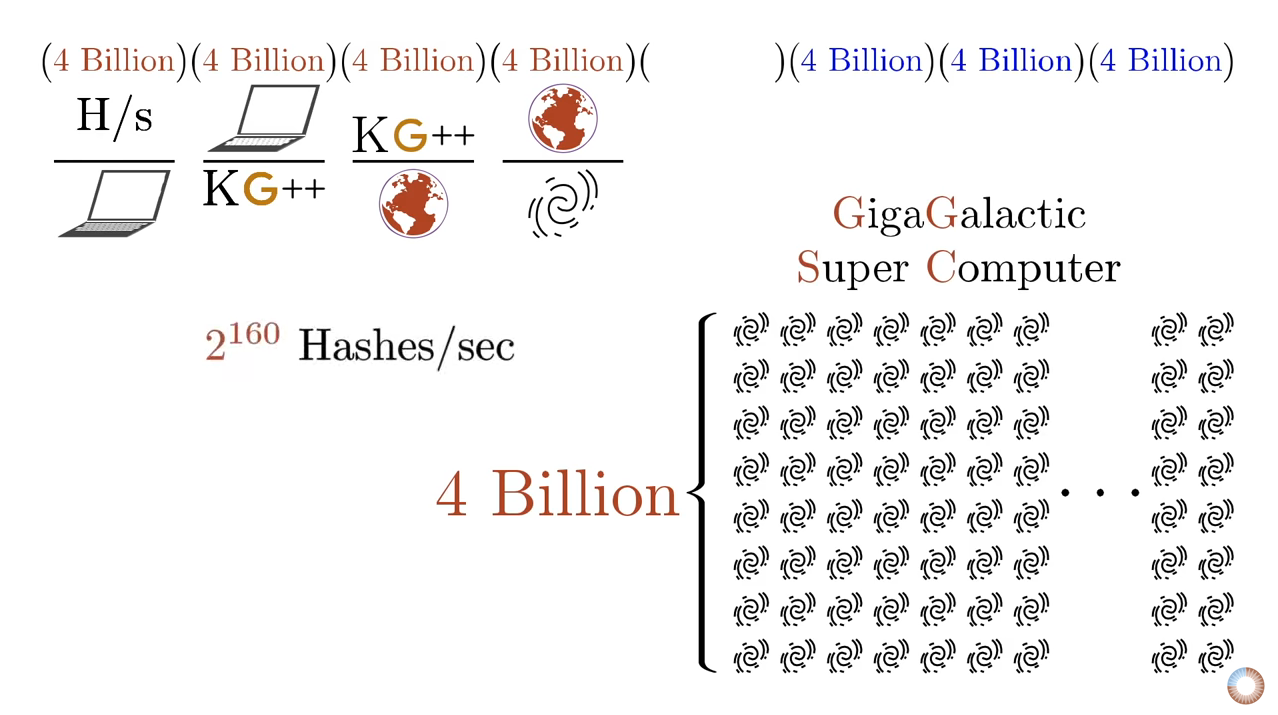
\includegraphics{assets/images/youtube-vid-inverted.png}
  \caption{Illustration of SHA-256 security. Original graphic by Grant Sanderson aka 3Blue1Brown.}
  \label{fig:youtube-vid-inverted}
\end{figure}

Bruce Schneier~\cite{web:schneier} used the physical limits of computation to put this
number into perspective: even if we could build an optimal computer,
which would use any provided energy to flip bits perfectly~\cite{wiki:landauer}, build a
Dyson sphere\footnote{A Dyson sphere is a hypothetical megastructure that completely encompasses a star and captures a large percentage of its power output.~\cite{wiki:dyson}} around our sun, and let it run for 100 billion billion
years, we would still only have a $25\%$ chance to find a needle in a
256-bit haystack.

\begin{quotation}\begin{samepage}
\enquote{These numbers have nothing to do with the technology of the devices;
they are the maximums that thermodynamics will allow. And they
strongly imply that brute-force attacks against 256-bit keys will be
infeasible until computers are built from something other than matter
and occupy something other than space.}
\begin{flushright} -- Bruce Schneier\footnote{Bruce Schneier, \textit{Applied Cryptography} \cite{bruce-schneier}}
\end{flushright}\end{samepage}\end{quotation}


It is hard to overstate the profoundness of this. Strong cryptography
inverts the power-balance of the physical world we are so used to.
Unbreakable things do not exist in the real world. Apply enough force,
and you will be able to open any door, box, or treasure chest.

Bitcoin's treasure chest is very different. It is secured by strong
cryptography, which does not give way to brute force. And as long as the
underlying mathematical assumptions hold, brute force is all we have.
Granted, there is also the option of a global \$5 wrench attack (Figure~\ref{fig:xkcd-538})
But torture won't work for all bitcoin addresses, and the cryptographic
walls of bitcoin will defeat brute force attacks. Even if you come at it
with the force of a thousand suns. Literally.

\begin{figure}
  \centering
  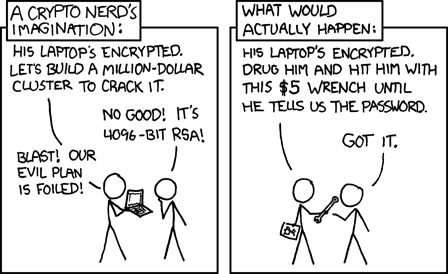
\includegraphics[width=8cm]{assets/images/xkcd-538.png}
  \caption{\$5 wrench attack. Source: xkcd 538}
  \label{fig:xkcd-538}
\end{figure}

This fact and its implications were poignantly summarized in the call
to cryptographic arms: \textit{\enquote{No amount of coercive force will ever solve
a math problem.}}

\begin{quotation}\begin{samepage}
\enquote{It isn't obvious that the world had to work this way. But somehow the
universe smiles on encryption.}
\begin{flushright} -- Julian Assange\footnote{Julian Assange, \textit{A Call to Cryptographic Arms} \cite{call-to-cryptographic-arms}}
\end{flushright}\end{samepage}\end{quotation}

Nobody yet knows for sure if the universe's smile is genuine or not. It
is possible that our assumption of mathematical asymmetries is wrong and
we find that P actually equals NP \cite{wiki:pnp}, or we find surprisingly quick
solutions to specific problems \cite{wiki:discrete-log} which we currently assume to be hard.
If that should be the case, cryptography as we know it will cease to
exist, and the implications would most likely change the world beyond
recognition.

\begin{quotation}\begin{samepage}
\enquote{Vires in Numeris} = \enquote{Strength in Numbers}\footnote{\textit{Vires in Numeris} was first proposed as a Bitcoin motto by the bitcointalk user \textit{epii}~\cite{epii}}
\end{samepage}\end{quotation}

\textit{Vires in numeris} is not only a catchy motto used by bitcoiners. The
realization that there is an unfathomable strength to be found in
numbers is a profound one. Understanding this, and the inversion of
existing power balances which it enables changed my view of the world
and the future which lies ahead of us.

One direct result of this is the fact that you don't have to ask anyone
for permission to participate in Bitcoin. There is no page to sign up,
no company in charge, no government agency to send application forms to.
Simply generate a large number and you are pretty much good to go. The
central authority of account creation is mathematics. And God only knows
who is in charge of that.

\begin{figure}
  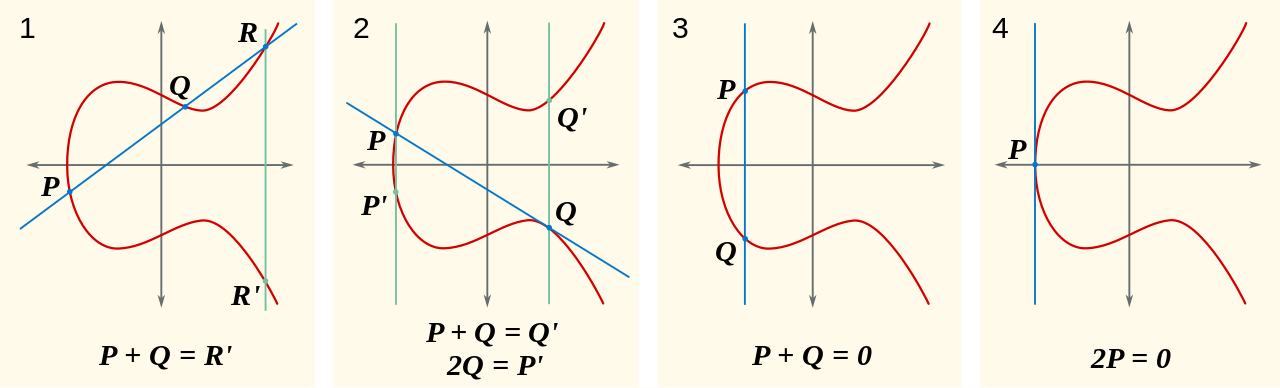
\includegraphics{assets/images/elliptic-curve-examples.png}
  \caption{Elliptic curve examples. Graphic cc-by-sa Emmanuel Boutet.}
  \label{fig:elliptic-curve-examples}
\end{figure}

Bitcoin is built upon our best understanding of reality. While there are
still many open problems in physics, computer science, and mathematics,
we are pretty sure about some things. That there is an asymmetry between
finding solutions and validating the correctness of these solutions is
one such thing. That computation needs energy is another one. In other
words: finding a needle in a haystack is harder than checking if the
pointy thing in your hand is indeed a needle or not. And finding the
needle takes work.

The vastness of Bitcoin's address space is truly mind-boggling. The
number of private keys even more so. It is fascinating how much of our
modern world boils down to the improbability of finding a needle in an
unfathomably large haystack. I am now more aware of this fact than ever.

\paragraph{Bitcoin taught me that there is strength in numbers.}

% ---
%
% #### Down the Rabbit Hole
%
% - [How secure is 256 bit security?]["How secure is 256 bit security?"] by 3Blue1Brown
% - [Block Hashing Algorithm][hash functions] on the Bitcoin Wiki
% - [Last Glacial Maximum][thick layer of ice], [SHA-2][SHA-256], [Dyson Sphere][Dyson sphere], [Landauer's Principle][flip bits perfectly] [P versus NP][P actually equals NP], [Discrete Logarithm][specific problems] on Wikipedia
%
% [thick layer of ice]: https://en.wikipedia.org/wiki/Last_Glacial_Maximum
% [xkcd \#1125]: https://xkcd.com/1225/
% [SHA-256]: https://en.wikipedia.org/wiki/SHA-2
% [hash functions]: https://en.bitcoin.it/wiki/Block_hashing_algorithm
% ["How secure is 256 bit security?"]: https://www.youtube.com/watch?v=S9JGmA5_unY
% [Bruce Schneier]: https://www.schneier.com/
% [flip bits perfectly]: https://en.wikipedia.org/wiki/Landauer%27s_principle#Equation
% [Dyson sphere]: https://en.wikipedia.org/wiki/Dyson_sphere
% [2]: https://books.google.com/books?id=Ok0nDwAAQBAJ&pg=PT316&dq=%22These+numbers+have+nothing+to+do+with+the+technology+of+the+devices;%22&hl=en&sa=X&ved=0ahUKEwjXttWl8YLhAhUphOAKHZZOCcsQ6AEIKjAA#v=onepage&q&f=false
% [wrench attack]: https://xkcd.com/538/
% [call to cryptographic arms]: https://cryptome.org/2012/12/assange-crypto-arms.htm
% [P actually equals NP]: https://en.wikipedia.org/wiki/P_versus_NP_problem#P_=_NP
% [specific problems]: https://en.wikipedia.org/wiki/Discrete_logarithm#Cryptography
% [3Blue1Brown]: https://twitter.com/3blue1brown
%
% <!-- Wikipedia -->
% [alice]: https://en.wikipedia.org/wiki/Alice%27s_Adventures_in_Wonderland
% [carroll]: https://en.wikipedia.org/wiki/Lewis_Carroll

\chapter{Reflections on ``Don't Trust, Verify''}
\label{les:16}

\begin{chapquote}{Lewis Carroll, \textit{Alice in Wonderland}}
``Now for the evidence,'' said the King, ``and then the sentence.''
\end{chapquote}

Bitcoin aims to replace, or at least provide an alternative to,
conventional currency. Conventional currency is bound to a centralized
authority, no matter if we are talking about legal tender like the US
dollar or modern monopoly money like Fortnite's V-Bucks. In both
examples, you are bound to trust the central authority to issue, manage
and circulate your money. Bitcoin unties this bound, and the main issue
Bitcoin solves is the issue of \textit{trust}.

\begin{quotation}
\enquote{The root problem with conventional currency is all the trust that's
required to make it work. [...] What is needed is an electronic
payment system based on cryptographic proof instead of trust}
\flushright -- Satoshi Nakamoto\footnote{Satoshi Nakamoto, official Bitcoin announcement~\cite{bitcoin-announcement} and whitepaper~\cite{whitepaper}}
\end{quotation}

Bitcoin solves the problem of trust by being completely decentralized,
with no central server or trusted parties. Not even trusted \textit{third}
parties, but trusted parties, period. When there is no central
authority, there simply \textit{is} no-one to trust. Complete decentralization
is the innovation. It is the root of Bitcoin's resilience, the reason
why it is still alive. Decentralization is also why we have mining,
nodes, hardware wallets, and yes, the blockchain. The only thing you
have to \enquote{trust} is that our understanding of mathematics and physics
isn't totally off and that the majority of miners act honestly (which
they are incentivized to do).

While the regular world operates under the assumption of \textit{\enquote{trust,
but verify,}} Bitcoin operates under the assumption of \textit{\enquote{don't
trust, verify.}} Satoshi made the importance of removing trust very clear in
both the introduction as well as the conclusion of the Bitcoin whitepaper.

\begin{quotation}
\enquote{Conclusion: We have proposed a system for electronic transactions
without relying on trust.}
\flushright -- Satoshi Nakamoto\footnote{Satoshi Nakamoto, the Bitcoin whitepaper~\cite{whitepaper}}
\end{quotation}

Note that \textit{without relying on trust} is used in a very specific context
here. We are talking about trusted third parties, i.e. other entities
which you trust to produce, hold, and process your money. It is assumed,
for example, that you can trust your computer.

As Ken Thompson showed in his Turing Award lecture, trust is an
extremely tricky thing in the computational world. When running a
program, you have to trust all kinds of software (and hardware) which,
in theory, could alter the program you are trying to run in a malicious
way. As Thompson summarized in his \textit{Reflections on Trusting Trust}:
\enquote{The moral is obvious. You can't trust code that you did not totally
create yourself.}~\cite{trusting-trust}

\begin{figure}
  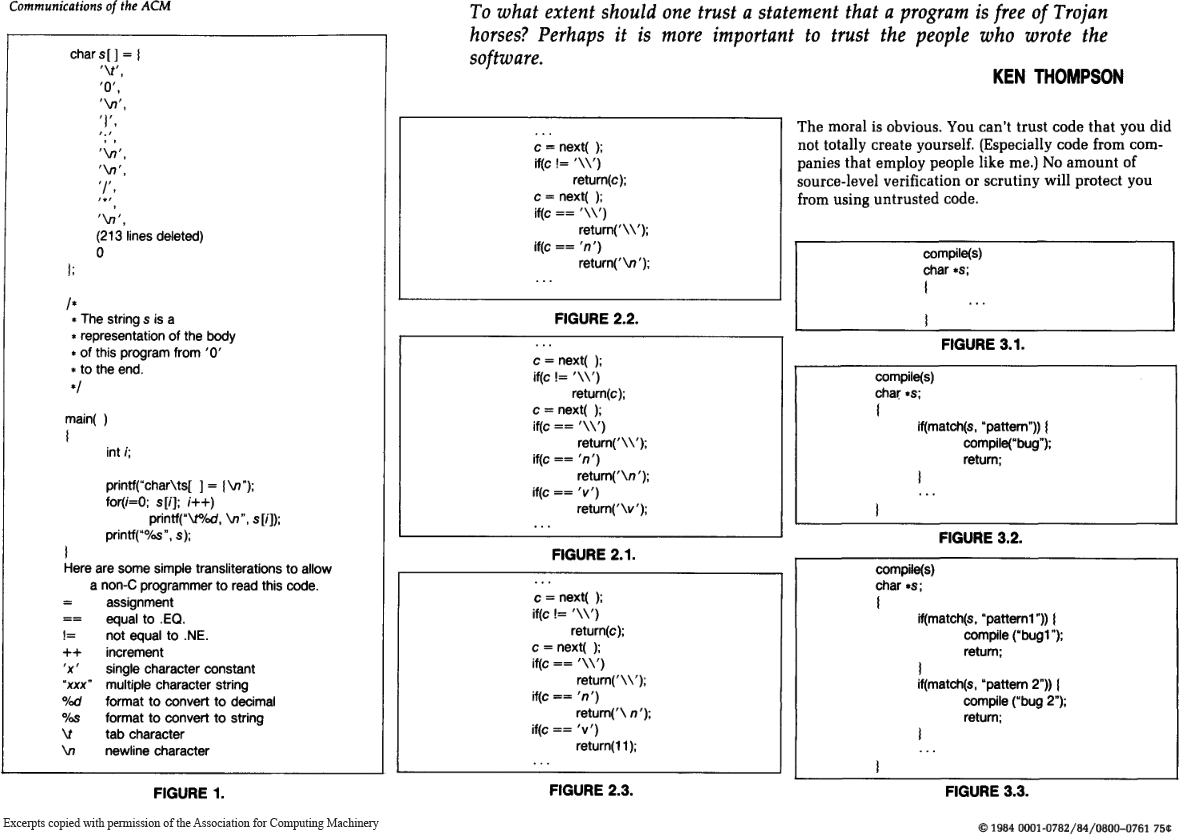
\includegraphics{assets/images/ken-thompson-hack.png}
  \caption{Excerpts from Ken Thompson's paper `Reflections on Trusting Trust'}
  \label{fig:ken-thompson-hack}
\end{figure}

Thompson demonstrated that even if you have access to the source code,
your compiler --- or any other program-handling program or
hardware --- could be compromised and detecting this backdoor would be
very difficult. Thus, in practice, a truly \textit{trustless} system does not
exist. You would have to create all your software \textit{and} all your
hardware (assemblers, compilers, linkers, etc.) from scratch, without
the aid of any external software or software-aided machinery.

\begin{quotation}
\enquote{If you wish to make an apple pie from scratch, you must first invent
the universe.}
\flushright -- Carl Sagan\footnote{Carl Sagan, \textit{Cosmos} \cite{cosmos}}
\end{quotation}

The Ken Thompson Hack is a particularly ingenious and hard-to-detect backdoor,
so let's take a quick look at a hard-to-detect backdoor which works without
modifying any software. Researchers found a way to compromise security-critical
hardware by altering the polarity of silicon
impurities.~\cite{becker2013stealthy} Just by changing the physical properties
of the stuff that computer chips are made of they were able to compromise a
cryptographically secure random number generator. Since this change can't be
seen, the backdoor can't be detected by optical inspection, which is one of the
most important tamper-detection mechanism for chips like these.

\begin{figure}
  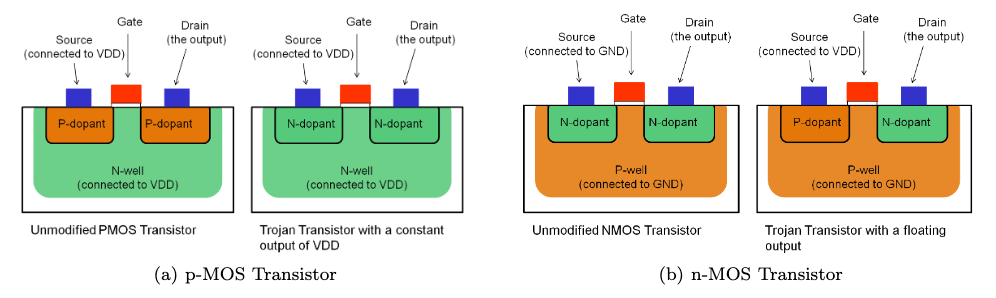
\includegraphics{assets/images/stealthy-hardware-trojan.png}
  \caption{Stealthy Dopant-Level Hardware Trojans by Becker, Regazzoni, Paar, Burleson}
  \label{fig:stealthy-hardware-trojan}
\end{figure}

Sounds scary? Well, even if you would be able to build everything from
scratch, you would still have to trust the underlying mathematics. You
would have to trust that \textit{secp256k1} is an elliptic curve without
backdoors. Yes, malicious backdoors can be inserted in the mathematical
foundations of cryptographic functions and arguably this has already
happened at least once.~\cite{wiki:Dual_EC_DRBG} There are good reasons to be paranoid, and the
fact that everything from your hardware, to your software, to the
elliptic curves used can have backdoors~\cite{wiki:backdoors} are some of them.

\begin{quotation}
``Don't trust. Verify.''
\flushright -- Bitcoiners everywhere
\end{quotation}

The above examples should illustrate that \textit{trustless} computing is
utopic. Bitcoin is probably the one system which comes closest to this
utopia, but still, it is \textit{trust-minimized} --- aiming to remove trust
wherever possible. Arguably, the chain-of-trust is neverending, since
you will also have to trust that computation requires energy, that P
does not equal NP, and that you are actually in base reality and not
emprisoned in a simulation by malicious actors.

Developers are working on tools and procedures to minimize any remaining trust
even further. For example, Bitcoin developers created
Gitian\footnote{\url{https://gitian.org/}}, which is a software distribution
method to create deterministic builds. The idea is that if multiple developers
are able to reproduce identical binaries, the chance of malicious tampering is
reduced. Fancy backdoors aren't the only attack vector. Simple blackmail or
extortion are real threats as well. As in the main protocol, decentralization is
used to minimize trust.

Various efforts are being made to improve upon the chicken-and-egg problem of
bootstrapping which Ken Thompson's hack so brilliantly pointed
out~\cite{web:bootstrapping}. One such effort is
Guix\footnote{\url{https://guix.gnu.org}} (pronounced \textit{geeks}), which
uses functionally declared package management leading to bit-for-bit
reproducible builds by design. The result is that you don't have to trust any
software-providing servers anymore since you can verify that the served binary
was not tampered with by rebuilding it from scratch. Recently, a
pull-request was merged to integrate Guix into the Bitcoin build process.\footnote{See PR 15277 of \texttt{bitcoin-core}: \\ \url{https://github.com/bitcoin/bitcoin/pull/15277}}

\begin{figure}
  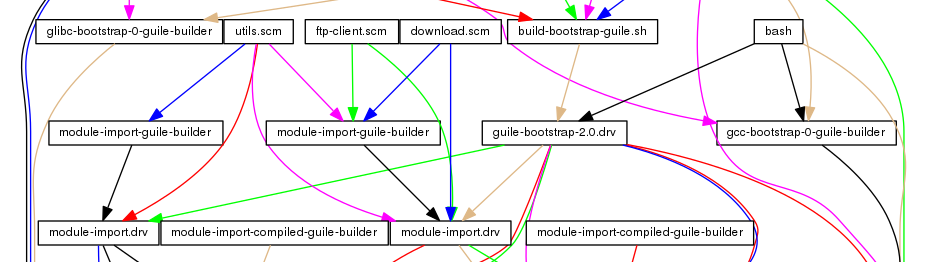
\includegraphics{assets/images/guix-bootstrap-dependencies.png}
  \caption{Which came first, the chicken or the egg?}
  \label{fig:guix-bootstrap-dependencies}
\end{figure}

Luckily, Bitcoin doesn't rely on a single algorithm or piece of
hardware. One effect of Bitcoin's radical decentralization is a
distributed security model. Although the backdoors described above are
not to be taken lightly, it is unlikely that every software wallet,
every hardware wallet, every cryptographic library, every node
implementation, and every compiler of every language is compromised.
Possible, but highly unlikely.

Note that you can generate a private key without relying on any computational
hardware or software. You can flip a coin~\cite{antonopoulos2014mastering} a
couple of times, although depending on your coin and tossing style this source
of randomness might not be sufficiently random. There is a reason why storage
protocols like Glacier\footnote{\url{https://glacierprotocol.org/}} advise to
use casino-grade dice as one of two sources of entropy.

Bitcoin forced me to reflect on what trusting nobody actually entails.
It raised my awareness of the bootstrapping problem, and the implicit
chain-of-trust in developing and running software. It also raised my
awareness of the many ways in which software and hardware can be
compromised.

\paragraph{Bitcoin taught me not to trust, but to verify.}

% ---
%
% #### Down the Rabbit Hole
%
% - [The Bitcoin whitepaper][Nakamoto] by Satoshi Nakamoto
% - [Reflections on Trusting Trust][\textit{Reflections on Trusting Trust}] by Ken Thompson
% - [51% Attack][majority] on the Bitcoin Developer Guide
% - [Bootstrapping][bootstrapping], Guix Manual
% - [Secp256k1][secp256k1] on the Bitcoin Wiki
% - [ECC Backdoors][backdoors], [Dual EC DRBG][has already happened] on Wikipedia
%
% [Emmanuel Boutet]: https://commons.wikimedia.org/wiki/User:Emmanuel.boutet
% [\textit{Reflections on Trusting Trust}]: https://www.archive.ece.cmu.edu/~ganger/712.fall02/papers/p761-thompson.pdf
% [found a way]: https://scholar.google.com/scholar?hl=en&as_sdt=0%2C5&q=Stealthy+Dopant-Level+Hardware+Trojans&btnG=
% [Gitian]: https://gitian.org/
% [bootstrapping]: https://www.gnu.org/software/guix/manual/en/html_node/Bootstrapping.html
% [Guix]: https://www.gnu.org/software/guix/
% [pull-request]: https://github.com/bitcoin/bitcoin/pull/15277
% [flip a coin]: https://github.com/bitcoinbook/bitcoinbook/blob/develop/ch04.asciidoc#private-keys
% [Glacier]: https://glacierprotocol.org/
% [secp256k1]: https://en.bitcoin.it/wiki/Secp256k1
% [majority]: https://bitcoin.org/en/developer-guide#term-51-attack
%
% <!-- Wikipedia -->
% [backdoors]: https://en.wikipedia.org/wiki/Elliptic-curve_cryptography#Backdoors
% [has already happened]: https://en.wikipedia.org/wiki/Dual_EC_DRBG
% [Carl Sagan]: https://en.wikipedia.org/wiki/Cosmos_%28Carl_Sagan_book%29
% [alice]: https://en.wikipedia.org/wiki/Alice%27s_Adventures_in_Wonderland
% [carroll]: https://en.wikipedia.org/wiki/Lewis_Carroll

\chapter{ Telling Time Takes Work}
\label{les:17}

\begin{chapquote}{Lewis Carroll, \textit{Alice in Wonderland}}
``Dear, dear! I shall be too late!''
\end{chapquote}

It is often said that bitcoins are mined because thousands of computers
work on solving *very complex* mathematical problems. Certain problems
are to be solved, and if you compute the right answer, you "produce" a
bitcoin. While this simplified view of bitcoin mining might be easier to
convey, it does miss the point somewhat. Bitcoins aren't produced or
created, and the whole ordeal is not really about solving particular
math problems. Also, the math isn't particularly complex. What is
complex is *telling the time* in a decentralized system.

As outlined in the whitepaper, the proof-of-work system (aka mining) is
a way to implement a distributed timestamp server.

\begin{figure}
  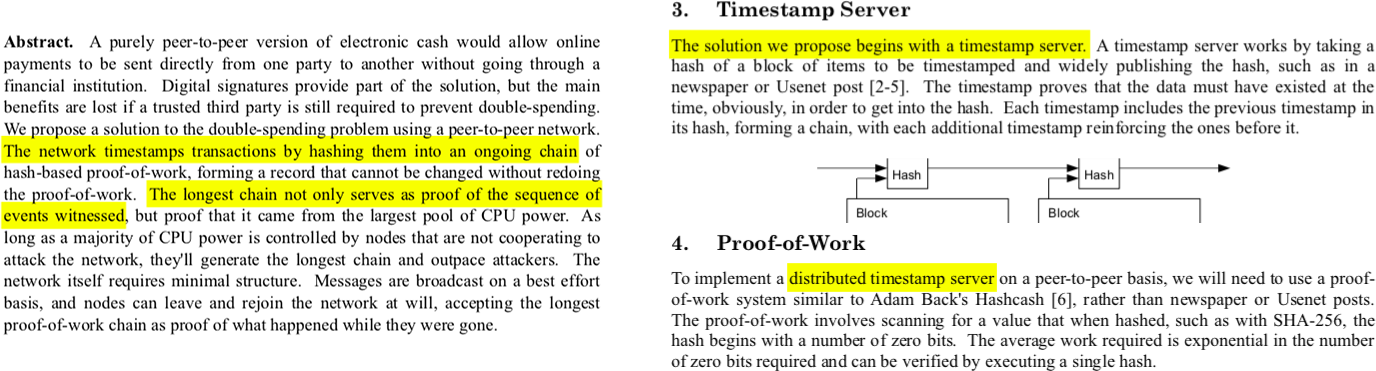
\includegraphics{assets/images/bitcoin-whitepaper-timestamp-wide.png}
  \caption{Excerpts from the whitepaper. Did someone say timechain?}
  \label{fig:bitcoin-whitepaper-timestamp-wide}
\end{figure}

When I first learned how Bitcoin works I also thought that proof-of-work
is inefficient and wasteful. After a while, I started to [shift my
perspective on Bitcoin's energy consumption][energy]. It seems that
proof-of-work is still widely misunderstood today, in the year 10 AB
(after Bitcoin).

Since the problems to be solved in proof-of-work are made up, many
people seem to believe that it is *useless* work. If the focus is purely
on the computation, this is an understandable conclusion. But Bitcoin
isn't about computation. It is about *independently agreeing on the
order of things.*

Proof-of-work is a system in which everyone can validate what happened
and in what order it happened. This independent validation is what leads
to consensus, an individual agreement by multiple parties about who owns
what.

In a radically decentralized environment, we don't have the luxury of
absolute time. Any clock would introduce a trusted third party, a
central point in the system which had to be relied upon and could be
attacked. "Timing is the root problem," as Grisha Trubetskoy [points
out]. And Satoshi brilliantly solved this problem by implementing a
decentralized clock via a proof-of-work blockchain. Everyone agrees
beforehand that the chain with the most cumulative work is the source of
truth. It is per definition what actually happened. This agreement is
what is now known as Nakamoto consensus.

\begin{quotation}
``The network timestamps transactions by hashing them into an ongoing
chain which serves as proof of the sequence of events witnessed''
\end{quotation}
% > <cite>[Satoshi Nakamoto][whitepaper]</cite>

Without a consistent way to tell the time, there is no consistent way to
tell before from after. Reliable ordering is impossible. As mentioned
above, Nakamoto consensus is Bitcoin's way to consistently tell the
time. The system's incentive structure produces a probabilistic,
decentralized clock, by utilizing both greed and self-interest of
competing participants. The fact that this clock is imprecise is
irrelevant because the order of events is eventually unambiguous and can
be verified by anyone.

Thanks to proof-of-work, both the work *and* the validation of the work
are radically decentralized. Everyone can join and leave at will, and
everyone can validate everything at all times. Not only that, but
everyone can validate the state of the system *individually*, without
having to rely on anyone else for validation.

Understanding proof-of-work takes time. It is often counter-intuitive,
and while the rules are simple, they lead to quite complex phenomena.
For me, shifting my perspective on mining helped. Useful, not useless.
Validation, not computation. Time, not blocks.

\paragraph{Bitcoin taught me that telling the time is tricky, especially if you are
decentralized.}

% ---
%
% #### Through the Looking-Glass
%
% - [Bitcoin's Energy Consumption: A shift in perspective][energy]
%
% #### Down the Rabbit Hole
%
% - [The Bitcoin whitepaper][whitepaper] by Satoshi Nakamoto
% - [Blockchain Proof-of-Work Is a Decentralized Clock][points out] by Gregory Trubetskoy
% - [The Anatomy of Proof-of-Work][pow-anatomy] by Hugo Nguyen
% - [PoW is efficient][pow-efficient] by Dan Held
% - [Mining][bw-mining], [Controlled supply][bw-supply] on the Bitcoin Wiki
%
% [points out]: https://grisha.org/blog/2018/01/23/explaining-proof-of-work/
% [energy]: 
% [whitepaper]: https://bitcoin.org/bitcoin.pdf
%
% [pow-efficient]: https://blog.picks.co/pow-is-efficient-aa3d442754d3
% [pow-anatomy]: https://bitcointechtalk.com/the-anatomy-of-proof-of-work-98c85b6f6667
% [bw-mining]: https://en.bitcoin.it/wiki/Mining
% [bw-supply]: https://en.bitcoin.it/wiki/Controlled_supply
%
% <!-- Wikipedia -->
% [alice]: https://en.wikipedia.org/wiki/Alice%27s_Adventures_in_Wonderland
% [carroll]: https://en.wikipedia.org/wiki/Lewis_Carroll

---
layout: lesson
title: Lesson 18
subtitle: Move slowly and don't break things
quote: "So the boat wound slowly along, beneath the bright summer-day, with its merry crew and its music of voices and laughter..."
categories: [bitcoin, lesson]
audio: /assets/audio/21lessons/3-18.m4a 
---

It might be a dead mantra, but "move fast and break things" is still how
much of the tech world operates. The idea that it doesn't matter if you
get things right the first time is a basic pillar of the *fail early,
fail often* mentality. Success is measured in growth, so as long as you
are growing everything is fine. If something doesn't work at first you
simply pivot and iterate. In other words: throw enough shit against the
wall and see what sticks.

Bitcoin is very different. It is different by design. It is different
out of necessity. As Satoshi [pointed out], e-currency has been tried
many times before, and all previous attempts have failed because there
was a head which could be cut off. The novelty of Bitcoin is that it is
a beast without heads.

> "A lot of people automatically dismiss e-currency as a lost cause
> because of all the companies that failed since the 1990's. I hope it's
> obvious it was only the centrally controlled nature of those systems
> that doomed them."
> <cite>[Satoshi Nakamoto][pointed out]</cite>

One consequence of this radical decentralization is an inherent
resistance to change. "Move fast and break things" does not and will
never work on the Bitcoin base layer. Even if it would be desirable, it
wouldn't be possible without convincing *everyone* to change their ways.
That's distributed consensus. That's the nature of Bitcoin.

> "The nature of Bitcoin is such that once version 0.1 was released, the
> core design was set in stone for the rest of its lifetime."
> <cite>[Satoshi Nakamoto][4]</cite>

This is one of the many paradoxical properties of Bitcoin. We all came
to believe that anything which is software can be changed easily. But
the nature of the beast makes changing it bloody hard.

As Hasu beautifully shows in [Unpacking Bitcoin's Social Contract],
changing the rules of Bitcoin is only possible by *proposing* a change,
and consequently *convincing* all users of Bitcoin to adopt this change.
This makes Bitcoin very resilient to change, even though it is software.

This resilience is one of the most important properties of Bitcoin.
Critical software systems have to be antifragile, which is what the
interplay of Bitcoin's social layer and its technical layer guarantees.
Monetary systems are adversarial by nature, and as we have known for
thousands of years solid foundations are essential in an adversarial
environment.

> "The rain came down, the floods came, and the winds blew, and beat on
> that house; and it didn't fall, for it was founded on the rock."
> <cite>[Matthew 7:24--27]</cite>

Arguably, in this parable of the wise and the foolish builders Bitcoin
isn't the house. It is the rock. Unchangeable, unmoving, providing the
foundation for a new financial system.

Just like geologists, who know that rock formations are always moving
and evolving, one can see that Bitcoin is always moving and evolving as
well. You just have to know where to look and how to look at it.

The introduction of [pay to script hash] and [segregated witness] are
proof that Bitcoin's rules can be changed if enough users are convinced
that adopting said change is to the benefit of the network. The latter
enabled the development of the [lightning network], which is one of the
houses being built on Bitcoin's solid foundation. Future upgrades like
[Schnorr signatures] will enhance efficiency and privacy, as well as
scripts (read: smart contracts) which will be indistinguishable from
regular transactions thanks to [Taproot]. Wise builders do indeed build
on solid foundations.

Satoshi wasn't only a wise builder technologically. He also understood
that it would be necessary to make wise decisions ideologically.

> "Being open source means anyone can independently review the code. If
> it was closed source, nobody could verify the security. I think it's
> essential for a program of this nature to be open source."
> <cite>[Satoshi Nakamoto][5]</cite>

Openness is paramount to security and inherent in open source and the
free software movement. As Satoshi pointed out, secure protocols and the
code which implements them have to be open --- there is no security
through obscurity. Another benefit is again related to decentralization:
code which can be run, studied, modified, copied, and distributed freely
ensures that it is spread far and wide.

The radically decentralized nature of Bitcoin is what makes it move
slowly and deliberately. A network of nodes, each run by a sovereign
individual, is inherently resistant to change --- malicious or not. With
no way to force updates upon users the only way to introduce changes is
by slowly convincing each and every one of those individuals to adopt a
change. This non-central process of introducing and deploying changes is
what makes the network incredibly resilient to malicious changes. It is
also what makes fixing broken things more difficult than in a
centralized environment, which is why everyone tries not to break things
in the first place.

Bitcoin taught me that moving slowly is one of its features, not a bug.

---

#### Through the Looking-Glass

- [Lesson 1: Immutability and Change][lesson1]

#### Down the Rabbit Hole

- [Unpacking Bitcoin's Social Contract] by Hasu
- [Schnorr signatures BIP][Schnorr signatures] by Pieter Wuille
- [Taproot proposal][Taproot] by Gregory Maxwell
- [P2SH][pay to script hash], [SegWit][segregated witness] on the Bitcoin Wiki
- [Parable of the Wise and the Foolish Builders][Matthew 7:24--27] on Wikipedia

<!-- Down the Rabbit Hole -->
[lesson1]: {{ '/bitcoin/lessons/ch1-01-immutability-and-change' | absolute_url }}

[pointed out]: http://p2pfoundation.ning.com/forum/topics/bitcoin-open-source?commentId=2003008%3AComment%3A9493
[4]: https://bitcointalk.org/index.php?topic=195.msg1611#msg1611
[Unpacking Bitcoin's Social Contract]: https://uncommoncore.co/unpacking-bitcoins-social-contract/
[Matthew 7:24--27]: https://en.wikipedia.org/wiki/Parable_of_the_Wise_and_the_Foolish_Builders
[pay to script hash]: https://en.bitcoin.it/wiki/Pay_to_script_hash
[segregated witness]: https://en.bitcoin.it/wiki/Segregated_Witness
[lightning network]: https://lightning.network/
[Schnorr signatures]: https://github.com/sipa/bips/blob/bip-schnorr/bip-schnorr.mediawiki#cite_ref-6-0
[Taproot]: https://lists.linuxfoundation.org/pipermail/bitcoin-dev/2018-January/015614.html
[5]: https://bitcointalk.org/index.php?topic=13.msg46#msg46

<!-- Wikipedia -->
[alice]: https://en.wikipedia.org/wiki/Alice%27s_Adventures_in_Wonderland
[carroll]: https://en.wikipedia.org/wiki/Lewis_Carroll

\chapter{Lesson 19: Privacy is not Dead}
\label{les:19}

\blockquote{
The players all played at once without waiting for turns, and quarrelled all
the while at the tops of their voices, and in a very few minutes the Queen was
in a furious passion, and went stamping about and shouting ``off with his
head!'' of ``off with her head!'' about once in a minute.
}

If pundits are to believed, privacy has been dead [since the 80ies]. The
pseudonymous invention of Bitcoin and other events in recent history
show that this is not the case. Privacy is alive, even though it is by
no means easy to escape the surveillance state.

Satoshi went through great lengths to cover up his tracks and conceal
his identity. Ten years later, it is still unknown if Satoshi Nakamoto
was a single person, a group of people, male, female, or a
[time-traveling AI] which bootstrapped itself to take over the world.
Conspiracy theories aside, Satoshi chose to identify himself to be a
Japanese male, which is why I don't assume but respect his chosen gender
and refer to him as *he*.

% 

Whatever his real identity might be, Satoshi was successful in hiding
it. He set an encouraging example for everyone who wishes to remain
anonymous: it is possible to have privacy online.

\begin{quotation}
``Encryption works. Properly implemented strong crypto systems are one
of the few things that you can rely on.''
\end{quotation}
% > <cite>[Edward Snowden]</cite>

Satoshi wasn't the first pseudonymous or anonymous inventor, and he
won't be the last. Some have directly imitated this pseudonymous
publication style, like Tom Elvis Yedusor of [MimbleWimble] fame, while
others have published advanced mathematical proofs while remaining
completely [anonymous].

It is a strange new world we are living in. A world where identity is
optional, contributions are accepted based on merit, and people can
collaborate and transact freely. It will take some adjustment to get
comfortable with these new paradigms, but I strongly believe that all of
this has the potential to change the world for the better.

We should all remember that privacy is a [fundamental human right]. And
as long as people exercise and defend these rights the battle for
privacy is far from over. Bitcoin taught me that privacy is not dead.

% ---
%
% #### Down the Rabbit Hole
%
% - [Universal Declaration of Human Rights][fundamental human right] by the United Nations
% - [A lower bound on the length of the shortest superpattern][anonymous] by Anonymous 4chan Poster, Robin Houston, Jay Pantone, and Vince Vatter
%
% [since the 80ies]: https://books.google.com/ngrams/graph?content=privacy+is+dead&year_start=1970&year_end=2019&corpus=15&smoothing=3&share=&direct_url=t1%3B%2Cprivacy%20is%20dead%3B%2Cc0
% [time-traveling AI]: https://blockchain24-7.com/is-crypto-creator-a-time-travelling-ai/
% ["I am not Dorian Nakamoto."]: http://p2pfoundation.ning.com/forum/topics/bitcoin-open-source?commentId=2003008%3AComment%3A52186
% [Edward Snowden]: https://www.theguardian.com/world/2013/jun/17/edward-snowden-nsa-files-whistleblower
% [MimbleWimble]: https://github.com/mimblewimble/docs/wiki/MimbleWimble-Origin
% [anonymous]: https://oeis.org/A180632/a180632.pdf
% [fundamental human right]: http://www.un.org/en/universal-declaration-human-rights/
%
% <!-- Wikipedia -->
% [alice]: https://en.wikipedia.org/wiki/Alice%27s_Adventures_in_Wonderland
% [carroll]: https://en.wikipedia.org/wiki/Lewis_Carroll

\chapter{Lesson 20: Cypherpunks Write Code}
\label{les:20}

\blockquote{
``I see you're trying to invent something.''
}

Like many great ideas, Bitcoin didn't come out of nowhere. It was made
possible by utilizing and combining many innovations and discoveries in
mathematics, physics, computer science, and other fields. While
undoubtedly a genius, Satoshi wouldn't have been able to invent Bitcoin
without the giants on whose shoulders he was standing on.

\begin{quotation}
``He who only wishes and hopes does not interfere actively with the
course of events and with the shaping of his own destiny.''
\end{quotation}
% > <cite>[Ludwig Von Mises]</cite>

One of these giants is Eric Hughes, one of the founders of the
cypherpunk movement and author of the [cypherpunk manifesto]. It's hard
to imagine that Satoshi wasn't influenced by this manifesto. It speaks
of many things which Bitcoin enables and utilizes, such as direct and
private transactions, electronic money and cash, anonymous systems, and
defending privacy with cryptography and digital signatures.

\begin{quotation}
``Privacy is necessary for an open society in the electronic age.
[...] Since we desire privacy, we must ensure that each party to a
transaction have knowledge only of that which is directly necessary
for that transaction. [...]
Therefore, privacy in an open society requires anonymous transaction
systems. Until now, cash has been the primary such system. An
anonymous transaction system is not a secret transaction system.
[...]
We the Cypherpunks are dedicated to building anonymous systems. We are
defending our privacy with cryptography, with anonymous mail
forwarding systems, with digital signatures, and with electronic
money.
Cypherpunks write code.''
\end{quotation}
% > <cite>[Eric Hughes][cypherpunk manifesto]</cite>

Cypherpunks do not find comfort in hopes and wishes. They actively
interfere with the course of events and shape their own destiny.
Cypherpunks write code.

Thus, in true cypherpunk fashion, Satoshi sat down and started to write
code. Code which took an abstract idea and proved to the world that it
actually worked. Code which planted the seed of a new economic reality.
Thanks to this code, everyone can verify that this novel system actually
works, and every 10 minutes or so Bitcoin proofs to the world that it is
still living.

% 

To make sure that his innovation transcends fantasy and becomes reality,
Satoshi wrote code to implement his idea before he wrote the whitepaper.
He also made sure [not to delay] any release forever. After all,
"there's always going to be one more thing to do."

\begin{quotation}
``I had to write all the code before I could convince myself that I
could solve every problem, then I wrote the paper.''
\end{quotation}
% > <cite>[Satoshi Nakamoto][6]</cite>

In today's world of endless promises and doubtful execution, an exercise
in dedicated building was desperately needed. Be deliberate, convince
yourself that you can actually solve the problems, and implement the
solutions. We should all aim to be a bit more cypherpunk.

Bitcoin taught me that cypherpunks write code.

% ---
%
% #### Down the Rabbit Hole
%
% - [A Cypherpunk's Manifesto][cypherpunk manifesto] by Eric Hughes
% - [Bitcoin version 0.1.0 announcement][version 0.1.0] by Satoshi Nakamoto
% - [Bitcoin P2P e-cash paper announcement][mail-announcement] by Satoshi Nakamoto
%
% [mail-announcement]: http://www.metzdowd.com/pipermail/cryptography/2008-October/014810.html
% [Ludwig Von Mises]: https://mises.org/library/human-action-0/html/pp/613
% [cypherpunk manifesto]: https://www.activism.net/cypherpunk/manifesto.html
% [version 0.1.0]: https://bitcointalk.org/index.php?topic=68121.0
% [not to delay]: https://bitcointalk.org/index.php?topic=199.msg1670#msg1670
% [6]: http://www.metzdowd.com/pipermail/cryptography/2008-November/014832.html
%
% <!-- Wikipedia -->
% [alice]: https://en.wikipedia.org/wiki/Alice%27s_Adventures_in_Wonderland
% [carroll]: https://en.wikipedia.org/wiki/Lewis_Carroll

\chapter{Metaphors for Bitcoin's Future}
\label{les:21}

\begin{chapquote}{Lewis Carroll, \textit{Alice in Wonderland}}
\enquote{I know something interesting is sure to happen\ldots}
\end{chapquote}

In the last couple of decades, it became apparent that technological
innovation does not follow a linear trend. Whether you believe in the
technological singularity or not, it is undeniable that progress is
exponential in many fields. Not only that, but the rate at which
technologies are being adopted is accelerating, and before you know it
the bush in the local schoolyard is gone and your kids are using
Snapchat instead. Exponential curves have the tendency to slap you in
the face way before you see them coming.

Bitcoin is an exponential technology built upon exponential technologies.
\textit{Our World in Data}\footnote{\url{https://ourworldindata.org/}}
beautifully shows the rising speed of technological adoption, starting in 1903
with the introduction of landlines. Landlines, electricity, computers, the
internet, smartphones; all follow exponential trends in price-performance and
adoption. Bitcoin does too~\cite{tech-adoption}.

\begin{figure}
  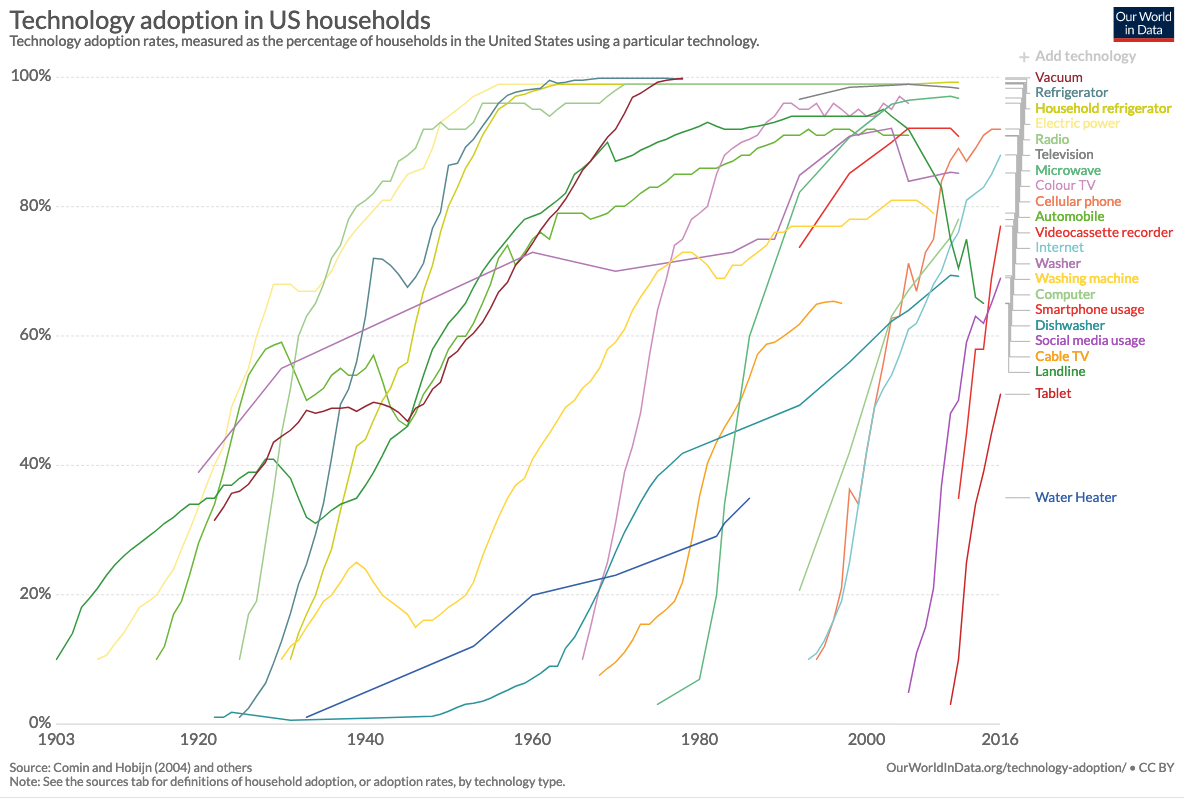
\includegraphics{assets/images/tech-adoption.png}
  \caption{Bitcoin is literally off the charts.}
  \label{fig:tech-adoption}
\end{figure}

Bitcoin has not one but multiple network effects\footnote{Trace Mayer,
\textit{The Seven Network Effects of Bitcoin}~\cite{7-network-effects}}, all of
which resulting in exponential growth patterns in their respective area: price,
users, security, developers, market share, and adoption as global money.

Having survived its infancy, Bitcoin is continuing to grow every day in
more aspects than one. Granted, the technology has not reached maturity
yet. It might be in its adolescence. But if the technology is
exponential, the path from obscurity to ubiquity is short.

\begin{figure}
  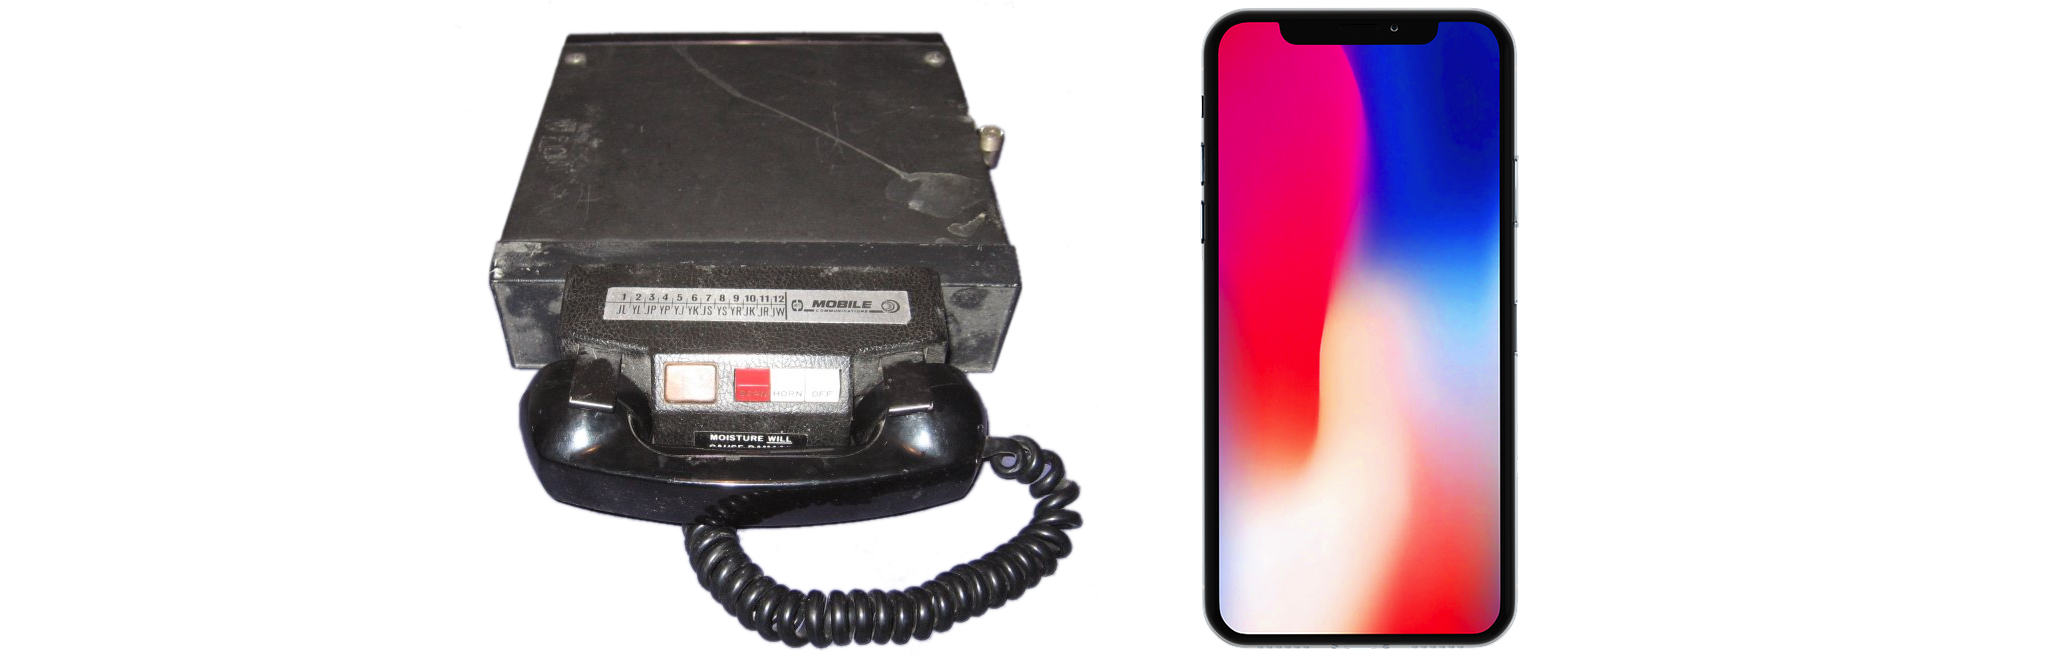
\includegraphics{assets/images/mobile-phone.png}
  \caption{Mobile phone, ca 1965 vs 2019.}
  \label{fig:mobile-phone}
\end{figure}

In his 2003 TED talk, Jeff Bezos chose to use electricity as a metaphor for the
web's future.\footnote{\url{http://bit.ly/bezos-web}} All three phenomena ---
electricity, the internet, Bitcoin --- are \textit{enabling} technologies,
networks which enable other things. They are infrastructure to be built upon,
foundational in nature.

Electricity has been around for a while now. We take it for granted. The
internet is quite a bit younger, but most people already take it for
granted as well. Bitcoin is ten years old and has entered public
consciousness during the last hype cycle. Only the earliest of adopters
take it for granted. As more time passes, more and more people will
recognize Bitcoin as something which simply is.\footnote{This is known as the
\textit{Lindy Effect}. The Lindy effect is a theory that the future life expectancy
of some non-perishable things like a technology or an idea is proportional to
their current age, so that every additional period of survival implies a longer
remaining life expectancy.~\cite{wiki:lindy}}

In 1994, the internet was still confusing and unintuitive. Watching this old
recording of the \textit{Today
Show}\footnote{\url{https://youtu.be/UlJku_CSyNg}} makes it obvious that what
feels natural and intuitive now actually wasn't back then. Bitcoin is still
confusing and alien to most, but just like the internet is second nature for
digital natives, spending and stacking
sats\footnote{\url{https://twitter.com/hashtag/stackingsats}} will be second
nature to the bitcoin natives of the future.

\begin{quotation}\begin{samepage}
\enquote{The future is already here --- it's just not very evenly
distributed.}
\begin{flushright} -- William Gibson\footnote{William Gibson, \textit{The Science in Science Fiction} \cite{william-gibson}}
\end{flushright}\end{samepage}\end{quotation}

In 1995, about $15\%$ of American adults used the internet. Historical
data from the Pew Research Center~\cite{pew-research} shows how the internet has woven
itself into all our lives. According to a consumer survey by Kaspersky
Lab~\cite{web:kaspersky}, 13\% of respondents have used Bitcoin and its clones to pay for
goods in 2018. While payments aren't the only use-case of bitcoin, it is
some indication of where we are in Internet time: in the early- to
mid-90s.

In 1997, Jeff Bezos stated in a letter to shareholders~\cite{bezos-letter} that
\enquote{this is Day 1 for the Internet,} recognizing the great untapped
potential for the internet and, by extension, his company. Whatever day this is
for Bitcoin, the vast amounts of untapped potential are clear to all but the
most casual observer.

\begin{figure}
  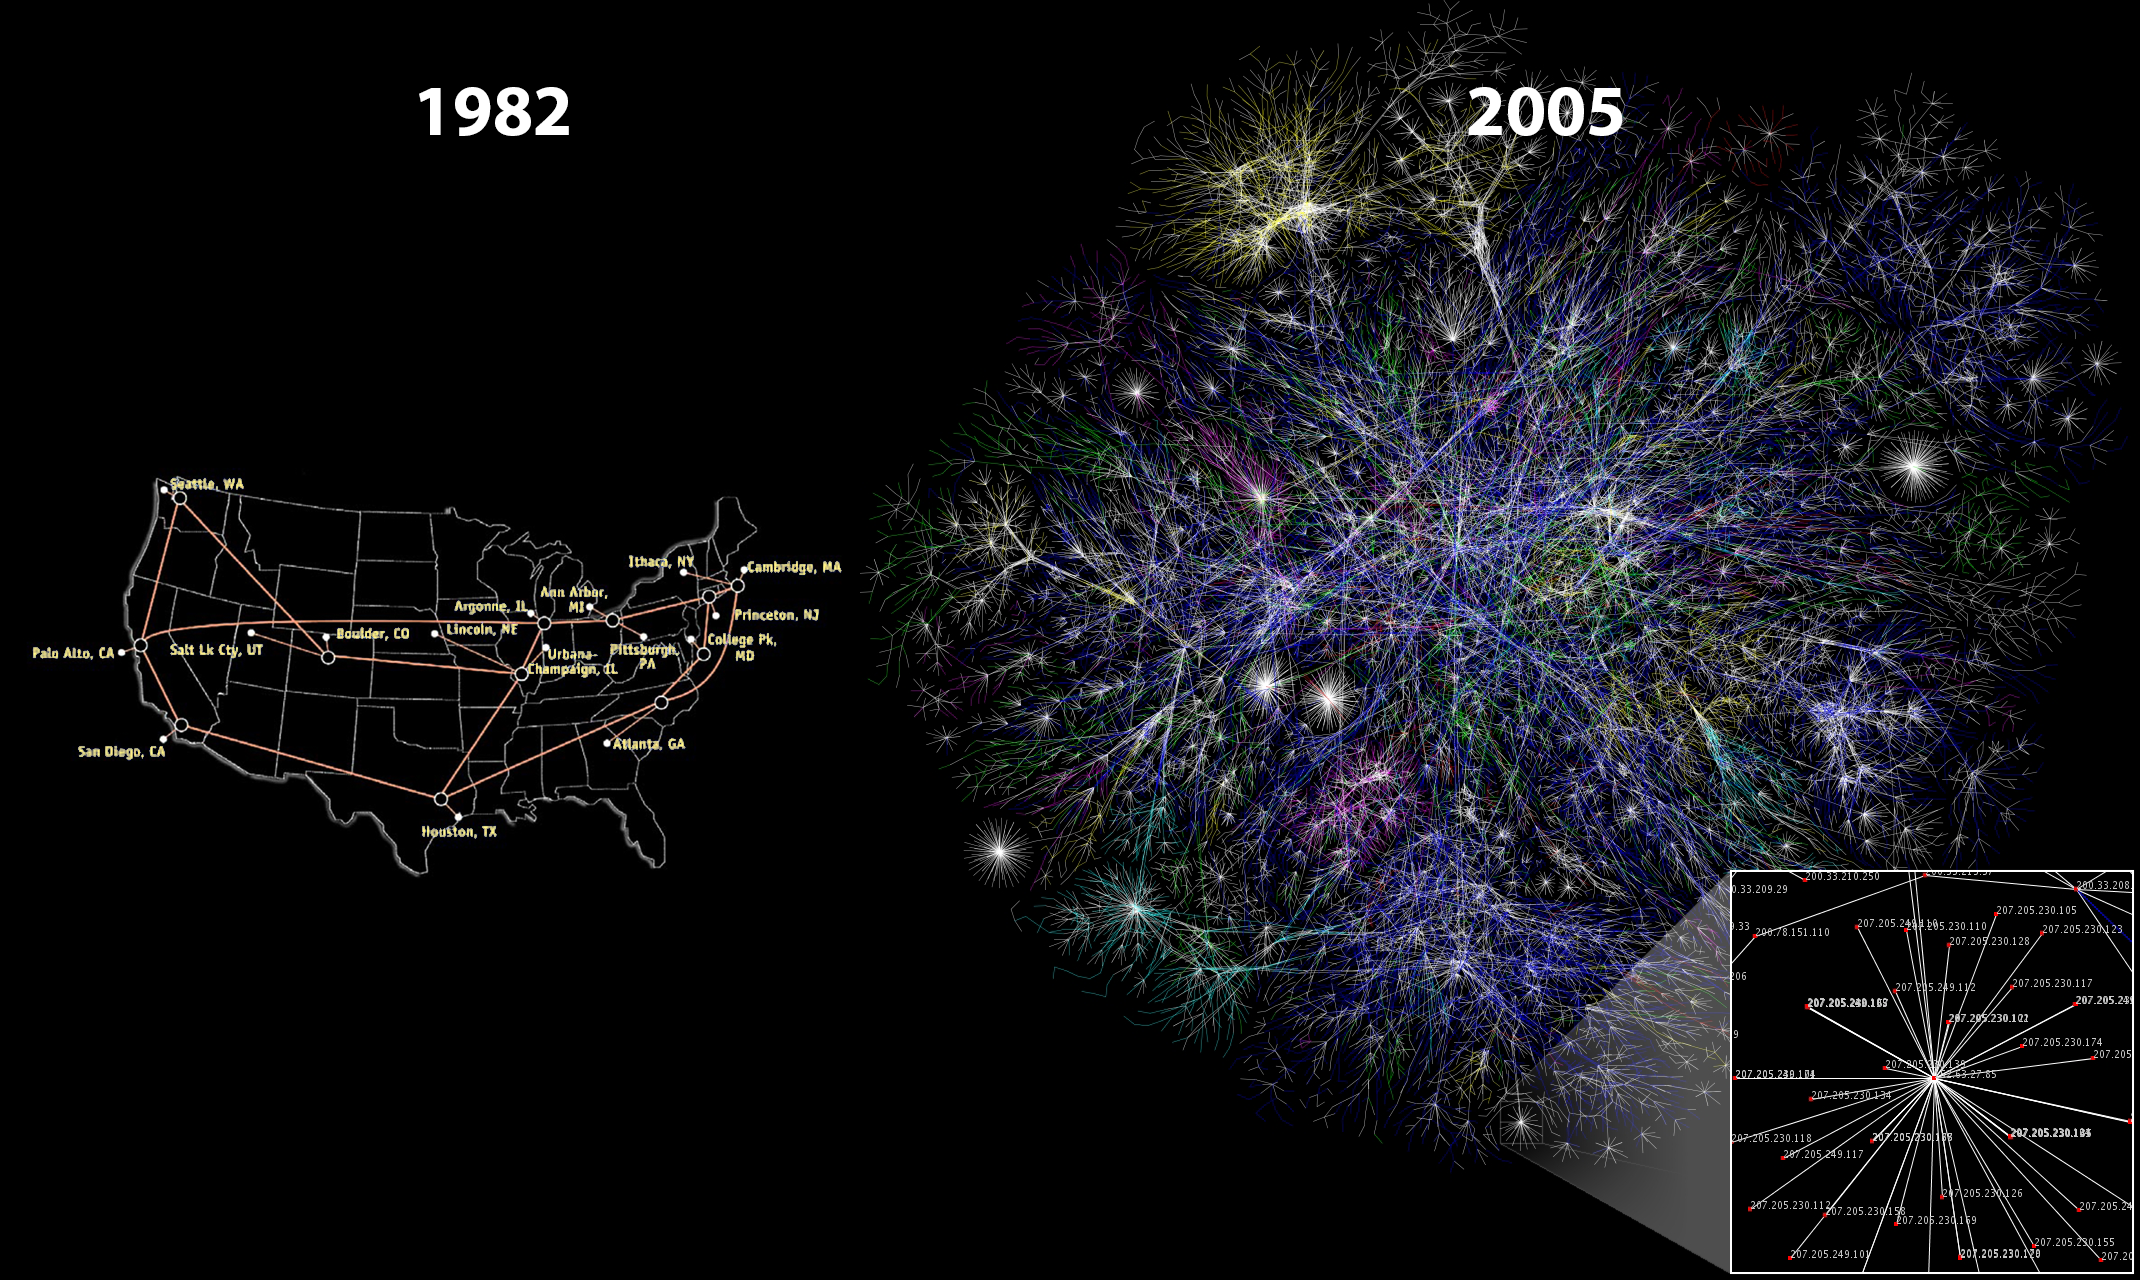
\includegraphics{assets/images/internet-evolution-black-dates.png}
  \caption{The internet, 1982 vs 2005. Source: cc-by Merit Network, Inc. and Barrett Lyon, Opte Project}
  \label{fig:internet-evolution-black-dates}
\end{figure}

Bitcoin's first node went online in 2009 after Satoshi mined the \textit{genesis
block}\footnote{The genesis block is the first block of the Bitcoin block chain.
Modern versions of Bitcoin number it as block $0$, though very early versions
counted it as block $1$. The genesis block is usually hardcoded into the
software of the applications that utilize the Bitcoin block chain. It is a
special case in that it does not reference a previous block and produces an
unspendable subsidy. The \textit{coinbase} parameter contains, along with the
normal data, the following text: \textit{\enquote{The Times 03/Jan/2009 Chancellor on
brink of second bailout for banks}} \cite{btcwiki:genesis-block}} and released
the software into the wild. His node wasn't alone for long. Hal Finney was one
of the first people to pick up on the idea and join the network. Ten years
later, as of this writing, more than
$75.000$\footnote{\url{https://bit.ly/luke-nodecount}} nodes are running
bitcoin.

\begin{figure}
  \centering
  
\includegraphics[width=8cm]{assets/images/running-bitcoin.png}
  \caption{Hal Finney authored the first tweet mentioning bitcoin in January 2009.}
  \label{fig:running-bitcoin}
\end{figure}

The protocol's base layer isn't the only thing growing exponentially.
The lightning network, a second layer technology, is growing at an even
faster rate.

In January 2018, the lightning network had $40$ nodes and $60$
channels~\cite{web:lightning-nodes}. In April 2019, the network grew to more
than $4000$ nodes and around $40.000$ channels. Keep in mind that this is still
experimental technology where loss of funds can and does occur. Yet the trend is
clear: thousands of people are reckless and eager to use it.

\begin{figure}
  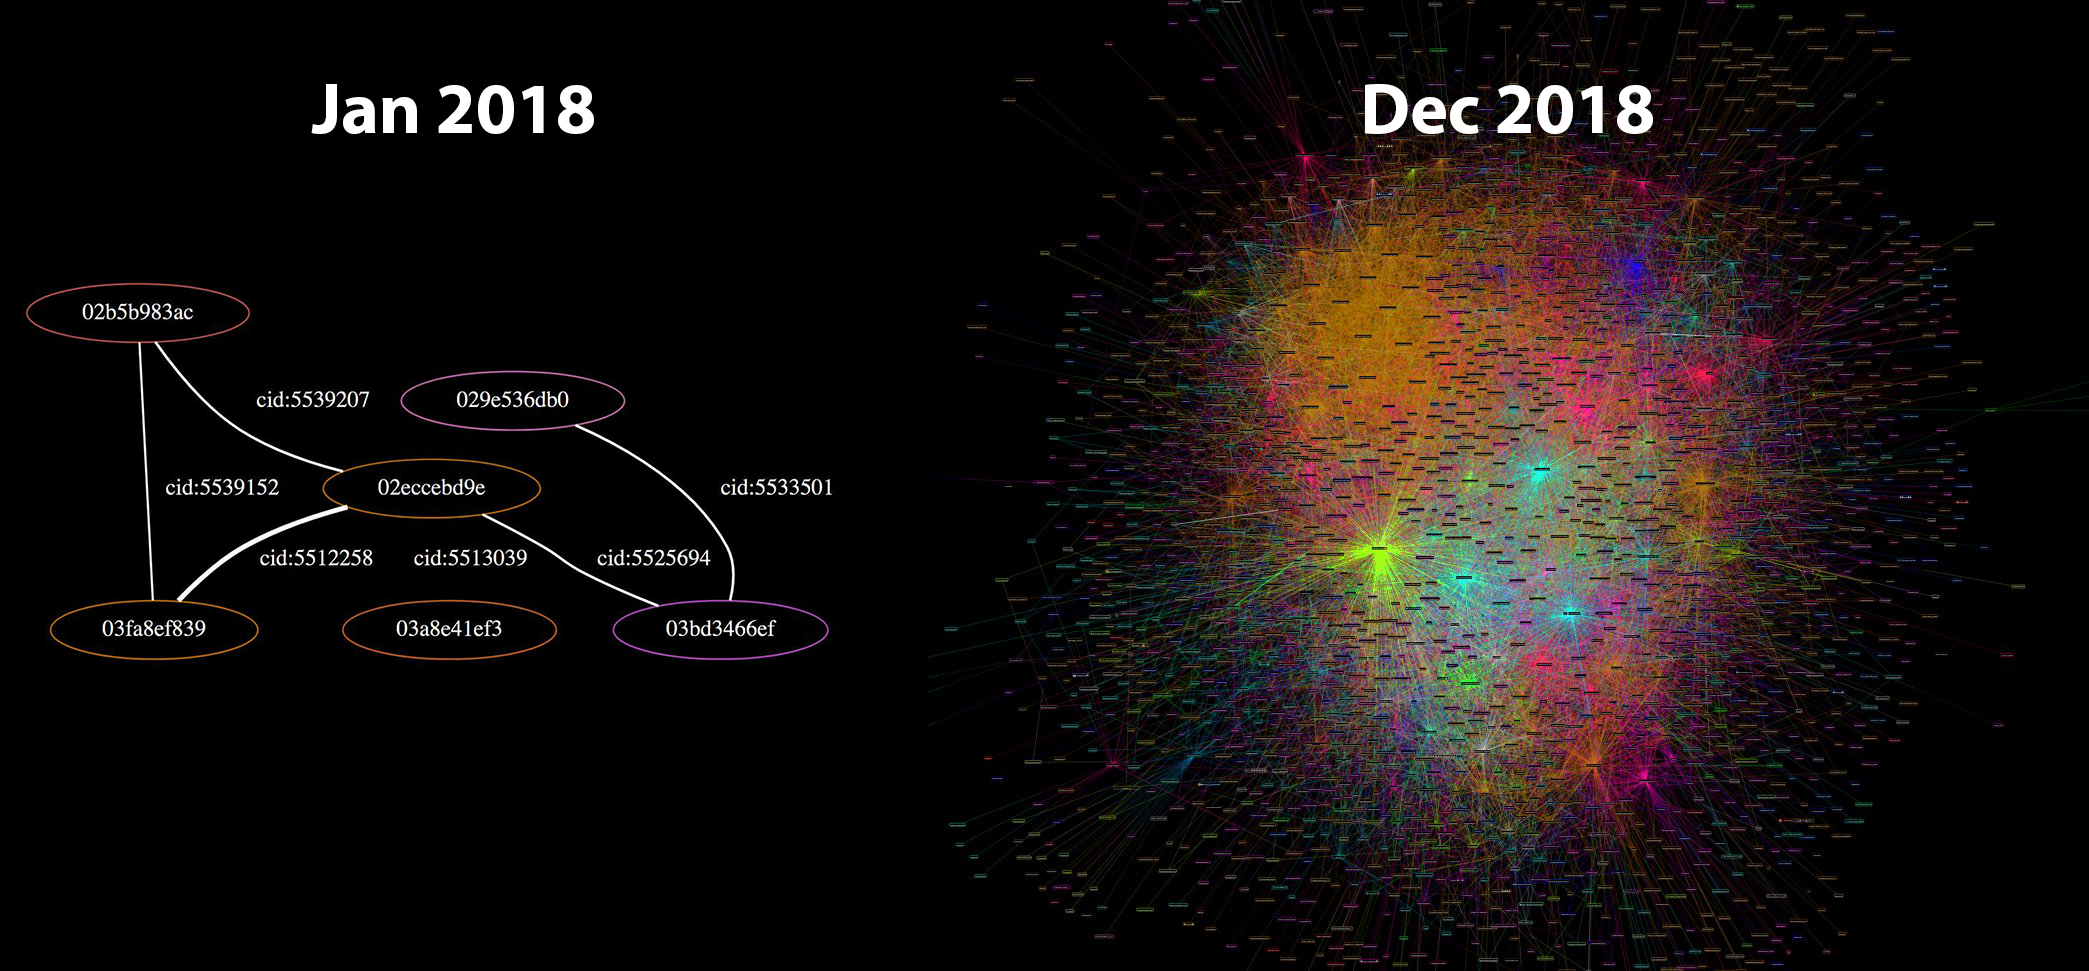
\includegraphics{assets/images/lnd-growth-lopp-black.png}
  \caption{Lightning Network, January 2018 vs December 2018. Source: Jameson Lopp}
  \label{fig:lnd-growth-lopp-black.png}
\end{figure}

To me, having lived through the meteoric rise of the web, the parallels
between the internet and Bitcoin are obvious. Both are networks, both
are exponential technologies, and both enable new possibilities, new
industries, new ways of life. Just like electricity was the best
metaphor to understand where the internet is heading, the internet might
be the best metaphor to understand where bitcoin is heading. Or, in the
words of Andreas Antonopoulos, Bitcoin is \textit{The Internet of Money}.
These metaphors are a great reminder that while history doesn't repeat
itself, it often rhymes.

Exponential technologies are hard to grasp and often underestimated.
Even though I have a great interest in such technologies, I am
constantly surprised by the pace of progress and innovation. Watching
the Bitcoin ecosystem grow is like watching the rise of the internet in
fast-forward. It is exhilarating.

My quest of trying to make sense of Bitcoin has led me down the pathways
of history in more ways than one. Understanding ancient societal
structures, past monies, and how communication networks evolved were all
part of the journey. From the handaxe to the smartphone, technology has
undoubtedly changed our world many times over. Networked technologies
are especially transformational: writing, roads, electricity, the
internet. All of them changed the world. Bitcoin has changed mine and
will continue to change the minds and hearts of those who dare to use
it.

\paragraph{Bitcoin taught me that understanding the past is essential to
understanding its future. A future which is just beginning\ldots}

% ---
%
% #### Down the Rabbit Hole
%
% - [The Rising Speed of Technological Adoption][the rising speed of technological adoption] by Jeff Desjardins
% - [The 7 Network Effects of Bitcoin][multiple network effects] by Trace Mayer
% - [The Electricity Metaphor for the Web's Future][TED talk] by Jeff Bezos
% - [How the internet has woven itself into American life][data from the Pew Research Center] by Susannah Fox and Lee Rainie
% - [Genesis Block][genesis block] on the Bitcoin Wiki
% - [Lindy Effect][more time] on Wikipedia
%
% [Our World in Data]: https://ourworldindata.org/
% [the rising speed of technological adoption]: https://www.visualcapitalist.com/rising-speed-technological-adoption/
% [multiple network effects]: https://www.thrivenotes.com/the-7-network-effects-of-bitcoin/
% [TED talk]: https://www.ted.com/talks/jeff_bezos_on_the_next_web_innovation
% [recording of the Today Show]: https://www.youtube.com/watch?v=UlJku_CSyNg
% [William Gibson]: https://www.npr.org/2018/10/22/1067220/the-science-in-science-fiction
% [data from the Pew Research Center]: https://www.pewinternet.org/2014/02/27/part-1-how-the-internet-has-woven-itself-into-american-life/
% [consumer survey]: https://www.kaspersky.com/blog/money-report-2018/
% [letter to shareholders]: http://media.corporate-ir.net/media_files/irol/97/97664/reports/Shareholderletter97.pdf
% [running bitcoin]: https://twitter.com/halfin/status/1110302988?lang=en
% [40 nodes]: https://bitcoinist.com/bitcoin-lightning-network-mainnet-nodes/
% [reckless]: https://twitter.com/hashtag/reckless
% [Jameson Lopp]: https://twitter.com/lopp/status/1077200836072296449
% [\textit{The Internet of Money}]: https://theinternetofmoney.info/
% [stacking]: https://twitter.com/hashtag/stackingsats
%
% <!-- Bitcoin Wiki -->
% [genesis block]: https://en.bitcoin.it/wiki/Genesis_block
%
% <!-- Wikipedia -->
% [more time]: https://en.wikipedia.org/wiki/Lindy_effect
% [alice]: https://en.wikipedia.org/wiki/Alice%27s_Adventures_in_Wonderland
% [carroll]: https://en.wikipedia.org/wiki/Lewis_Carroll

\addpart{Conclusion}
\label{ch:conclusion}

\begin{chapquote}{Lewis Carroll, \textit{Alice in Wonderland}}
``Begin at the beginning'' the King said, very gravely, ``and go on till you
come to the end: then stop.''
\end{chapquote}

\textit{As mentioned in the beginning}, I think that any answer to the
question *“What have you learned from Bitcoin?”* will always be incomplete. The
symbiosis of what can be seen as multiple living systems -- Bitcoin, the
technosphere, and economics -- is too intertwined, the topics too numerous, and
things are moving too fast to ever be fully understood by a single person.

Even without understanding it fully, and even with all its quirks and seeming
shortcomings, Bitcoin undoubtedly works. It keeps producing blocks roughly every
ten minutes and does so beautifully. The longer Bitcoin continues to work, the
more people will opt-in to use it.

\begin{quotation}
``It's true that things are beautiful when they work. Art is function.'' \flushright
-- Giannina Braschi
\end{quotation}

\textit{Bitcoin is a child of the internet}. It is growing exponentially,
blurring the lines between disciplines. It isn’t clear, for example, where the
realm of pure technology ends and where another realm begins. Even though
Bitcoin requires computers to function efficiently, computer science is not
sufficient to understand it. Bitcoin is not only borderless in regards to its
inner workings but also boundaryless in respect to academic disciplines.

Economics, politics, game theory, monetary history, network theory, finance,
cryptography, information theory, censorship, law and regulation, human
organization, psychology -- all these and more are areas of expertise which might
help in the quest of understanding how Bitcoin works and what Bitcoin is.

No single invention is responsible for its success. It is the combination of
multiple, previously unrelated pieces, glued together by game theoretical
incentives, which make up the revolution that is Bitcoin. The beautiful blend of
many disciplines is what makes Satoshi a genius.

\textit{Like every complex system}, Bitcoin has to make tradeoffs in terms
of efficiency, cost, security, and many other properties. Just like there is no
perfect solution to deriving a square from a circle, any solution to the
problems which Bitcoin tries to solve will always be imperfect as well.

% > “I don’t believe we shall ever have a good money again before we take the
% > thing out of the hands of government, that is, we can’t take it violently
% > out of the hands of government, all we can do is by some sly roundabout way
% > introduce something that they can’t stop.”
% > <cite>[Friedrich Hayek][sly roundabout way]</cite>

Bitcoin is the sly, roundabout way to re-introduce good money to the world. It
does so by placing a sovereign individual behind each node, just like Da Vinci
tried to solve the intractable problem of squaring a circle by placing the
Vitruvian Man in its center. Nodes effectively remove any concept of a center,
creating a system which is astonishingly antifragile and extremely hard to shut
down. Bitcoin lives, and its heartbeat will probably outlast all of ours.

I hope you have enjoyed these twenty-one lessons. Maybe the most important
lesson is that Bitcoin should be examined holistically, from multiple angles, if
one would like to have something approximating a complete picture. Just like
removing one part from a complex system destroys the whole, examining parts of
Bitcoin in isolation seems to taint the understanding of it. If only one person
strikes "blockchain" from her vocabulary and replaces it with "a chain of
blocks" I will die a happy man.

In any case, my journey continues. I plan to venture further down into the
depths of this rabbit hole, and I invite you to [tag along][dergigi] for the ride.

% <!-- Twitter -->
% [dergigi]: https://twitter.com/dergigi
%
% <!-- Internal -->
% [sly roundabout way]: https://youtu.be/EYhEDxFwFRU?t=1124
% [Giannina Braschi]: https://en.wikipedia.org/wiki/Braschi%27s_Empire_of_Dreams


\listoffigures

\bibliography{main}

\end{document}
